\documentclass[12pt,twoside]{report}
%General
\newcommand{\breakhere}{\noindent\rule{15cm}{0.4pt}}
\newcommand{\qm}{\textbf{\textcolor{red}{?}}}
\newcommand*\plus{\ensuremath{\texttt{+}}~}
\newcommand*\plusn{\ensuremath{\texttt{+}}}
\newcommand*\hy{\ensuremath{\mbox{-}}}

% Chapter 4
\providecommand{\httwo}{\ensuremath{H_{\mathrm{T,2}}/2}\xspace}
\providecommand{\ptone}{\ensuremath{p_{\mathrm{T,1}}}\xspace}
\providecommand{\pttwo}{\ensuremath{p_{\mathrm{T,2}}}\xspace}
\providecommand{\cme}{$\sqrt{s}$\xspace}
\providecommand{\MadGraphF}{{\textsc{MadGraph5}}\xspace}






% Itemize
\newcommand*\ball{\setbeamertemplate{itemize items}[ball]}
\newcommand*\cir{\setbeamertemplate{itemize items}[circle]}
\newcommand*\tri{\setbeamertemplate{itemize items}[triangle]}

%Colors
%\newcommand*\mycolor{\textcolor{red!80!black}}
%\newcommand*\blue{\textcolor{blue!70!black}}
%\newcommand*\green{\textcolor{green!50!black}}
%\definecolor{auburn}{rgb}{0.07, 0.04, 0.56}
\newcommand*\AN{\textcolor{auburn}}
\newcommand*\yes{\textcolor{red!80!black} {\Checkmark }}
\newcommand*\no{\textcolor{red!80!black} {\XSolidBrush}}
%\definecolor{pink}{rgb}{1.0, 0.11, 0.81}
%spaces
\newcommand{\tab}[1]{\hspace{.2\textwidth}\rlap{#1}}
\newcommand{\itab}[1]{\hspace{.12\textwidth}\rlap{#1}}
%\tcbset{colframe=white,colback=white,nobeforeafter}
\newcommand{\mybox}[2]{{\color{red!80!black}\fbox{\normalcolor#2}}}
\setlength\fboxrule{0.8pt}
%Def
\newcommand{\lumins}{\ensuremath{\mathcal{L}}}

\providecommand{\ptave}{\ensuremath{\langle p_\mathrm{T1,2}\rangle}\xspace}
\providecommand{\bqm}{\ensuremath{\scalebox{1.2}{\textbf{?}}}\xspace}
\providecommand{\RooUnfold} {{\textsc{RooUnfold}}\xspace}
\providecommand{\refe}{\ensuremath{\textcolor{red!80!black}{\bf [REF]}}\xspace}
\providecommand{\HERWIGPP} {{\textsc{herwig++}}\xspace}
\providecommand{\PYTHIAS} {{\textsc{pythia6}}\xspace}
\providecommand{\PYTHIAE} {{\textsc{pythia8}}\xspace}
\providecommand{\POWHEG} {{\textsc{powheg}}\xspace}
\providecommand{\NLOJETPP} {{\textsc{NLOJet++}}\xspace}
\providecommand{\RunDec}{{\textsc{RunDec}}\xspace}
\providecommand{\fastNLO} {{\textsc{fastNLO}}\xspace}
\providecommand{\fastjet} {{\textsc{FastJet}}\xspace}
\providecommand{\mur}{\ensuremath{\mu_r}\xspace}
\providecommand{\muf}{\ensuremath{\mu_f}\xspace}
\providecommand{\alpsmz}{\ensuremath{\alpha_s(M_Z)}\xspace}
\providecommand{\chisq}{\ensuremath{\chi^2}\xspace}
\providecommand{\chisqndof}{\ensuremath{\chi^2/n_\mathrm{dof}}\xspace}
\providecommand{\alps}{\ensuremath{\alpha_S}\xspace}
\providecommand{\alpsmusq}{\ensuremath{\alpha_S(\mu_r^2)}\xspace}
\providecommand{\alpsmzsq}{\ensuremath{\alpha_S(M_Z^2)}\xspace}
\providecommand{\alpsqsq}{\ensuremath{\alpha_S(Q^2)}\xspace}
\providecommand{\alpsmu}{\ensuremath{\alpha_S(\mu_r)}\xspace}
\providecommand{\alpsmz}{\ensuremath{\alpha_S(M_Z)}\xspace}
\providecommand{\alpsq}{\ensuremath{\alpha_S(Q)}\xspace}
\providecommand{\ratio}{\ensuremath{R_{32}}\xspace}
\providecommand{\LHAPDF}{{\textsc{LHAPDF}}\xspace}
\providecommand{\LHAPDFS}{{\textsc{LHAPDF6}}\xspace}
\providecommand{\NF}{\ensuremath{N_F}\xspace}
\providecommand{\Ztwostar}{\ensuremath{\mathrm{Z2}^\star}\xspace}
\newcommand{\hftwo}{\hspace*{\fill}}
\newcommand{\rbthm}{\rule[-2ex]{0ex}{5ex}}
\newcommand{\rbtrr}{\rule[-0.8ex]{0ex}{3.2ex}}
\newcommand*\alpsmzns{\ensuremath{\alpha_S(M_Z)}}
\newcommand*\alpsns{\ensuremath{\alpha_S}}
\newcommand*\httwons{\ensuremath{\mathrm{H_{T,2}}/2}}
\newcommand*\ptavens{\ensuremath{\mathrm{\langle p_\mathrm{T_{1,2}}\rangle}}}
\newcommand*\rations{\ensuremath{\mathrm{R_{32}}}}

\newcommand*\pas{\includegraphics[scale=0.3]{/home/anter/Desktop/Analysis_8/Present_Latex/Pre-approval/Plots/pas_new.png}}
\newcommand*\staru{\ensuremath{\blue{^{*}}}}
\newcommand*\unc{\ensuremath{\blue{^{\#}}}}
\newcommand*\pts{p$^2_{\mathrm{T}}$}
\newcommand*\msd{m$_{\mathrm{SD}}$}
\newcommand*\msds{m$^2_{\mathrm{SD}}$}
\newcommand*\met{E$\mathrm{_{T}^{miss}}$}
\newcommand*\varnd{$\mathrm{N_{2,DDT}^1}$}
\newcommand*\vartau{$\mathrm{\tau_{21}^{DDT}}$}
\newcommand*\varn{$\mathrm{N_{2}^1}$}
\newcommand*\rapa{$\mathrm{|\eta|}$}
\newcommand*\gr{$\mathrm{>}~$}
\newcommand*\ls{$\mathrm{<}~$}
\newcommand{\inv}{$^{\text{-}1}$}



\usepackage{array}
\usepackage{commath}
\usepackage{fancyhdr}
\usepackage{graphicx,psfrag,amsmath}
\usepackage{nccmath}
\usepackage{lineno}
\usepackage{multibib}
\usepackage{url}
\usepackage{multirow}     
\usepackage[usenames,dvipsnames]{color}
\usepackage{setspace}
\usepackage[margin=16pt,font={small,stretch=1.1}]{caption}
\usepackage[usenames,dvipsnames]{color}
\usepackage[caption=false]{subfig}
\usepackage{cite}
\usepackage{rotating}
\usepackage{pdfpages}
\usepackage{gensymb}
\usepackage{bold-extra}
\usepackage[italic]{hepnames}
\usepackage{ptdr-definitions}
\usepackage[english]{babel}
\usepackage[utf8]{inputenc}
\usepackage[belowskip=-1pt,aboveskip=2pt]{caption}

\setlength{\headheight}{15pt} 
\usepackage[pdfpagelabels]{hyperref}
%%%\renewcommand{\familydefault}{\sfdefault}
%\hypersetup{colorlinks,
%  citecolor=Red,
%  linkcolor=blue,
%  urlcolor=magenta}
\pagestyle{fancy} \fancyhfoffset[LE]{.5 cm}
\clearpage{\pagestyle{empty}\cleardoublepage} \pagestyle{fancy}

\renewcommand{\chaptermark}[1]{\markboth{\chaptername\ \thechapter}{}}
\renewcommand{\sectionmark}[1]{\markright{\thesection\ #1}}
\fancyhf{}

\fancyhead[LE,RO]{\thepage} \fancyhead[LO]{\slshape\rightmark}
\fancyhead[RE]{\slshape\leftmark}

\textheight 23 cm \textwidth 15cm
\oddsidemargin 1.05 cm \evensidemargin -0.2 cm
\topmargin -0.8 cm \tolerance=10000000

\newtheorem{theorem}{Theorem}
\setlength{\parindent}{1 cm}
\setlength{\parskip}{0.14 cm}
\linespread{1.5}
\raggedbottom

\def\st{\scriptstyle}
\def\sst{\scriptscriptstyle}
\def\mco{\multicolumn}
\def\fr{\frac}
\def\no{\nonumber}
\def\pd{\partial}
\def\be{\begin{equation}}
\def\ee{\end{equation}}
\def\bea{\begin{eqnarray}}
\def\eea{\end{eqnarray}}
\def\sech{{\rm{sech}}}
\def\r{\ref}

\setcounter{page}{1} \setcounter{secnumdepth}{3}
\setcounter{tocdepth}{3}

\usepackage{bookmark}

\begin{document}

{
\pagestyle{empty}
\begin{center}
\renewcommand{\rmdefault}{phv} % Arial
%\renewcommand{\sfdefault}{phv} % Arial
{\fontsize{14}{16}\sf \bf MEASUREMENT OF MULTIJET CROSS-SECTION RATIOS IN PROTON-PROTON COLLISIONS WITH THE CMS DETECTOR AT THE LHC}
\\ [3.8cm]

{\fontsize{12}{14} \sf A THESIS} \\
\vspace{0.3cm}
{ \sf Submitted to the \\
{\fontsize{12}{14} FACULTY OF SCIENCE \\
PANJAB UNIVERSITY, CHANDIGARH \\ }
for the degree of }\\
\vspace{0.5cm}
{\fontsize{14}{16}  \bf DOCTOR OF PHILOSOPHY}\\ [2.0cm]
{\fontsize{14}{16} \sf \textbf{2017}} \\[2.0cm]
{\fontsize{14}{16} \bf Anterpreet Kaur}\\[1.25cm]
{\fontsize{12}{14} \sf DEPARTMENT OF PHYSICS \\
CENTRE OF ADVANCED STUDY IN PHYSICS\\
PANJAB UNIVERSITY, CHANDIGARH\\
INDIA}
\end{center}

}

\newpage 
\thispagestyle{empty}

\pagenumbering{roman}
%% --- dedication page ---

\baselineskip=1pc \lineskip=1pc \lineskiplimit=1pc
\renewcommand{\thepage}{\roman{page}}
\setcounter{page}{2}
%
\mbox{}\newpage

\vspace*{2in}
\begin{center}
{\bf\emph{\Large
Dedicated to\\
my Grand-Parents\\
~~~~~\&\\
~~~Parents\\
}}
\end{center}
\vskip 4pc

\newpage\thispagestyle{empty}
\mbox{}\newpage

\hypersetup{pageanchor=false}
\cleardoublepage
%\phantomsection
%\addcontentsline{toc}{chapter}{Acknowledgements}
%\include{MyAck}

\newpage\thispagestyle{empty}
\mbox{}\newpage

\cleardoublepage
%\phantomsection
%\addcontentsline{toc}{chapter}{Abstract}
%\include{abstract_one}

\newpage\thispagestyle{empty}
\mbox{}\newpage

\tableofcontents
\newpage\thispagestyle{empty}
\mbox{}\newpage

\cleardoublepage
\phantomsection
\addcontentsline{toc}{chapter}{List of Figures}
\begin{spacing}{1.15}
\listoffigures
\end{spacing}

\cleardoublepage
\phantomsection
\addcontentsline{toc}{chapter}{List of Tables}
\addtocontents{toc}{\protect\rule{13.9 cm}{.1pt}\par}
\listoftables
\newpage

\pagenumbering{arabic}

%%\chapter{Introduction}
\label{chap:Introduction}

Particle physics deals with the study of the basic constituents of matter and the forces governing the interactions among them. The Standard Model (SM) is the most accepted theory describing the nature and properties of the fundamental particles and their interactions. The elementary particles leptons and quarks, known as fermions, interact through the exchange of the gauge bosons. The gauge bosons acquire masses in the process of electroweak symmetry breaking whereas the masses of the fermions are generated through Yukawa interactions with the field associated to the scalar Higgs boson. The gauge bosons are the mediators of the four fundamental forces of interaction existing in nature : the electromagnetic force, the strong force, the weak force and the gravitational force. Quantum Choromodynamics (QCD) is the theory of the strong interactions between the quarks mediated by the massless gluons. The quarks and gluons, together known as partons, have a peculiar property of ``color'' charge. Due to confinement property of QCD, the quarks cannot exist freely in nature but bind themselves into colorless particles called hadrons such as protons and neutrons together known as nucleons, pions etc. The structure and the properties of sub-atomic particles can be explored by first accelerating them using particle accelerators and then colliding at very high energies. The end products of these collisions are recorded in particle detectors in the form of data sets which are analyzed in detail to reveal the structure and characteristic properties of the fundamental particles.

To search for the very rare particles, to investigate the physics beyond SM, and to explore the regime of undiscovered physical laws, the particle accelerators have become bigger and more complex over the past few decades. The Large Hadron Collider (LHC) is one of the biggest and the most powerful particle collider in which protons are accelerated and collided at extremely high center-of-mass energies to probe their internal structure and the parton distribution functions (PDFs). The PDFs give the probability to find a parton at an energy scale Q carrying a fractional momentum $x$ of the proton. Since the proton is not elementary and is made up of partons, the proton-proton (pp) collisions are viewed as interactions between their constituent partons. The final products of the scattering are observed by Compact Muon Solenoid (CMS), one of the four detectors of the LHC, located at the interaction points of the collisions. The scattering cross-section can be expressed as a sum in terms of increasing powers of the strong coupling constant $\alpha_{S}$ convoluted with PDFs. The lowest-order $\alpha_{S}^{2}$ term represents the production of two partons in final states whereas terms of higher-order $\alps^3$, $\alps^4$ etc. signify the existence of multi-partons in final states. The highly energetic final state partons emit quarks and gluons with lower energies and give rise to a parton shower (PS). The colored products of PS hadronize to a spray of colorless hadrons known as jets. The jets are the final structures observed in the detector. So they carry the significant information of the energy and direction of the initial partons and hence are important to study. The final partons also have the probability to radiate more gluons and quarks which also hadronize and result in multijets in the final state. At LHC, such events are produced in large number and are an important source for testing the predictions given by QCD. They also serve as an important background in the searches for new particles and physics beyond SM. 

The inclusive multijet event cross-section $\sigma_{i\hy{\rm jet}}$, given by the process ${{\rm pp}\to i~{\rm jets}~\plus X}$, is proportional to $\alpha^{i}_{s}$. The study of inclusive jet cross-sections in terms of jet transverse momentum \pt and rapidity $y$ is very important because it provides the essential information about the PDFs and the precise measurement of \alps. Also the ratio of cross-sections given by Eq.~\ref{eq:ratio_mn} is proportional to the QCD coupling constant \alps and hence can be used to determine the value of \alps. 

\begin{equation}
R_{mn} = \frac{\sigma_{m\hy {\rm jet}}}{\sigma_{n\hy {\rm jet}}} \propto \alps^{m-n}
\label{eq:ratio_mn}
\end{equation}

Instead of studying inclusive cross-sections, the cross-section ratio is more useful because of the partial or complete cancellation of many theoretical and experimental uncertainties in the ratio. The CMS Collaboration has previously measured the ratio of the inclusive 3-jet cross-section to that of the inclusive 2-jet as a function of the average transverse momentum, $<p_{T1,2}>$, of the two leading jets in the event at 7 TeV \cite {Chatrchyan:2013txa}. This study leads to an extraction of \alpsmz = 0.1148 $\pm$ 0.0055, where the dominant uncertainty stems from the estimation of higher-order corrections to the next-to-leading order (NLO) predictions. In this thesis, a measurement of inclusive 2-jet and 3-jet event cross-sections as well as ratio of 3-jet event cross-section over 2-jet \rations, is performed using an event sample collected during 2012 by the CMS experiment at the LHC and corresponding to an integrated luminosity of 19.7\fbinv of pp collisions at a center-of-mass energy of 8\TeV. The event scale is chosen to be the average transverse momentum of the two leading jets, referred to as \httwo in this thesis. The strength of the strong force, \alps at a given energy scale $Q$ is not predicted and has to be extracted from the experiment. Hence, the value of the strong coupling constant at the scale of the $Z$ boson mass \alpsmz is extracted from the measurements performed in this thesis. The value of \alps depends on the energy scale $Q$ and it decreases with the increase of $Q$ scale. The running of \alps with scale $Q$ is also studied and compared with other CMS measurements as well as results from different experiments. This checks the consistency with QCD via the renormalization group equation (RGE)\footnote{According to the RGE, the strong force becomes weaker at short distances corresponding to large momentum transfers. This is referred to a property of QCD called asymptotic freedom.}, which precisely describes the evolution of \alps with the renormalization scale of QCD. 

The organization of this thesis\footnote{The common unit convention based on International System of Units (SI) as followed in particle physics will be used throughout the thesis. In addition, the units electron volt (eV) and barn (b) are used for energy and interaction cross-section, respectively. The reduced Planck constant ($\hbar$) and speed of light ($c$) are set to unity, i.e. $\hbar$ = c = 1. The electric charge Q is expressed in units of elementary charge $e$} is as follows :

{\bf Chapter~\ref{chap:Theory}} gives a brief overview of the Standard Model of particle physics and the theory of strong interactions QCD, theory of hadron collisions as well as formation of jets and jet algorithms. 

{\bf Chapter~\ref{chap:Detector}} deals with experimental apparatus which covers the details of the geometry of the CMS detector and its various sub-detectors.

{\bf Chapter~\ref{chap:Reconstruction}} describes the methods of event generation used in different Monte Carlo event generators, detector geometry simulation and reconstruction of the particles in the detector. This chapter also gives the details of the different approaches of jet reconstruction at CMS and applied jet-energy corrections along with the description of the software framework used in the analysis presented in the current thesis.

{\bf Chapter~\ref{chap:Measurement}} presents the measurement of differential inclusive multijet event cross-sections and the cross-section ratio. The measurements are corrected for detector effects by unfolding procedure which is discussed in detail in this chapter. The sources of the experimental uncertainties are studied in detail. 

{\bf Chapter~\ref{chap:Theory_Predictions}} contains a detailed description of the NLO perturbative QCD theory predictions obtained using different PDF sets. The NLO predictions are corrected with the non-perturbative and electroweak corrections. The theoretical uncertainties are calculated from various sources. At the end of this chapter, the unfolded measurements are compared with the predictions at NLO in pQCD as well as with the predictions from several Monte Carlo event generators.

{\bf Chapter~\ref{chap:Alphas}} describes the method to extract the strong coupling constant at the scale of mass of $Z$ boson \alpsmz from the measurements of differential inclusive multijet cross-sections and the cross-section ratio \ratio. Also, the running of \alps with energy scale Q is presented along with the previous measurements from different experiments.

{\bf Chapter~\ref{chap:Summary}} summarizes the results and conclusions of the work done in this thesis.

{\bf Chapter~\ref{chap:Hardware}} mentions the participation in other hardware and software activities.
  %Chapter 1
%%\chapter{Theoretical Background}
\label{chap:Theory}
Since 1930s, many theories and discoveries in particle physics have revealed the fundamental structure of matter. The matter is made up of fundamental particles and their interactions are mediated by four fundamental forces \cite{Griffiths:111880}. The theoretical models strive to describe all the phenomena of particle physics and properties of particles. These models must be either confirmed experimentally or totally excluded giving hints of new physics. This interplay between experimental discoveries and the corresponding theoretical predictions leads to a theoretical model called Standard Model, which describes the fundamental particles and their interactions. The world's most powerful particle accelerators and detectors are used by physicists to test the predictions and limits of the Standard Model where it has successfully explained almost all experimental results. This chapter describes the Standard Model with main focus on the theory of strong interactions called Quantum Chromodynamics and its features which serve as the theoretical base of this thesis.

%The growing knowledge about fundamental and new particles was accompanied by the evolution of quantum mechanics and the special relativity. 
\section{Standard Model}
The Standard Model (SM) of particle physics \cite{Perkins:1982xb,Herrero:1998eq,Weinberg:1967tq} was developed in 1970s. It is a mathematical framework which describes the nature and properties of the fundamental particles and the three of the four known interactions between them, as summarized in Fig.~\ref{fig:SM}. According to the SM, the basic constituents of matter are fermions and bosons. The fermions have half integral spin and obey Fermi-Dirac statistics. They follow the Pauli exclusion principle according to which two or more identical fermions cannot occupy the same quantum state. Each fermion has an associated anti-particle having the same properties but opposite-sign quantum numbers.
\begin{figure}[!h]
\begin{center}
\hspace*{-5mm}
%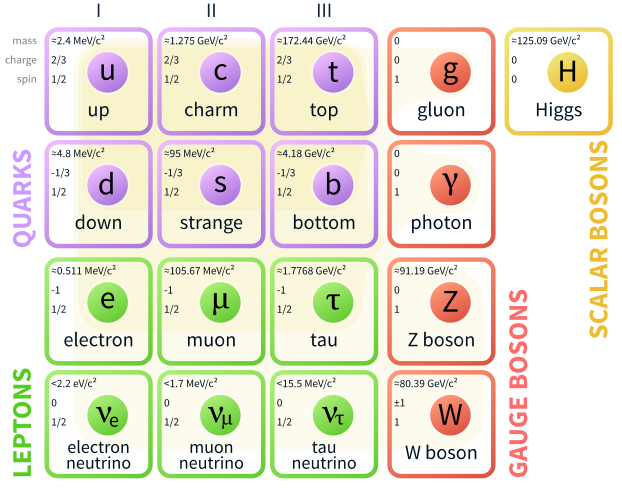
\includegraphics[scale = 0.8]{/home/anter/Desktop/Thesis/Figures/StandardModel_edited.png}\\
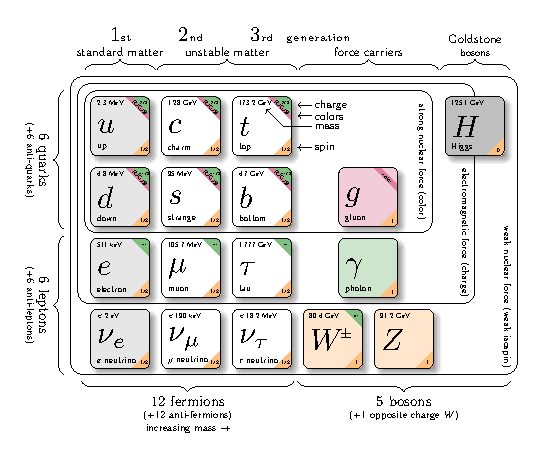
\includegraphics[width=1.0\textwidth]{/home/anter/Desktop/Thesis/Figures/model-physics.pdf}\\
%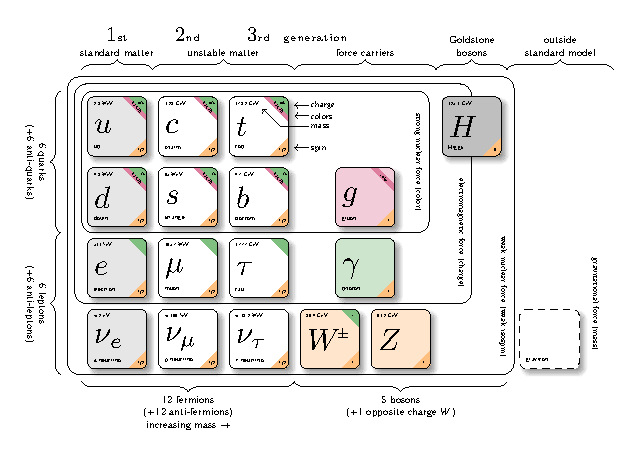
\includegraphics[width=1.2\textwidth]{/home/anter/Desktop/Thesis/Figures/original_model-physics.pdf}\\
\caption[The Standard Model summarizing the properties of elementary particles and their forces of interaction.]{The Standard Model\footnotemark summarizing the properties of elementary particles known as fermions (leptons and quarks) grouped into three generations, gauge bosons as mediators for the interactions and the scalar Higgs boson.}% and not incorporated graviton for the gravitational force.}
\label{fig:SM}
\end{center}
\end{figure}
\footnotetext{Source : \url{http://www.texample.net/tikz/examples/model-physics}}%https://en.wikipedia.org/wiki/Standard_Model}}

Depending on how the fermions interact, these are classified into two categories - leptons (\sln) and quarks ($q$). The leptons are of six types : electron ($e$), muon ($\mu$) and tau ($\tau$) with electric charge Q = -1 and the corresponding neutrinos : electron neutrino ($\nu_e$), muon neutrino ($\nu_\mu$) and tau neutrino ($\nu_\tau$) having electric charge Q = 0. The quarks exist in six ``flavors'' : up ($u$), down ($d$), strange ($s$), charm ($c$), bottom ($b$) and top ($t$). $u$, $c$ and $t$ carry electric charge Q = \plusn$\frac{2}{3}$ whereas $d$, $s$ and $b$ carry Q = -$\frac{1}{3}$. The quarks and leptons are categorized into three generations. The first generation has the lightest and the most stable particles whereas the heavier and less stable particles belong to the second and third generations.

The elementary bosons have integral spin and obey the Bose-Einstein statistics. These are further of two types : gauge bosons having non-zero integral spin and a scalar boson with zero spin. The gauge bosons are the force carriers which mediate the electromagnetic, strong, weak and gravitational forces. Every interaction involves the exchange of a gauge boson : the massless photon ($\gamma$) for the electromagnetic force, massless gluons ($g$) for the strong force, massive $W^\pm$ and $Z$ for the weak force and the graviton (not yet found) for the gravitational force. However, the gravitational force has not been incorporated into SM yet. Along with this, the existence of dark matter or dark energy and the matter-antimatter asymmetry are still missing pieces in the SM. The interaction between fundamental particles acts because of some peculiar property of the particles - charge for the electromagnetic force, color for the strong force and flavor for the weak force. 

The SM framework based on quantum field theories \cite{Peskin:1995ev} is described by SU(3)$_{\rm C}~\otimes$ SU(2)$_{\rm L}~\otimes$ U(1)$_{\rm Y}$ gauge symmetry where C stands for the color charge, L for weak isospin and Y for hypercharge\footnote{Hypercharge Y = Q - ${\rm T}_{3}$, where Q is the electric charge and and ${\rm T}_{3}$ is the third component of weak isospin.}. Here SU(3)$_{\rm C}$, SU(2)$_{\rm L}$ and U(1)$_{\rm Y}$ terms give rise to strong, weak and electromagnetic forces, respectively. U($n$) are the unitary and SU($n$) are the special unitary groups of degree $n$. The SU(3)$_{\rm C}$ term defines the strong interaction between quarks and gluons mediated by gluons, with the three degrees of freedom of the color charge (C). The electromagnetic interaction of particles is explained by the most precise theory, today known as Quantum Electrodynamics (QED). In SM, the weak and electromagnetic interactions are combined by an electroweak symmetry theory \cite{Glashow:1979pj,Salam:1980jd}, described by SU(2)$_{\rm L}~\otimes$ U(1)$_{\rm Y}$ gauge group. But this electroweak unification could not explain the occurrence of massive weak gauge bosons. This problem was solved by Higgs mechanism \cite{Higgs:1964pj,Englert:1964et}. The Higgs boson, named after Peter Higgs, is the field quantum of the Higgs field responsible for electroweak symmetry breaking. In SM, the Higgs field is a SU(2) doublet which is a scalar under Lorentz transformations. The coupling of the bosons to the scalar Higgs field causes the spontaneous symmetry breaking which triggers the Higgs mechanism. After symmetry breaking, three of the four degrees of freedom in the Higgs field interact with the three weak gauge bosons ($W^\pm$ and $Z$) and allows them to be massive, while the remaining one degree of freedom becomes the Higgs boson. Its existence was confirmed by the CMS \cite{Chatrchyan:2012xdj} and ATLAS \cite{Aad:2012tfa} collaborations in 2012, with properties consistent with the SM. In contrast to the electroweak symmetry, the SU(3)$_{\rm C}$ of the strong interaction is an exact symmetry and hence the gluons are massless. The strong interaction between quarks and gluons is described by quantum chromodynamics (QCD), explained in detail in the next section.%Georgi:1974sy

%The gauge bosons of the unified electroweak theory are a mixture of the gauge bosons of the unbroken symmetry
\section{Quantum Chromodynamics}
The strong interactions between the quarks and gluons are described by a non-abelian gauge theory called quantum chromodynamics (QCD) \cite{Ellis:1991qj, Halzen:1984mc}. The gauge group of QCD is the special unitary group SU(3)$_{\rm C}$ with color charges C as the generators of the gauge group. Color charge is the peculiar property of QCD and has a similar role as the electric charge in electromagnetic interactions. However, the mediator of electromagnetic interactions, i.e. the photon itself does not carry any electric charge whereas the gluon itself carry color charge. This allows the self coupling of gluons and hence makes the theory non-abelian. Both the quarks and gluons carry three types of color charges : red ($r$), green ($g$) and blue ($b$), and three types of anti-color charges : anti-red ($\bar{r}$), anti-green ($\bar{g}$) and anti-blue ($\bar{b}$). The quarks carry a single color charge whereas gluons carry a combination of color charges. There are nine eigen states of gluons but one of them $\frac{1}{\sqrt{3}}(r\bar{r}~\plus g\bar{g}~\plus b\bar{b})$ is a totally symmetric color singlet which has no net color charge and does not take part in interaction. The remaining eight eigen states of the gluons are :
\begin{equation}
r\bar{b},~r\bar{g},~g\bar{r},~g\bar{b},~b\bar{g},~b\bar{r},~\frac{1}{\sqrt{2}}(r\bar{r}~-~b\bar{b}),~\frac{1}{\sqrt{6}}(r\bar{r}~\plus b\bar{b}~-~2g\bar{g}) 
\end{equation}

The dynamics of the quarks and gluons are controlled by the gauge invariant QCD Lagrangian $\mathcal{L}_{QCD}$ which is composed of four terms as : 
\begin{equation}
\mathcal{L}_{QCD} = \underbrace{-\frac{1}{4}F^A_{\mu\nu}F^{\mu\nu}_A}_\text{$\mathcal{L}_{gluons}$}~\plus \underbrace{\sum\limits_{flavors}^{} \bar{q}_a \big(i\gamma^\mu (D_\mu)_{ab}~-~m_q\big)q_b}_\text{$\mathcal{L}_{quarks}$}~\plus \mathcal{L}_{gauge}~\plus\mathcal{L}_{ghost}
\label{eq:lag}
\end{equation}
where $\mathcal{L}_{gluons}$ describes the kinetic term of the gluon fields ${\cal A}^A_\mu$; $\mathcal{L}_{quarks}$ defines the interaction between spin-$\frac{1}{2}$ quark fields $q_a$ of mass $m_q$ and spin-1 gluon fields ${\cal A}^A_\mu$ summing over all presently known six flavors of quarks; $\mathcal{L}_{gauge}$ describes the chosen gauge and $\mathcal{L}_{ghost}$ is the so-called ghost term required to treat the degeneracy of equivalent gauge field configurations in non-abelian gauge theories. In Eq.~\ref{eq:lag}, the Greek letters $\mu$, $\nu$, ... $\in$ \{0,1,2,3\} are the space-time indices; a,b,c $\in$ \{1,2,3\} and A,B,C $\in$ \{1,...,8\} are the indices of the color triplet and octet representations, respectively, of the gauge symmetry group SU(3)$_{\rm C}$. The field tensor $F^A_{\mu\nu}$ is defined as
\begin{equation}
F^A_{\mu\nu} = \partial_\mu {\cal A}^A_\nu - \partial_\nu {\cal A}^A_\mu - g_s f^{ABC}{\cal A}^B_\mu {\cal A}^C_\nu
\label{eq:field}
\end{equation}
where $g_s$ is the coupling constant determining the strength of the interaction between colored partons and $f^{ABC}$ are the structure constants of the SU(3)$_{\rm C}$ group. The last term in Eq.~\ref{eq:field} is a non-abelian term which distinguishes QCD from QED and gives rise to a three- and a four-gluon vertex. In the term $\mathcal{L}_{quarks}$, ($D_\mu$)$_{ab}$ is the covariant derivative given by Eq.~\ref{eq:cov} and $\gamma_\mu$ are the Dirac $\gamma$-matrices. 
%In the second term of Eq.~\ref{eq:lag}, 
\begin{equation}
(D_\mu)_{ab} = \partial_{\mu}\delta_{ab}~\plus ig_sT^A_{ab}{\cal A}^A_\mu
\label{eq:cov}
\end{equation}
${\cal A}^A_\mu$ are the gluon fields with factors $T^A_{ab}$ factors corresponding to the generators of the SU(3)$_{\rm C}$ gauge group. The generators are represented via $T^A$ = $\lambda^A$/2 by the Hermitian and traceless Gell-Mann matrices $\lambda^A$ \cite{GellMann:1962xb}. The generator matrices $T^A$ follow the commutation relations :
\begin{equation}
\bigg[T^A,T^B\bigg] = if^{ABC}T^C
\end{equation}

In $\mathcal{L}_{QCD}$, the classical contribution comes from $\mathcal{L}_{gluons}$ and $\mathcal{L}_{quarks}$ terms which give rise to the free quark- and gluon-field terms, and the quark-gluon interaction terms presented in Fig.~\ref{fig:feyn}. The cubic and quartic gluon self-interaction vertices proportional to $g_s$ and $g^2_s$, respectively, come into play due to the non-abelian property of QCD.

\begin{figure}[!h]
\begin{center}
%\hspace*{-1.3mm}
%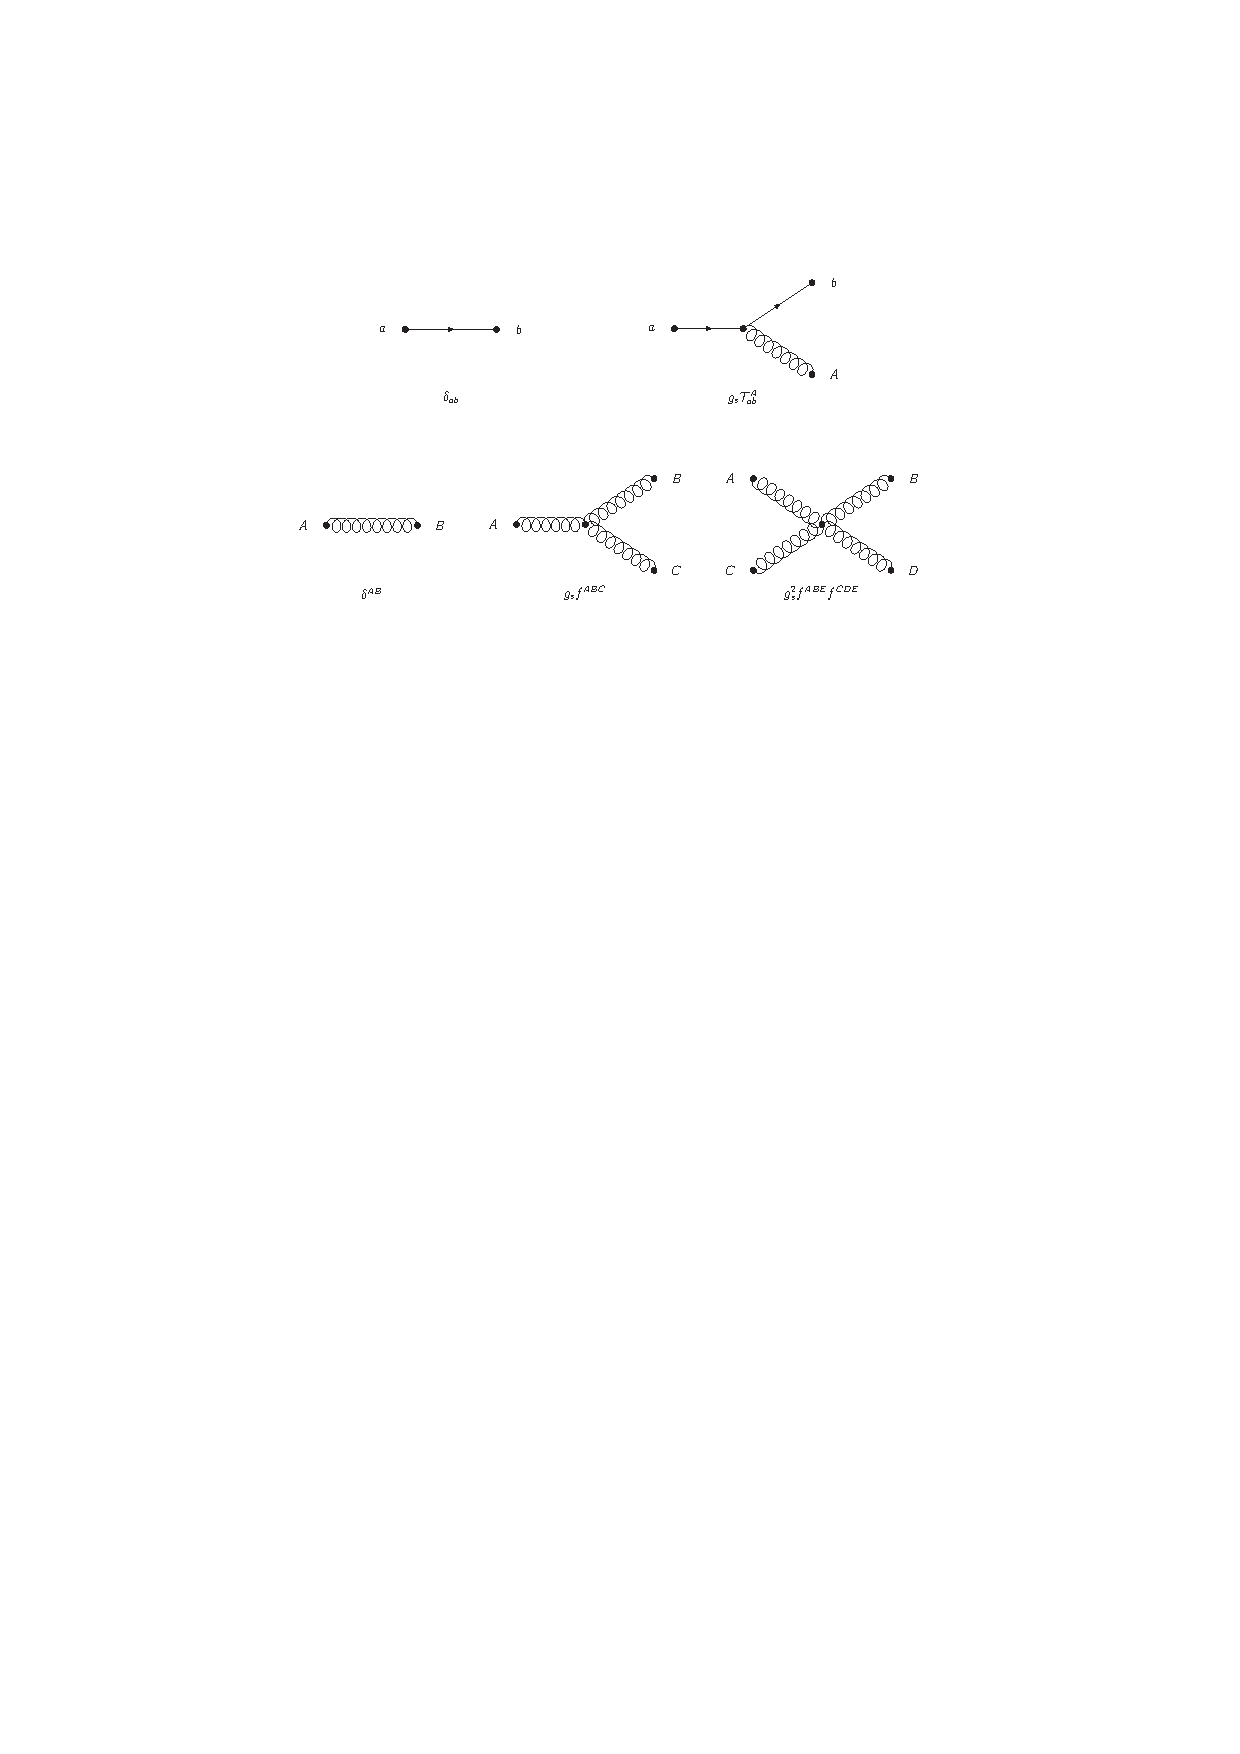
\includegraphics[width=0.95\textwidth]{/home/anter/Desktop/Thesis/Figures/edited_cropped_Feynmann.pdf}\\
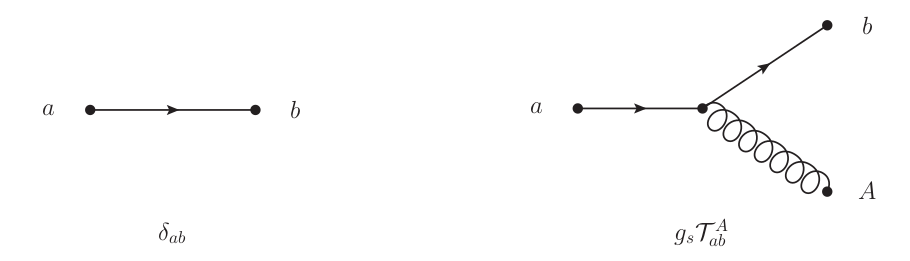
\includegraphics[width=0.8\textwidth]{/home/anter/Desktop/Thesis/Figures/Final/Feynman_1.png}\\
\vspace*{10mm}
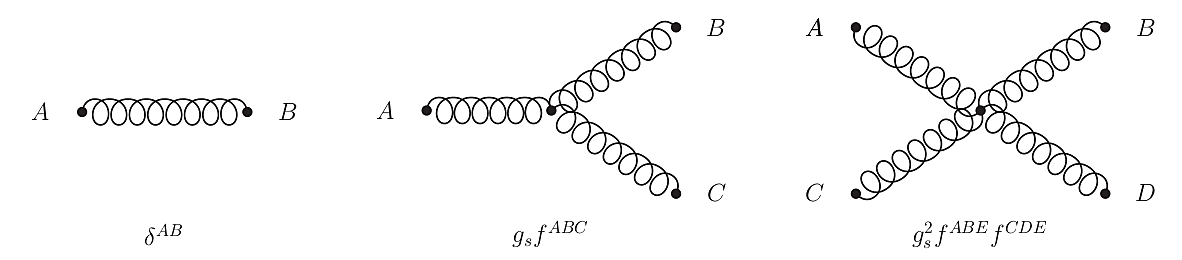
\includegraphics[width=0.95\textwidth]{/home/anter/Desktop/Thesis/Figures/Final/Feynman_2.png}
\vspace*{4mm}
\caption[The fundamental Feynman rules for different processes of quantum chromodynamics.]{The fundamental Feynman rules of a free quark-field term (top left), quark-gluon interaction term (top right), free gluon-field term (bottom left), cubic gluon self-interaction term (bottom middle) and quartic gluon self-interaction term (bottom right). Taken from \cite{Rabbertz:2017ssq}.}
\label{fig:feyn}
\end{center}
\end{figure}

It is impossible to use perturbation theory on a gauge invariant Lagrangian without choosing a specific gauge in which to calculate. The usual gauge-fixing term is given by 
\begin{equation}
{\cal L}_{gauge}=-\frac{1}{2\xi} (\partial^{\mu}{\cal A}^{A}_{\mu})^{2}
\label{eq:gauge-fixing}
\end{equation}
where $\xi$ may be any finite constant. This choice fixes the class of covariant gauges with $\xi$ as the gauge parameter. As QCD is non-abelian, the gauge fixing term must be supplemented by a ghost Lagrangian as
\begin{equation}
{\cal L}_{ghost}=\partial_{\alpha}\eta^{A\dagger}(D^{\mu}_{AB}\eta^{B})
\label{eq:ghost}
\end{equation}
where $\eta^{A}$ is a complex scalar field which obeys Fermi-Dirac statistics. The ghost fields cancel unphysical degrees of freedom arising due to use of covariant gauges. This completes the QCD Lagrangian shown in Eq.~\ref{eq:lag}.

The strength of an interaction is given by a fundamental parameter called the coupling constant $\alpha$. The electromagnetic coupling constant $\alpha_e$ = $e^2/4\pi$, the weak coupling constant $\alpha_w$ = $g^2_w/4\pi$ and the strong coupling constant \alpsq = $g^2_s/4\pi$ are not constant and each depends on the separation between the interacting particles. In contrast to $\alpha_e$, \alpsq increases with the increase in the distance or decrease in the energy scale $Q$, as shown in Fig.~\ref{fig:Grifiths}. $\alpha_w$ also increases with the increase in the distance but at a slower rate. At large distances or low energies, the quarks can never be found as free particles but exist in color neutral bound states known as hadrons. Hadrons are of two types : baryons and mesons. According to the quark model \cite{Griffiths:111880} every (anti-)baryon is made up of three (anti-)quarks and every meson is made up of a quark-antiquark pair. When the colored partons within a hadron are pulled farther and farther apart, there is an increase in the strength of force between them. This results in creation of new quark-antiquark pairs making it impossible to liberate a free quark or gluon. This property of QCD is known as confinement according to which at low energy, the partons are forever bound into hadrons such as protons ($uud$), neutrons ($udd$) etc. Although the gluons are massless, the confinement leads to the finite range of the strong interactions. On the other hand, at small distances, the strength of coupling decreases. The quarks and gluons interact very weakly and behave as free particles. This property is known as asymptotic freedom. This indicates that perturbative theory is only applicable at high energies or small distances.

\begin{figure}[!h]
\begin{center}
%\hspace*{-1.3mm}
%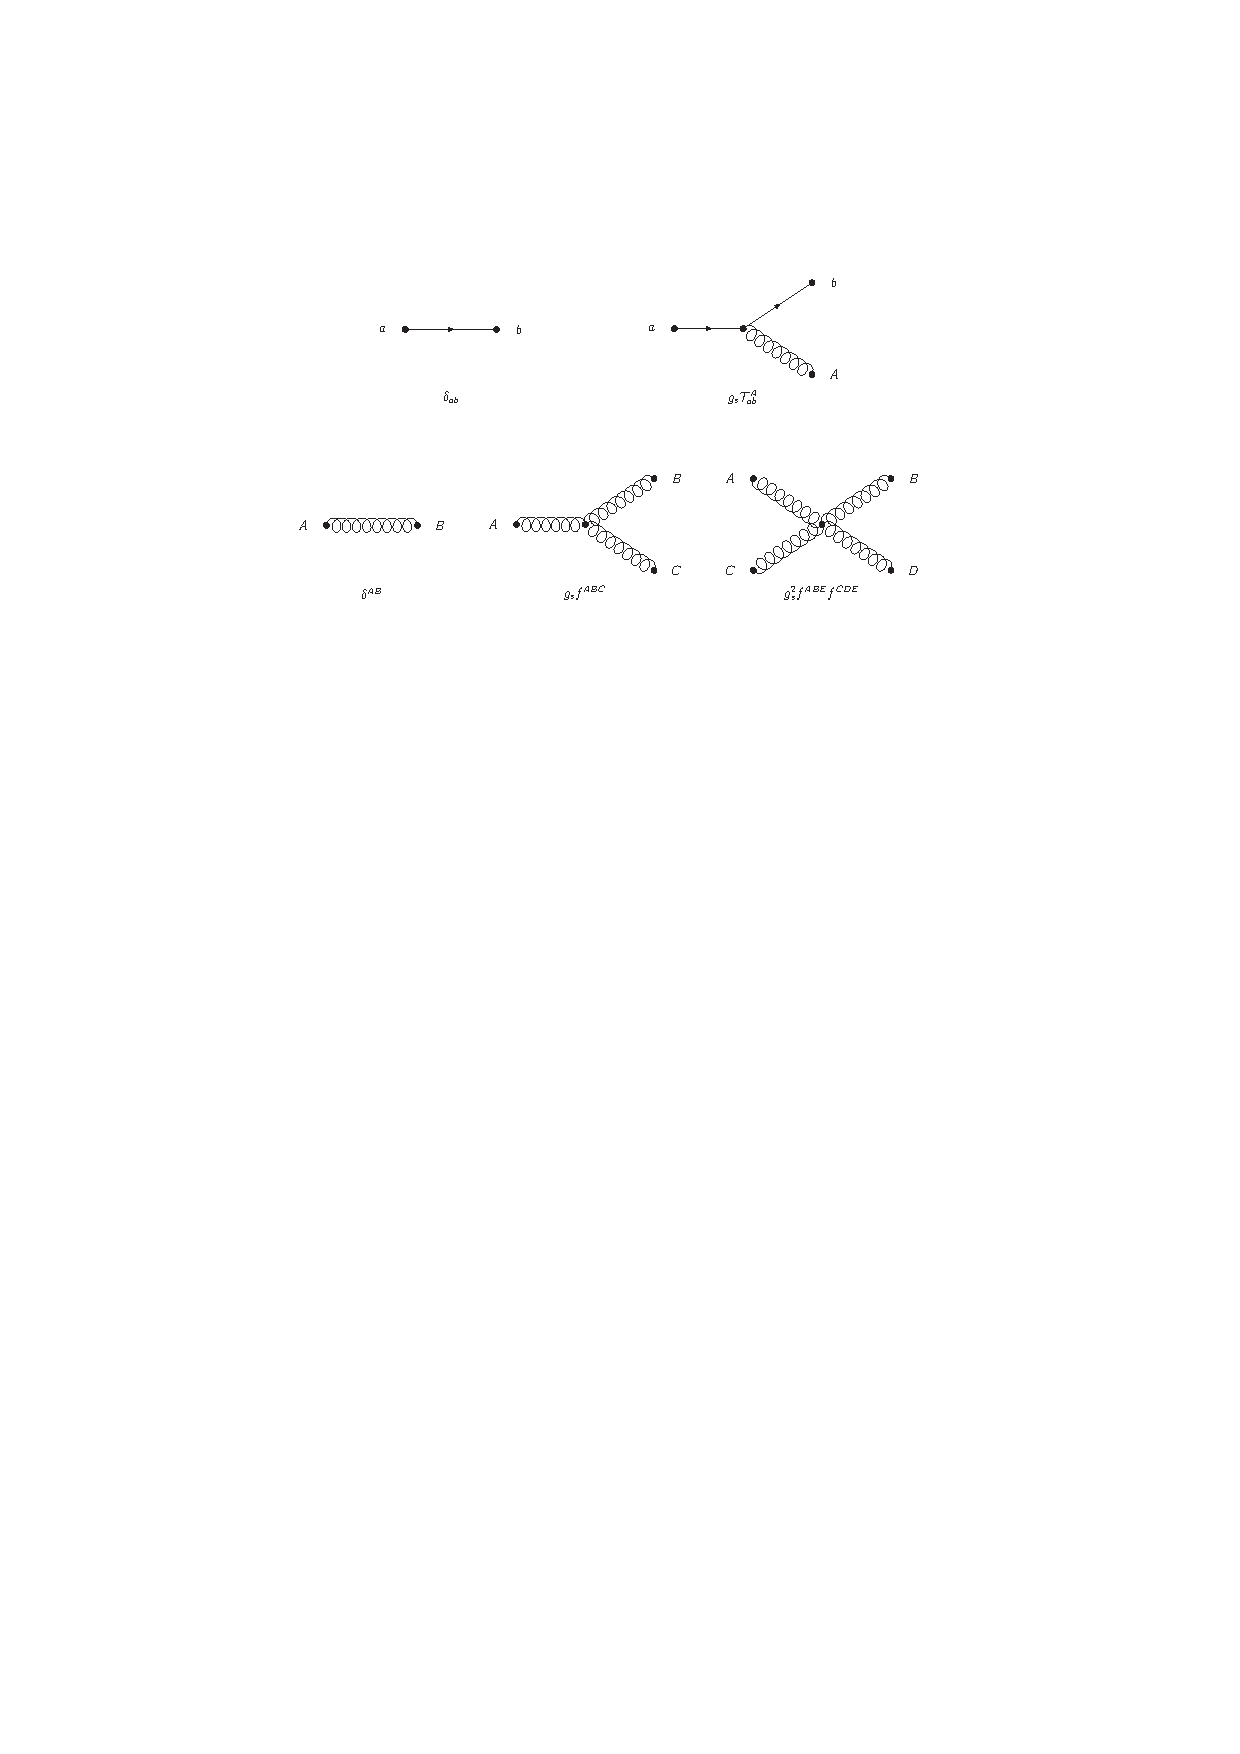
\includegraphics[width=0.95\textwidth]{/home/anter/Desktop/Thesis/Figures/edited_cropped_Feynmann.pdf}\\
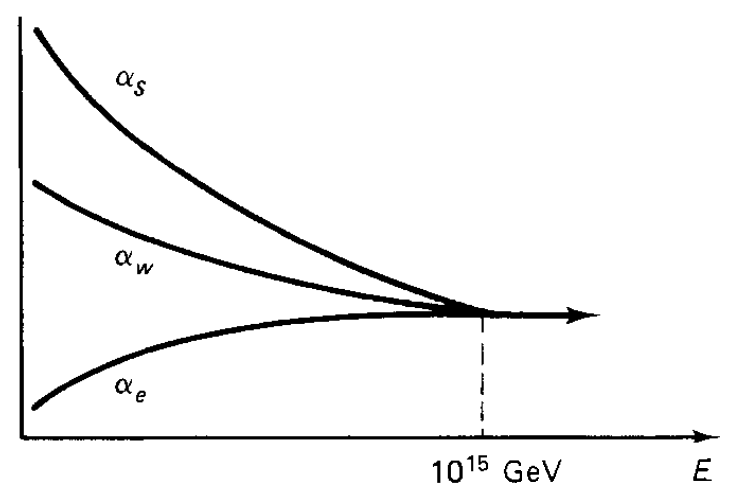
\includegraphics[width=0.5\textwidth]{/home/anter/Desktop/Thesis/Figures/Final/Grifiths.png}\\
\vspace*{4mm}
\caption[Evolution of three fundamental coupling constants : the strong coupling constant \alps, the weak coupling constant $\alpha_w$ and the electromagnetic coupling constant $\alpha_e$.]{Evolution of three fundamental coupling constants : the strong coupling constant \alps, the weak coupling constant $\alpha_w$ and the electromagnetic coupling constant $\alpha_e$. Taken from \cite{Griffiths:111880}.}
\label{fig:Grifiths}
\end{center}
\end{figure}

\subsection{Perturbative Quantum Chromodynamics}
At high energies, the property of asymptotic freedom allows a perturbative treatment in QCD calculations. In perturbative quantum chromodynamics (pQCD), a physical observable $X$ such as cross-section of a scattering process, can be expanded as a perturbative series in terms of coupling constant \alps as : 
\begin{equation}
\label{eq:pertur}
X = \sum\limits_{i=0}^{N} \alpha^n_s {\rm c}_i = {\rm c}_0~\plus \alpha^1_s {\rm c}_1~\plus \alpha^2_s {\rm c}_2~\plus ...
\end{equation} 
where ${\rm c}_i$ are the perturbative coefficients. In a process, the pQCD calculation of X is determined by summing over the amplitudes of all Feynman diagrams contributing to that process. For a given Feynman diagram, the power of \alps is determined by the number of vertices associated with quark-gluon or gluon-gluon interactions. A leading order (LO) prediction sums over only the lowest-order contribution whereas next-to-leading order (NLO) includes terms with one additional power of \alps. The next-to-next-to-leading order (NNLO) includes emission of another gluon or a virtual gluon loop. The different orders in a 2 $\rightarrow$ 2 scattering process are shown in Fig.~\ref{fig:orders}. The calculations become complex with the loop diagrams where the momenta of the virtual particles in a loop are not fully constrained by four-momentum conservation and the associated integrals are divergent. Such ultraviolet (UV) divergences enter the calculations beyond LO either due to loop or vertex corrections. These are overcome by a procedure known as renormalization, described in next section. Apart from the UV divergences, the QCD also suffers from infrared and collinear divergences (IRC) due to the presence of massless gluons and neglected quark masses. These need to be handled in pQCD calculations. The observable to be studied must be IRC safe. 

\begin{figure}[!h]
\begin{center}
\vspace*{2mm}
\hspace*{-8mm}
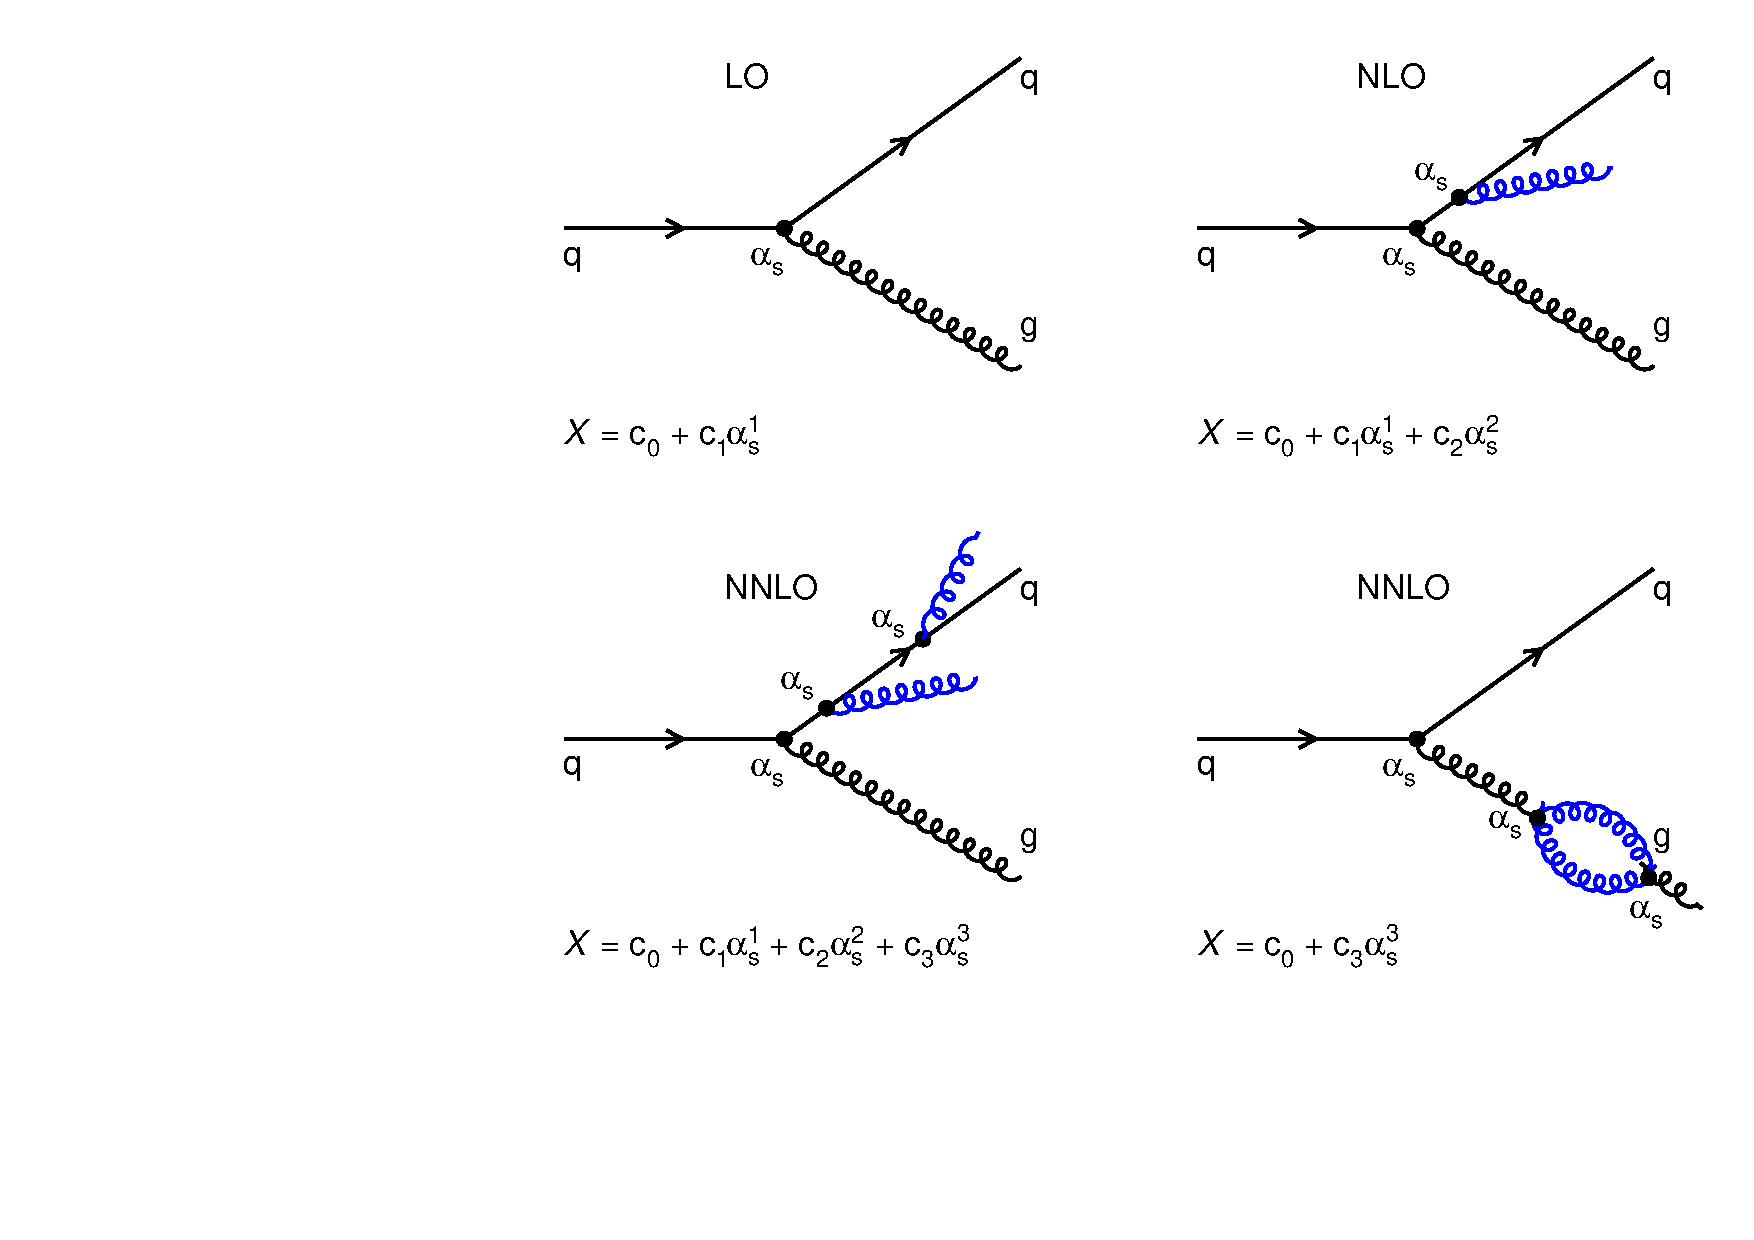
\includegraphics[width=1.1\textwidth]{/home/anter/Desktop/Thesis/Figures/Orders.pdf}\\
\vspace*{4mm}
\caption[Feynman diagrams of leading-order (LO), next-to-leading order (NLO) and next-to-next-to-leading order (NNLO) processes in quantum chromodynamics.]{Feynman diagrams\footnotemark of leading-order (LO), next-to-leading order (NLO) and next-to-next-to-leading order (NNLO) contributions of 2 $\rightarrow$ 2 scattering process.}%At each successive step in perturbation series, the emission of an additional gluon take place.}
\label{fig:orders}
\end{center}
\end{figure}

\subsection{Renormalization and Running of the Strong Coupling}
The renormalization is a mathematical procedure which allows the finite calculation of momenta integrals of virtual loop by removing UV divergences. It introduces a regulator for the infinities, the renormalization scale \mur. At first, the divergences are regularized temporarily by introducing a cut-off to the loop momenta at \mur scale. Then the free parameters of the Lagrangian, i.e. the coupling constant are redefined or renormalized to absorb the UV divergences.\footnotetext{Drawn using ROOT} Due to this, both \alpsq and observable $X$ become a function of \mur. The exact dependence of \alpsmusq on \mur is described by the renormalization group equation (RGE) \cite{Callan:1970yg} which determines the running of \alpsmusq. According to RGE, the dependence of $X$ on \mur must cancel. Mathematically this can be expressed as :
 
\begin{equation}
\mur^{2}\frac{d}{d\mur^{2}}X\Bigg(\frac{Q^{2}}{\mur^{2}},\alpha_{s}(\mur^{2})\Bigg)=
\Bigg(\mur^{2}\frac{\partial}{\partial\mur^{2}}~\plus \mur^{2}\frac{\partial\alpha_{s}(\mur^{2})}
{\partial\mur^{2}}\frac{\partial}{\partial\alpha_{s}(\mur^{2})}\Bigg)X=0
\label{eq:dmu}
\end{equation}
Using beta function $\beta(\alps)$ = $\mur^{2}\frac{\partial\alpha_{s}(\mur^{2})}{\partial\mur^{2}}$, Eq.~\ref{eq:dmu} can be re-written as 
\begin{equation}
\Bigg(\mur^{2}\frac{\partial}{\partial\mur^{2}}~\plus \beta(\alps)\frac{\partial}{\partial\alpha_{s}(\mur^{2})}\Bigg)X=0
\label{eq:dmu2}
\end{equation}
By setting the renormalization scale equal to the physical scale i.e. $\mu^{2}=Q^{2}$, $X\big(1,\alpha_{s}(Q)\big)$ is a solution to above equation where $Q$-dependence of $X$ is only from the renormalization of the theory. Hence measuring the $Q$-dependence of $X$ will directly probe the quantum structure of the theory. The $\beta$ function in QCD has a perturbative expansion as : 
\begin{equation}
\beta(\alps)=-\alpha_{s}^{2}\Big(b_0~\plus b_1\alps~\plus b_2\alpha_{s}^{2}~\plus {\cal O}(\alpha_{s}^{3})\Big) 
\label{eq:beta}
\end{equation}
where $b_n$ is the $n$\plus 1-loop $\beta$-function coefficients giving the dependence of the coupling on the energy scale $Q$. In the modified minimal subtraction ($\overline{\rm MS}$) scheme \cite{tHooft:1973mfk,Weinberg:1951ss}, the beta coefficient functions have following values :
\begin{equation}
b_0 = \frac{33-2n_f}{12\pi}, ~~~b_1 = \frac{153-19n_f}{24\pi^2}, ~~b_2 = \frac{77139 - 15099n_f~\plus 325n^2_f}{3456\pi^3}
\end{equation}
where $n_f$ is the number of quark flavors with masses $m_q$ \ls \mur. On integration of Eq.~\ref{eq:beta}, the energy dependence of \alps is yielded. Neglecting the higher orders, the first order solution of RGE is :
\begin{equation}
\alpha_{s}(\mur^2)=\frac{1}{b_0~{\rm ln}(\mur^2/\Lambda^2_{QCD})}
\label{eq:sol}
\end{equation}
where $\Lambda_{QCD}$ is the constant of integration. The perturbative coupling becomes large at the scale $\Lambda_{QCD}$ and the perturbative series diverge. With $b_0$ \gr 0, the coupling becomes weaker at higher scales $Q$, i.e. the effective color charge is small at small distances or large energies. This allows the quarks to behave as free particles within the hadron, leading to the property called asymptotic freedom. It is always convenient to express \alps at some fixed scale. Since some of the best measurements come from $Z$ decays, it is common practice to determine the strong coupling at the scale of the $Z$ boson mass \alpsmz. So, Eq.~\ref{eq:sol} can be expressed as :
\begin{equation}
\alps\bigg(\mur,\alpsmz\bigg) = \frac{\alpsmz}{1\plus\alpsmz b_0{\rm ln}(\mur^2/M^2_z)}
\end{equation}

Since \alps is a free parameter of QCD theory, it must be extracted from experimental measurements and evolved to the scale of the $Z$ boson. According to Particle Data Group (PDG) \cite{Patrignani:2016xqp}, the current world average value of the strong coupling constant at the scale of mass of $Z$ boson is 
\begin{equation}
\alpsmz = 0.1181 \pm 0.0011
\end{equation}
This value is derived using data from deep inelastic scattering process, electron-positron annihilation processes, hadronic $\tau$ lepton decays, lattice QCD calculations and electroweak precision fits. The different experimental determinations of the strong coupling constant evolved at the scale $Q$ are shown as a function of $Q$ in Fig.~\ref{fig:alpha_pdg} which describe the running of the \alps up to the 1 TeV scale.
\vspace*{2mm}
\begin{figure}[!h]
\begin{center}
\hspace*{-7mm}
%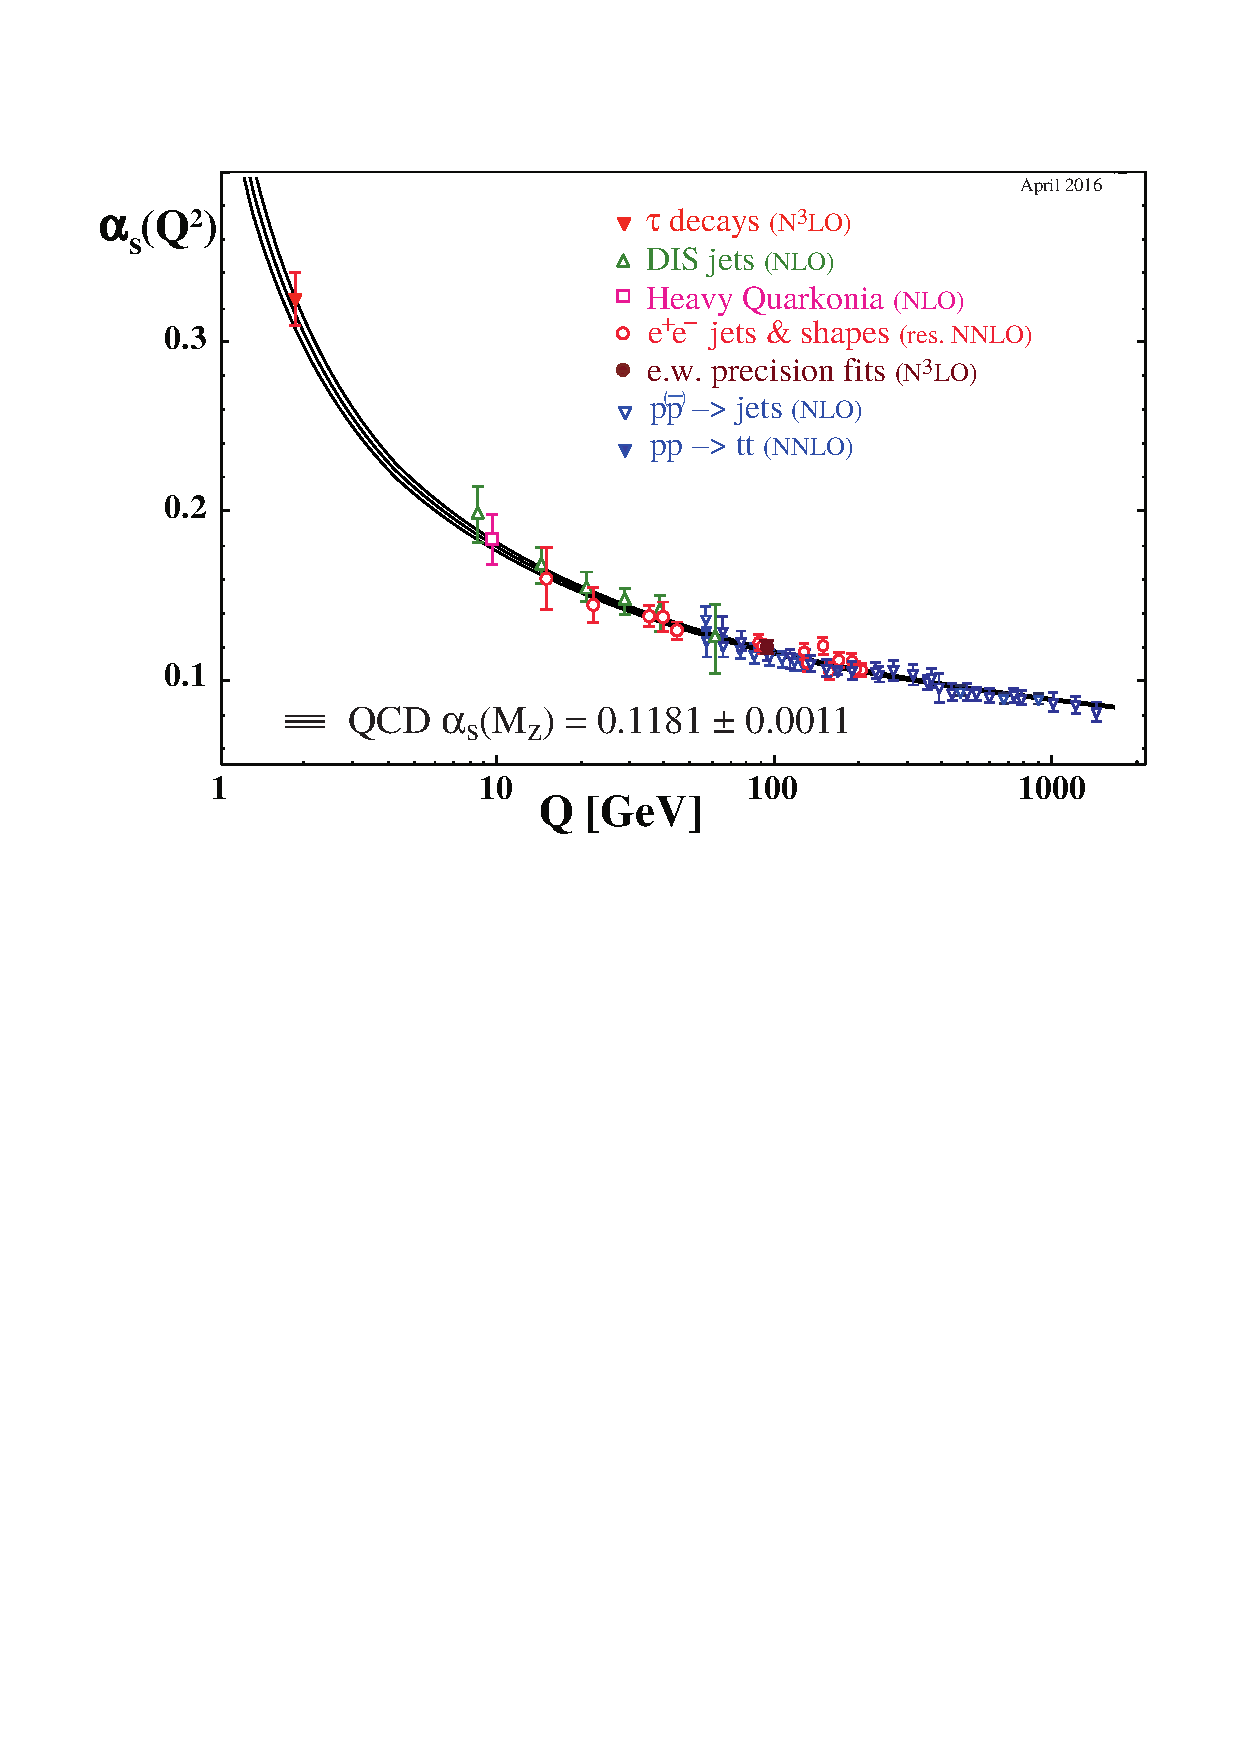
\includegraphics[width=0.95\textwidth]{/home/anter/Desktop/Thesis/Figures/cropped_Alpha.pdf}\\
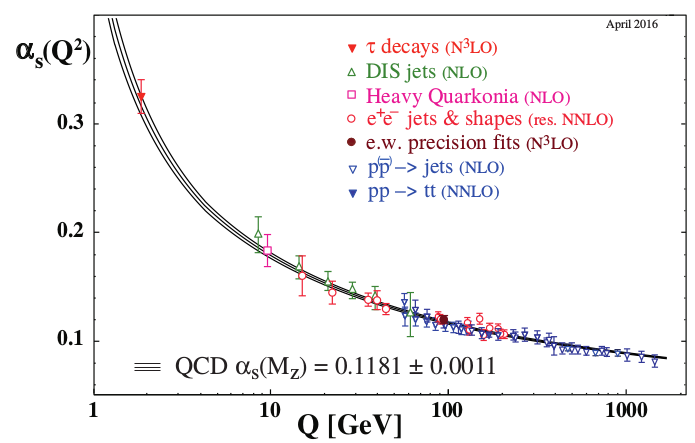
\includegraphics[width=0.95\textwidth]{/home/anter/Desktop/Thesis/Figures/Final/Alpha.png}\\
\vspace*{4mm}
\caption[Running of the strong coupling constant evolved at the energy scale $Q$ as a function of $Q$.]{Different experimental determinations of the strong coupling constant \alps evolved at the energy scale $Q$ are shown as a function of $Q$. These describe the running of the \alps up to the 1 TeV scale. Taken from \cite{Patrignani:2016xqp}.}
\label{fig:alpha_pdg}
\end{center}
\end{figure}

\section{Hadronic Collisions}
At large momentum transfer, the collision between two hadrons can be visualized as an interaction between their constituents - quarks and gluons. In this thesis, we are studying the proton-proton collisions taking place at the Large Hadron Collider (LHC). A proton is a complex composite particle consisting of three valence quarks ($uud$), gluons for the exchange of the strong force and the sea quarks. The sea quarks consist of quark-antiquark pairs coming into and out of existence rapidly and continuously due to gluon color field splitting. In any collision, a fundamental quantity to evaluate is the cross-section ($\sigma$) of a certain process which gives the probability that the two hadrons interact and give rise to that final state. In a hadronic collision, the perturbation theory is only valid at the parton-level but due to property of confinement at low energies, free partons cannot exist in nature. Only colorless hadrons can emerge as free particles from the high energy collisions. Here, the factorization theorem of QCD \cite{Collins:1989gx} comes into play which allows the calculation of $\sigma$ by separating into two parts : a short-distance partonic cross-section calculable with pQCD, and a non-perturbative long-distance part described by parton distribution functions $f_i(x,\muf)$ (PDFs). The PDFs describe the partonic content of the colliding hadrons and give the probability to find a parton $i$ with momentum fraction $x$ within a hadron. \muf is the factorization scale which corresponds to the resolution with which the hadron is being probed. The particles which are emitted with transverse momenta \pt \gr \muf are considered in the calculation of hard scattering perturbative coefficients. The particles emitted with \pt \ls \muf are accounted for within the PDFs. Applying the factorization theorem to a proton-proton collision, the cross-section of a hard scattering process can be written as :

\begin{equation}
\begin{gathered}
\sigma_{P_1P_2 \rightarrow X} = \sum\limits_{i,j}^{}\int_{}^{} dx_1dx_2f_{i,P_1}(x_1,\muf)f_{j,P_2}(x_2,\muf)\\\times~\hat\sigma_{ij\rightarrow X} \Bigg(x_1p_1,x_2p_2,\alpha(\mur^2),\frac{Q^2}{\muf^2}\Bigg)
\end{gathered}
\end{equation}
where $f_i$ and $f_{j}$ are the proton PDFs which depend on momentum fractions $x_1$ and $x_2$ of parent protons $P_1$ and $P_2$ respectively as well as on the factorization scale \muf. The sum extends over all contributing initial-state parton flavors $i,~j$. The cross-section for the production of final state $X$ at parton level ($\hat\sigma_{ij}$) depends on the final state phase space, the factorization scale \muf and the renormalization scale \mur. Figure~\ref{fig:fac} illustrates the factorization into the PDFs and the hard scattering cross-section in a proton-proton collision.
\begin{figure}[!h]
\begin{center}
\hspace*{-7mm}
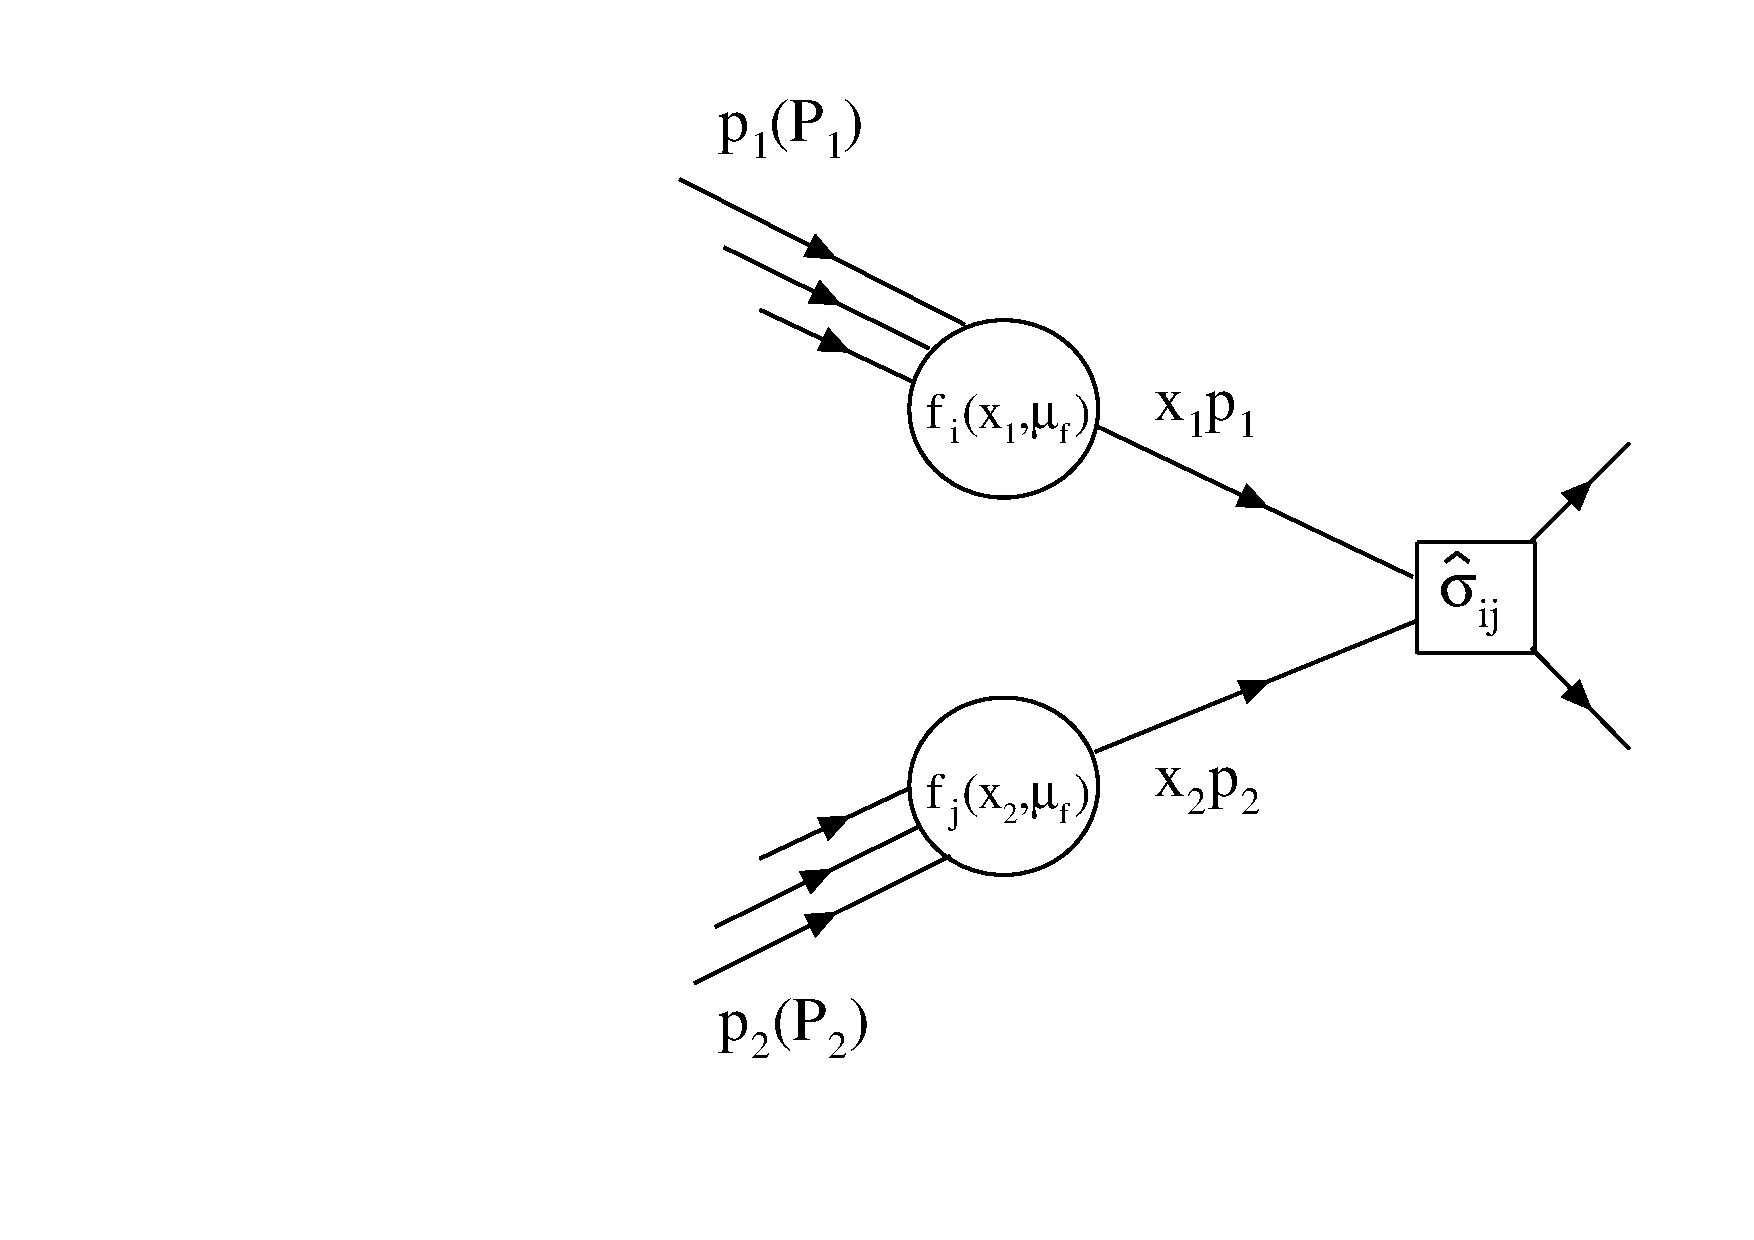
\includegraphics[width=0.65\textwidth]{/home/anter/Desktop/Thesis/Figures/Factorization.pdf}\\
\vspace*{4mm}
\caption[Schematic illustration of the factorization theorem in a collision of two protons.]{Schematic illustration\footnotemark of the factorization theorem in a collision of two protons P1 and P2 having momenta p1 and p2, respectively. In a hard-scattering process at a scale $Q^2$, the two partons $x_1$ and $x_2$ participate with momenta $x_1p_1$ and $x_2p_2$. The total cross-section is factorized into the hard scattering cross-section $\hat\sigma_{ij}$ calculable using pQCD and the PDFs $f_i(x_1,\muf)$ and $f_j(x_2,\muf)$ with factorization scale \muf.}
\label{fig:fac}
\end{center}
\end{figure}

The PDFs of the proton are a necessary input to almost all theory predictions of a proton-proton collision. Perturbative QCD does not predict the parton content of the proton. So the shapes of PDFs are determined in fits to experimental measurements of different experiments. The dependence of PDFs on \muf is given by the Dokshitzer-Gribov-Lipatov-Altarelli-Parisi (DGLAP) \cite{Gribov:1972ri,Dokshitzer:1977sg,Altarelli:1977zs} equations which use \alps and the RGE as inputs. The knowledge of proton PDFs mainly comes from Deep-Inelastic-Scattering (DIS) HERA, fixed target and Tevatron data. The LHC data have a potential to improve constraints of the PDFs further as done in one of the recent CMS measurements \cite{Sirunyan:2017skj}. There are several groups which determine the PDFs which mainly differ in choice of input data sets, treatment of heavy quarks, order of perturbation theory, way of treating experimental errors and theoretical assumptions. Global PDFs are the CTEQ \cite{Dulat:2015mca}, MMHT \cite{Harland-Lang:2014zoa}, NNPDF \cite{Ball:2014uwa} and ABM \cite{Alekhin:2012ig} at LO, NLO and NNLO.%using the different minimization methods, phenomenological approaches and the methods to estimate the uncertainties. and HERAPDF \cite{Abramowicz:2015mha} 
%Source : \url{https://arxiv.org/pdf/1003.0521.pdf}}

\subsection{Parton Shower and Hadronization}
\footnotetext{Drawn using ROOT}
The partons involved in a hard scattering process get accelerated due to large momentum transfers. These accelerated partons emit QCD radiation in the form of gluons with successively lower energy. Unlike the uncharged photons in QED, the gluons themselves carry color charge and hence emit further gluons. The emitted gluons in turn can split into $q\bar{q}$ pairs. This successive emission of partons is described as a parton shower. In a parton shower, the main contribution is by the collinear parton splitting and the soft gluon emissions. The parton showers mimic the effect of higher-order corrections to the hard process. These cannot be calculated exactly and are taken into account using the parton shower approximation. The two incoming partons, which are constituents of two colliding hadrons and take part in hard scattering process, can also develop parton showers, commonly known as Initial-State Radiation (ISR). The initial partons produce showers till they collide to initiate the hard scattering process. The final outgoing partons produced from a hard scattering process can also undergo parton showering giving rise to Final-State Radiation (FSR). A parton shower terminates when the scale $Q$ is below the hadronization scale $\sim$ 1 GeV for QCD.

At the end of the shower, there is a decrease in the energy of partons due to successive emission of gluons. Due to this, the coupling constant of QCD \alps grows large and pQCD is not applicable anymore. This leads to the confinement of colored quarks and gluons into the color-neutral composite particles called hadrons and this process is known as hadronization. The hadronization takes place at low momentum transfer and hence is non-perturbative in nature. Because no exact theory for hadronization is known, different phenomenological models have been developed to simulate the hadronization process. The two main models implemented in Monte Carlo (MC) event generators are : \\\newline
{\bf Lund String Fragmentation Model -} In the Lund string model of hadronization \cite{Andersson:1998tv}, the highly energetic gluons are treated as field lines. Due to the gluon self-interaction, the gluons are attracted to each other forming a narrow tube or string of strong color field between a $q\bar{q}$ pair. This model is based on an observation that at distances greater than about a femtometre (fm)\footnote{~~1 femtometre = 1$\times$ 10$^{-15}$ metres}, the potential energy $V(r)$ of colored quarks grows linearly with the increase in distance between them ($r$) as :
\begin{equation}
V(r) = \kappa r
\end{equation}
where $\kappa \sim 1~{\rm GeV/fm}$ is the tension of the string connecting the quarks. When the $q$ and $\bar{q}$ are pulled apart from each other, the gluonic string stretches. As a consequence, the potential energy of the string grows at the expense of the kinetic energy of the quarks. As the potential energy approaches the order of hadron masses, the string breaks at some point along its length, creating a new $q\bar{q}$ pair. The newly formed two string segments again stretch and break producing further $q\bar{q}$ pairs. This process of stretching and breaking continues until all the potential energy gets converted to $q\bar{q}$ pairs. This whole process is illustrated in Fig.~\ref{fig:string}. Subsequently, the $q\bar{q}$ pairs are transformed into final-state hadrons. The \PYTHIA~MC generator uses the Lund string fragmentation model. 
\begin{figure}[!h]
\begin{center}
\hspace*{-4mm}
%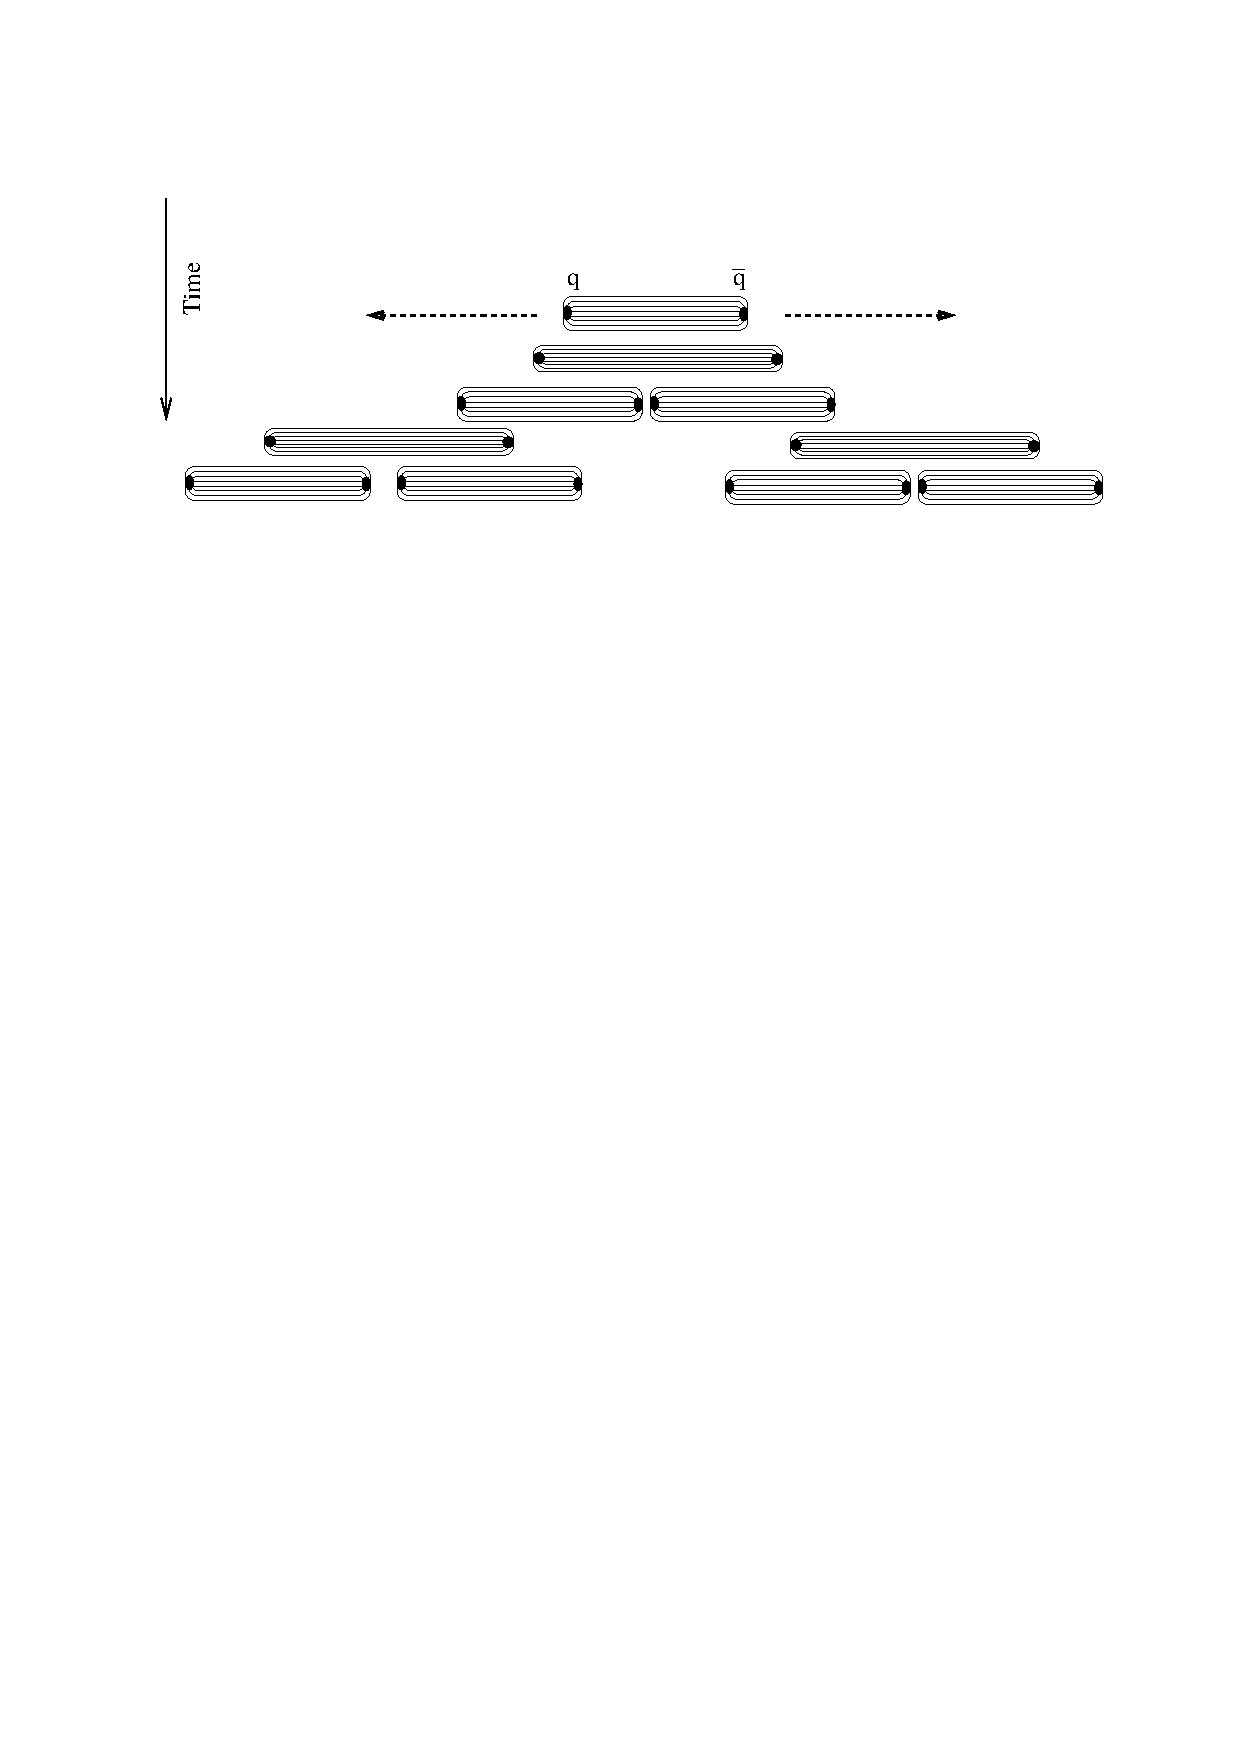
\includegraphics[width=0.95\textwidth]{/home/anter/Desktop/Thesis/Figures/cropped_String.pdf}\\
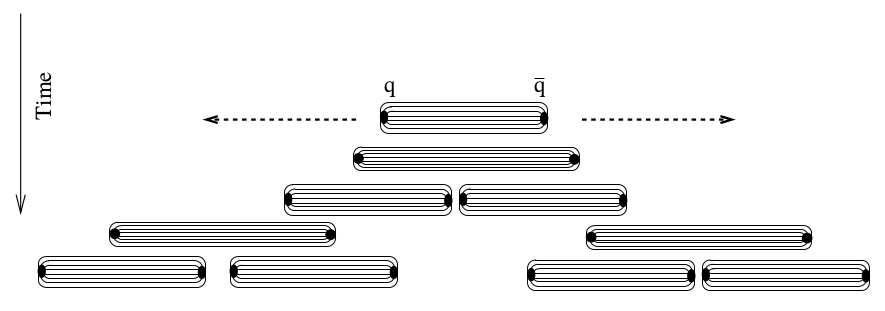
\includegraphics[width=0.95\textwidth]{/home/anter/Desktop/Thesis/Figures/Final/String.png}\\
\vspace*{4mm}
\caption[Illustration of the hadronization process in Lund string model.]{Illustration of the hadronization process in Lund string model\footnotemark. When the quark $q$ and anti-quark $\bar{q}$ are pulled apart from each other, the potential energy of the gluonic string connecting the quarks increases. As it becomes of the order of hadron masses, the string breaks and a new $q\bar{q}$ pair is created. The breaking of string and creation of $q\bar{q}$ continues till all the potential energy gets converted to $q\bar{q}$ pairs which then get hadronized.}
\label{fig:string}
\end{center}
\end{figure} \\
{\bf Cluster Fragmentation  Model -} \footnotetext{Source : \url{http://inspirehep.net/record/806744}}The cluster model of hadronization \cite{Marchesini:1987cf,Webber:1983if} is based on preconfinement property of QCD \cite{Amati:1979fg}. According to this property, at evolution scales $Q_0$ much less than the hard process scale $Q$, the partons produced in a shower are clustered in colorless groups with an invariant mass distribution, depending on nature of hard process and $Q_0$, not on $Q$. This model contains two steps : firstly all gluons split into $q\bar{q}$ pairs at the end of the parton shower and in the second step, a new set of low-mass color-singlet clusters are obtained which decay into either secondary clusters or directly into hadrons. The generator \HERWIG~is based on the cluster fragmentation model. %However, this model has problems in dealing with the decay of very massive clusters. 

\subsection{Underlying Event}
Due to the composite nature of the protons, the event structure is significantly more complex than that of the lepton collisions. The final states of the collisions involve multi-parton interactions. In a high energy proton-proton collisions, the underlying event (UE) includes the effects which are not coming from the primary hard scattering process. \begin{figure}[!h]
\begin{center}
\hspace*{-7mm}
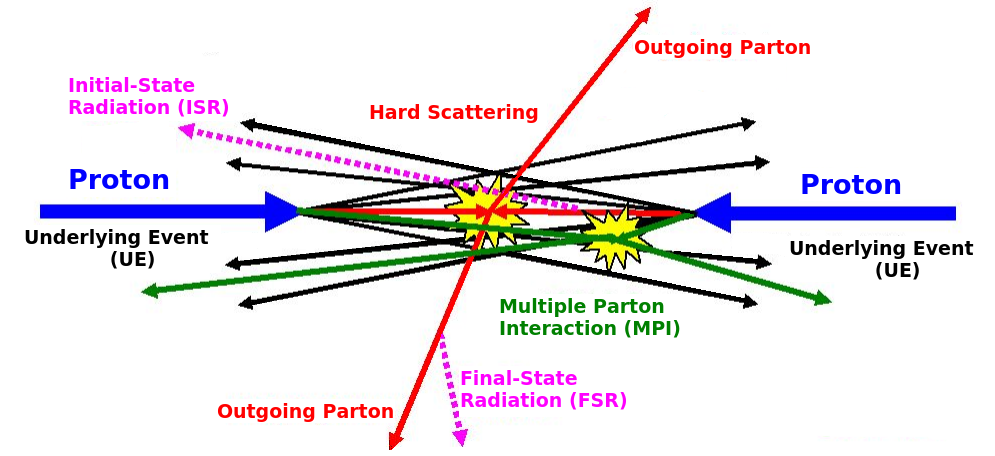
\includegraphics[width=0.98\textwidth]{/home/anter/Desktop/Thesis/Figures/MPI.png}\\
\vspace*{4mm}
\caption[A proton-proton collision involving the main hard scattering process along with the low momentum transfer underlying event (UE) contributions.]{A proton-proton collision\footnotemark~involving the main hard scattering process along with the low momentum transfer underlying event (UE) contributions coming from initial- and final-state radiations (ISR and FSR) complemented with multiple parton interactions (MPI) and collisions from leftover partons called beam remnants.}
\label{fig:MPI}
\end{center}
\end{figure}\footnotetext{Source : \url{https://cds.cern.ch/record/1382404}}The UE includes the contributions from relatively small momentum transfer processes : initial and final-state radiations (ISR, FSR), leftover partons in the collisions called beam remnants and multiple parton interactions (MPI). Due to composite nature of proton, the remaining two partons which do not participate in a hard collision may also interact giving rise to multiple parton interactions. The UE induces an additional energy in an event which is not related to the main interaction. This acts as an unavoidable background which needs to be removed. Hence, it is crucial to study and understand the UE. The UE activity increases with $Q$ and the center-of-mass energy \cme. Figure~\ref{fig:MPI} shows the complex variety of processes taking place in a single proton-proton collision.

\section{Jets}
\label{sec:jets}
The bunch of hadrons, produced from hadronization of quarks and gluons, gets collimated in the form of ``jets'' with the direction towards the direction of the initial parton that originated them. The jets \cite{Sterman:1977wj} are conical structures which group hadrons into a single physics entity and can be observed experimentally in the detectors. These act as a bridge between the elementary quarks and gluons of QCD and the final hadrons produced in high energy collisions. The jet structure was observed for the first time in hadron production of $e^\plusn e^-$ annihilation process at SLAC in 1975 \cite{Hanson:1975fe}. Figure~\ref{fig:jet_r} shows the the outgoing partons of the hard scattering process in a proton-proton collision, undergoing fragmentation and hadronization processes and forming a conical jet with radius R. \\
\begin{figure}[!h]
\begin{center}
\hspace*{-7mm}
\vspace{2mm}
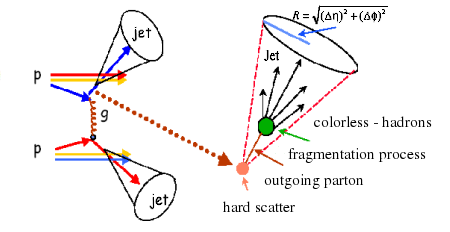
\includegraphics[width=0.75\textwidth]{/home/anter/Desktop/Thesis/Figures/jet2.png}\\
\vspace*{4mm}
\caption[Formation of a jet in a proton-proton collision.]{In a proton-proton collision, the outgoing partons of the hard scattering process undergo fragmentation and hadronization processes producing a shower of partons which get collimated into a conical jet with radius R.}
\label{fig:jet_r}
\end{center}
\end{figure}

The partons can not be measured directly by the experiments because they can not exist freely in nature. The information about the dynamics of the partons can be obtained indirectly from jets. The configurations of high-energy quarks and gluons at short distances are reflected in the energy and angular distributions of the jets. Hence, the jets are important to study. Therefore, at large momentum transfer of the interacting partons, the jets and their observables are the best tools to test the predictions of pQCD. Also, the jet production is sensitive to the strong coupling constant \alpsns. The precise knowledge of the jet production cross-section can help to extract the value of \alps and also to reduce the uncertainties of the PDFs of the proton. At the LHC, the simplest jet production process is a 2 $\rightarrow$ 2 scattering process giving dijet events, whereas 2 $\rightarrow$ 3, 2 $\rightarrow$ 4 parton reactions in pQCD give rise to multijet events. The investigation of inclusive multijet event cross-sections permits more elaborate tests of QCD. Also, a precise study of jet variables helps to understand the signal and background modelling for new physics searches in hadronic final states. In this thesis, the inclusive multijet event cross-sections as well as the ratio of cross-sections are exploited to extract the value of the strong coupling constant \alps. In the next section, we focus on the definition of a jet.%The partons originating from ISR, FSR or MPI can also hadronize to produce further jets within the same proton-proton collision. These UE events serve as background which are cut out selecting jets with high transvers. \gr 150 GeV is results in the production of multijet events. 

\subsection{Jet Algorithms}
\label{sec:jet_algos}
Jet algorithms \cite{Salam:2009jx} provide a set of rules which determine how the particles can be clustered into a jet. In a jet algorithm, usually one or more parameters are involved that indicate how close two particles must be for them to belong to the same jet. These parameters can either measure closeness in coordinate space (cone algorithms) or in momentum space (sequential recombination algorithms). The jet algorithms are applicable on parton, particle and detector levels. A recombination scheme is always associated with a jet algorithm which calculates the momentum assigned to the combined particles. A jet algorithm along with its parameters and a recombination scheme forms a ``jet definition''. A jet definition \cite{Ellis:1989vm} must be simple to implement in an experimental analysis as well as in the theoretical calculation. It should be defined at any order of perturbation theory and must yield finite cross-sections that are relatively insensitive to hadronization. In addition to these requirements, a jet algorithm must be infrared and collinear (IRC) safe. Infrared safety is the property by which the addition of a soft emission i.e. addition of a soft gluon should not change or modify the number of hard jets found in an event. In an infrared unsafe algorithm, a soft gluon emission in the middle of two cone jets can lead to overlap of the two initial cones, as shown in Fig.~\ref{fig:IRC} (top). 
\begin{figure}[h!]
\begin{center} 
%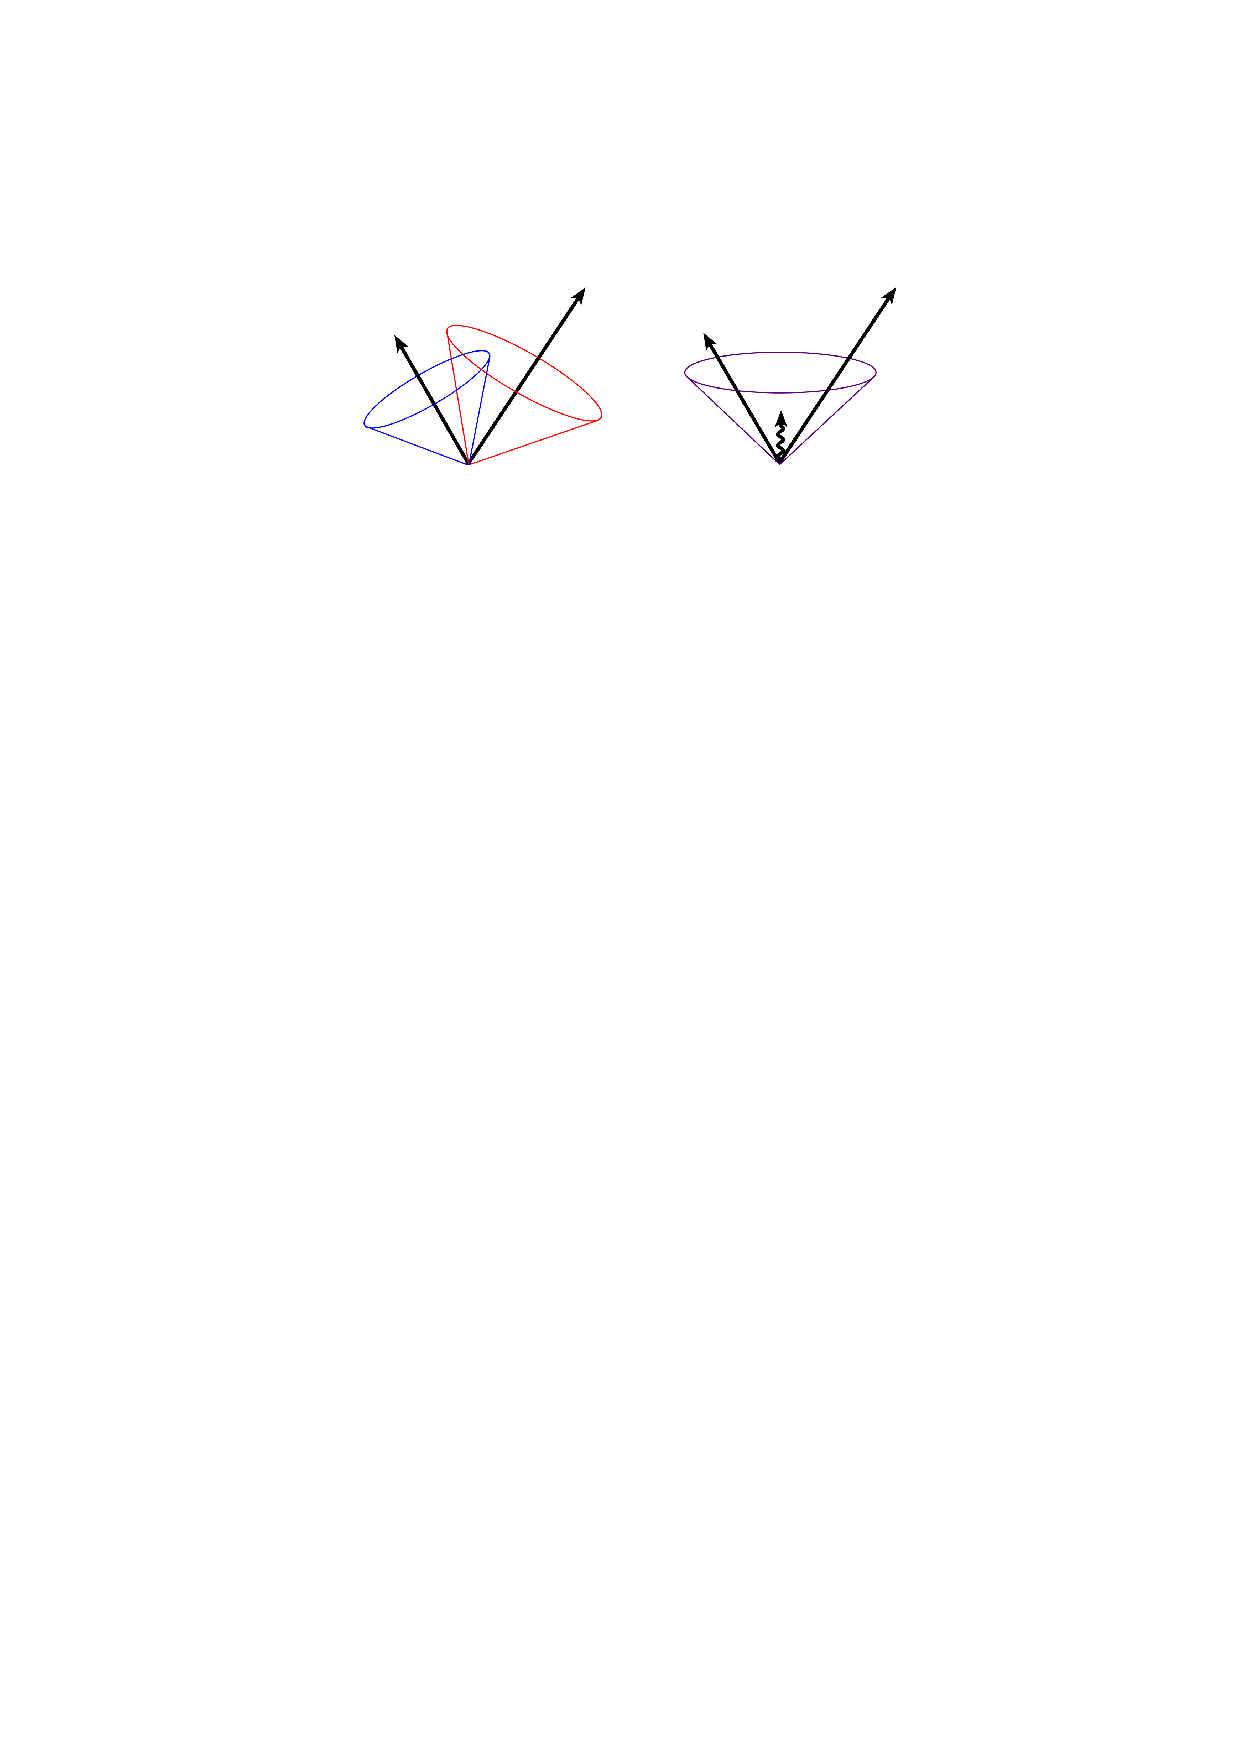
\includegraphics[scale = 1.3]{/home/anter/Desktop/Thesis/Figures/cropped_IR.pdf}\\
%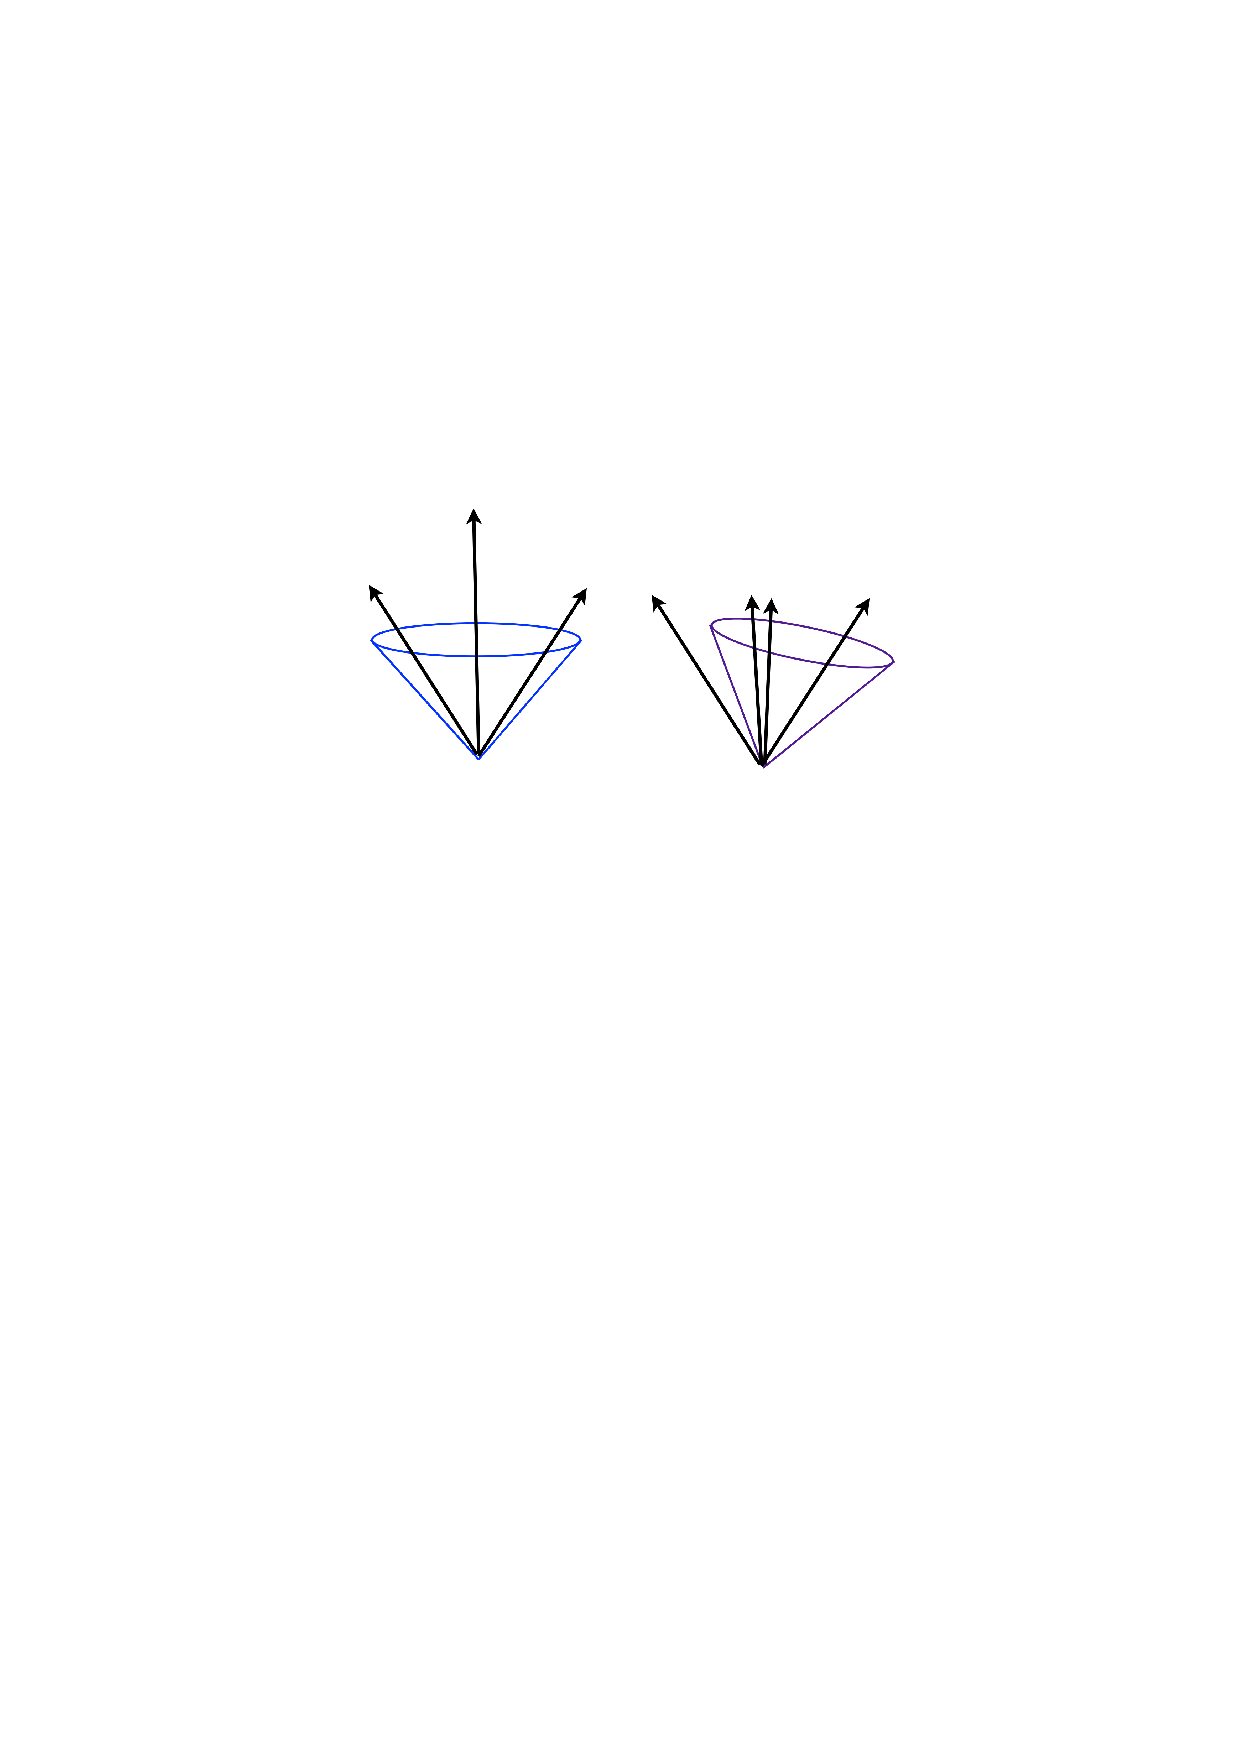
\includegraphics[scale = 1.1]{/home/anter/Desktop/Thesis/Figures/cropped_Collinear.pdf}
%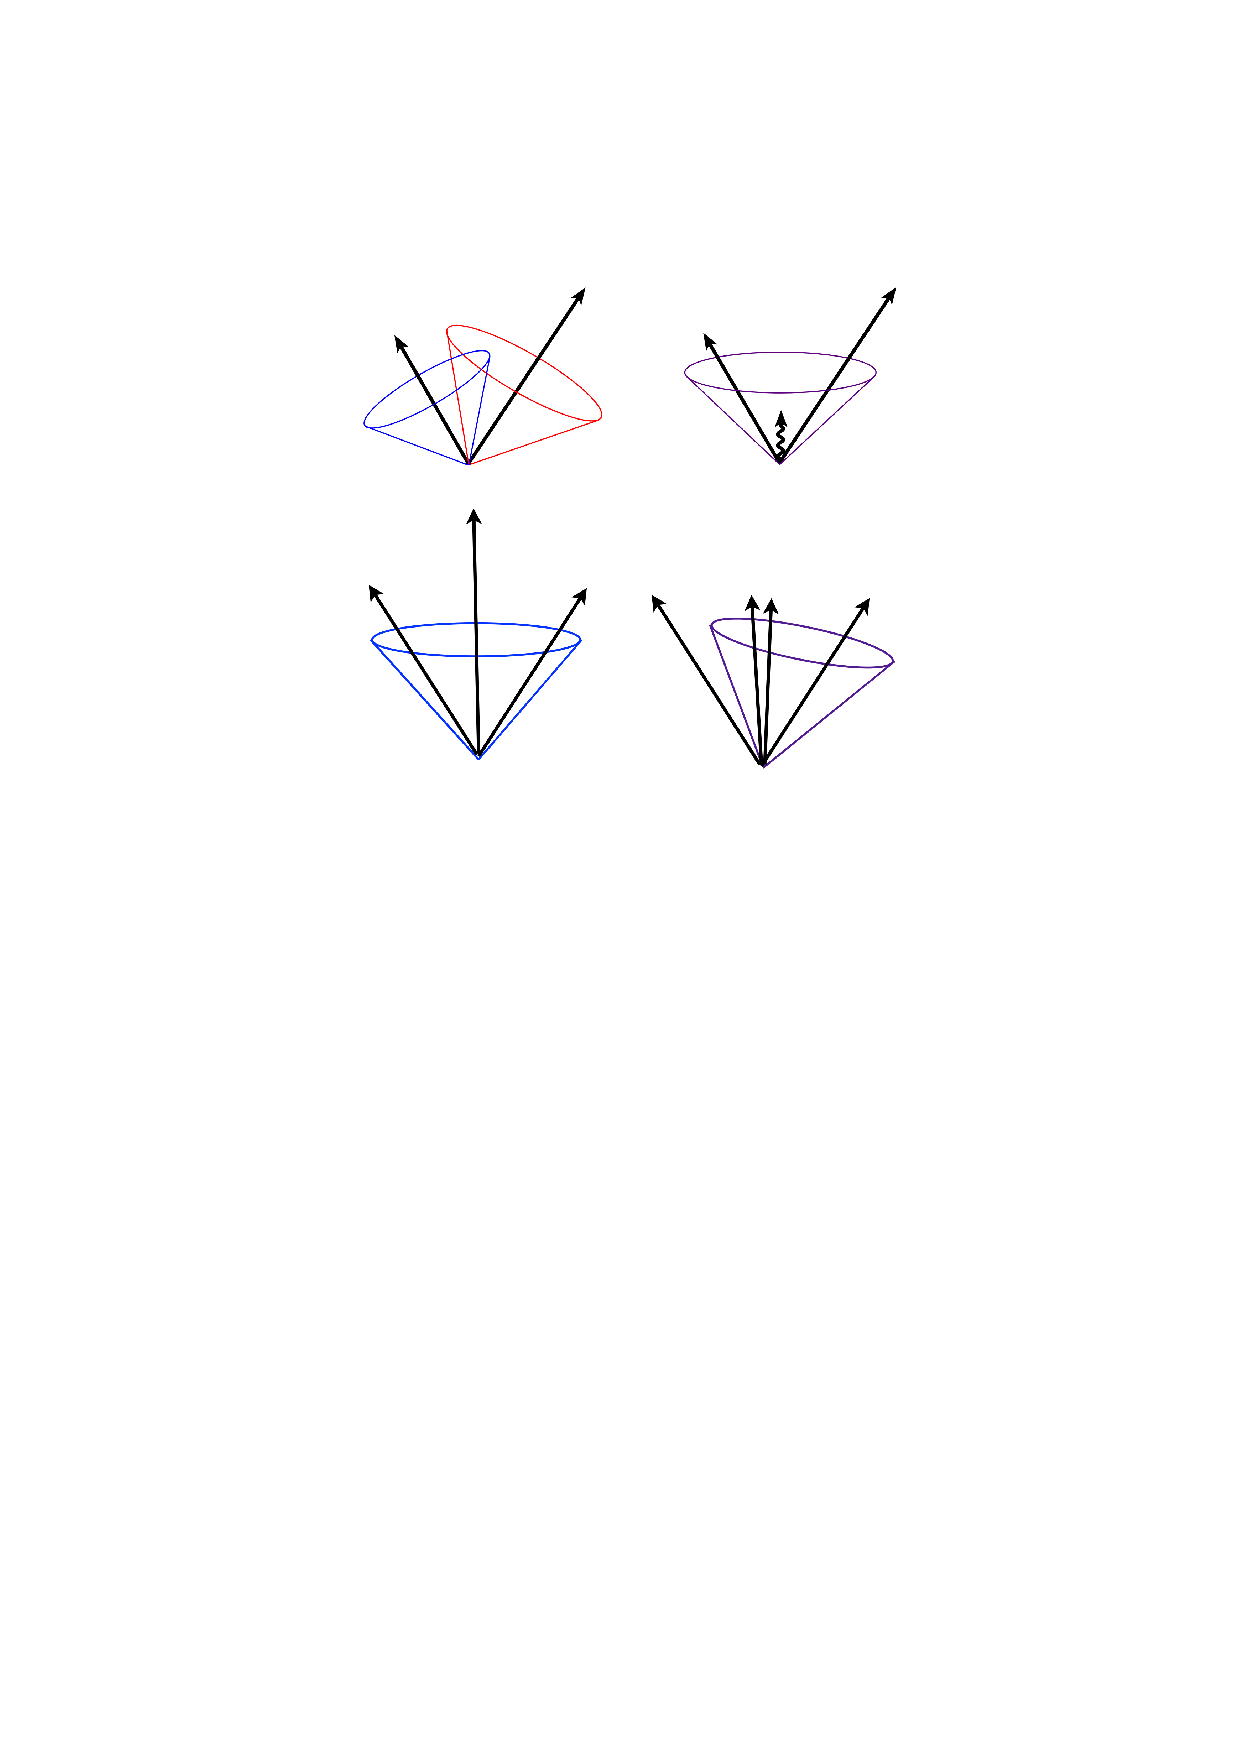
\includegraphics[scale = 0.9]{/home/anter/Desktop/Thesis/Figures/cropped_Algo.pdf}\\
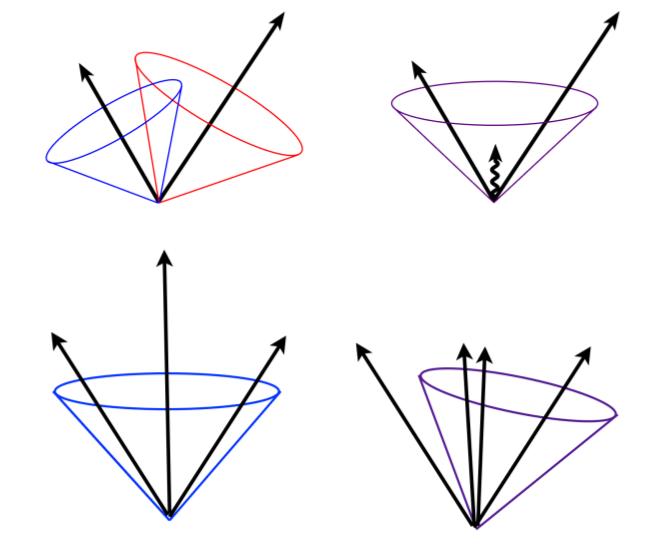
\includegraphics[scale = 0.55]{/home/anter/Desktop/Thesis/Figures/Final/Algo.png}\\
\caption[Illustration of infrared and collinear unsafe behaviour of jet algorithms.]{Top : Infrared unsafe behaviour of jet algorithm is illustrated where the presence of soft radiation between two jets may cause a merging of the jets that would not occur in the absence of the soft radiation. Bottom : Collinear unsafe behavior of jet algorithm is shown in which the number of jets change due to a collinear splitting\footnotemark.}
\label{fig:IRC}
\end{center}
\end{figure} \footnotetext{Source : \url{http://inspirehep.net/record/1251416}}This produces a single jet instead of initial two jets resulting in the change of number of jets. Collinear safety is the property by virtue of which the collinear splitting i.e. replacement of one parton by two at the same place should not modify the number of jets formed in an event. This implies that the output of the jet algorithm should remain the same if the energy of a particle is distributed among two collinear particles. According to the collinear safety property, the two cases shown in Fig.~\ref{fig:IRC} (bottom) should always produce a single jet. If an algorithm produces zero or two jets after collinear splitting, then it is not collinear safe. The jet algorithms can be classified mainly into two types : \\ \newline
{\bf Cone Algorithms -} In the iterative cone (IC) algorithm \cite{Blazey:2000qt}, the jet is defined as a cone with fixed radius $R$ in $\eta$-$\phi$ space drawn around the highest energy seed. The relative distance ($d$) of all the particles is iteratively calculated and compared with $R$. If the calculated $d$ \ls $R$, the considered particles are clustered together in a jet and the directions of the clustered particles give the direction of the jet. On the other side i.e. if $d$ \gr $R$, the considered particles initiate two different jets. The algorithm iterates until the cone is stable which means that the direction of sum of momentum of all the particles is same as that of the center of cone. But IC algorithm is not IRC safe. There is an another cone algorithm, Seedless Infrared-Safe cone (SIS-Cone) \cite{Weinzierl:2011jx}, which is an exact seedless i.e. does not rely on seed threshold and is IRC safe. This is a complex approach which tests the stability of all subsets of particles and has a complexity of ${\cal O}(N2^{N})$ for $N$ particles. But this algorithm is much slower and hence not preferred. \\ \newline
{\bf Sequential Recombination Algorithms -} The sequential recombination algorithms \cite{Ellis:1993tq} cluster the particles by defining a distance between pairs of particles and recombine the pair of closest particles successively. This is collinear and infrared safe algorithm. It is possible for cone jets to overlap such that one particle is contained in more than one jet but the sequential recombination algorithm never assigns a particle to more than one jet. The sequential recombination algorithm is based on transverse momentum \pt of the particles and follows the procedure as below : 
\begin{enumerate}
\item First the distance $d_{ij}$ between two particles $i$ and $j$ and distance $d_{iB}$ of the particle to the beam are calculated.\\
\begin{equation}
\begin{gathered}
d_{ij} = {\rm min}\big(p^{2p}_{{\rm T}i},p^{2p}_{{\rm T}j}\big) \frac{\Delta R^2_{ij}}{R^2}, ~~~~d_{iB} = p^{2p}_{{\rm T}i} \\ {\rm where} ~~~\Delta R^2_{ij} = (y_i -y_j)^{2} ~\plus (\phi_i -\phi_j)^{2}
\end{gathered}
\end{equation}

\item If $d_{ij}$ \ls $d_{iB}$, then the particles $i$ and $j$ are merged into a new single jet object $k$, summing four-momenta of two initial particles by recombination scheme and step 1 is repeated. 
\item If $d_{iB}$ \ls $d_{ij}$, particle $i$ is declared as a final-state jet and the particle gets removed from the list. 
\end{enumerate}
This procedure continues until all particles get clustered into jets. The value of the parameter $p$ defines the three different sequential algorithms having distinct properties. For $p$ = 1, we have \kt algorithm \cite{Catani:1993hr,Catani:1992zp}, $p$ = 0 gives the Cambridge/Aachen (C/A) algorithm \cite{Dokshitzer:1997in} whereas $p$ = -1 defines the anti-$k_{T}$ algorithm \cite{Cacciari:2008gp}. The \kt algorithm involves clustering of soft particles first resulting in an area that fluctuates considerably. This algorithm is susceptible to the underlying and pileup events. The C/A algorithm involves energy independent clusterings. Both \kt and C/A produce jets of irregular shapes. Instead of jet analysis, these are widely considered for studying the jet substructure. The anti-$k_{T}$ algorithm tends to cluster hard particles first and produces jets with more regular circular shapes. It is less sensitive to underlying and pileup events. It is the most preferred algorithm for jet studies at the LHC. Figure~\ref{fig:jet_algo} shows the clustering of same particles but using the different jet algorithms. 

\begin{figure}[!h]
\begin{center}
\hspace*{-10mm}
%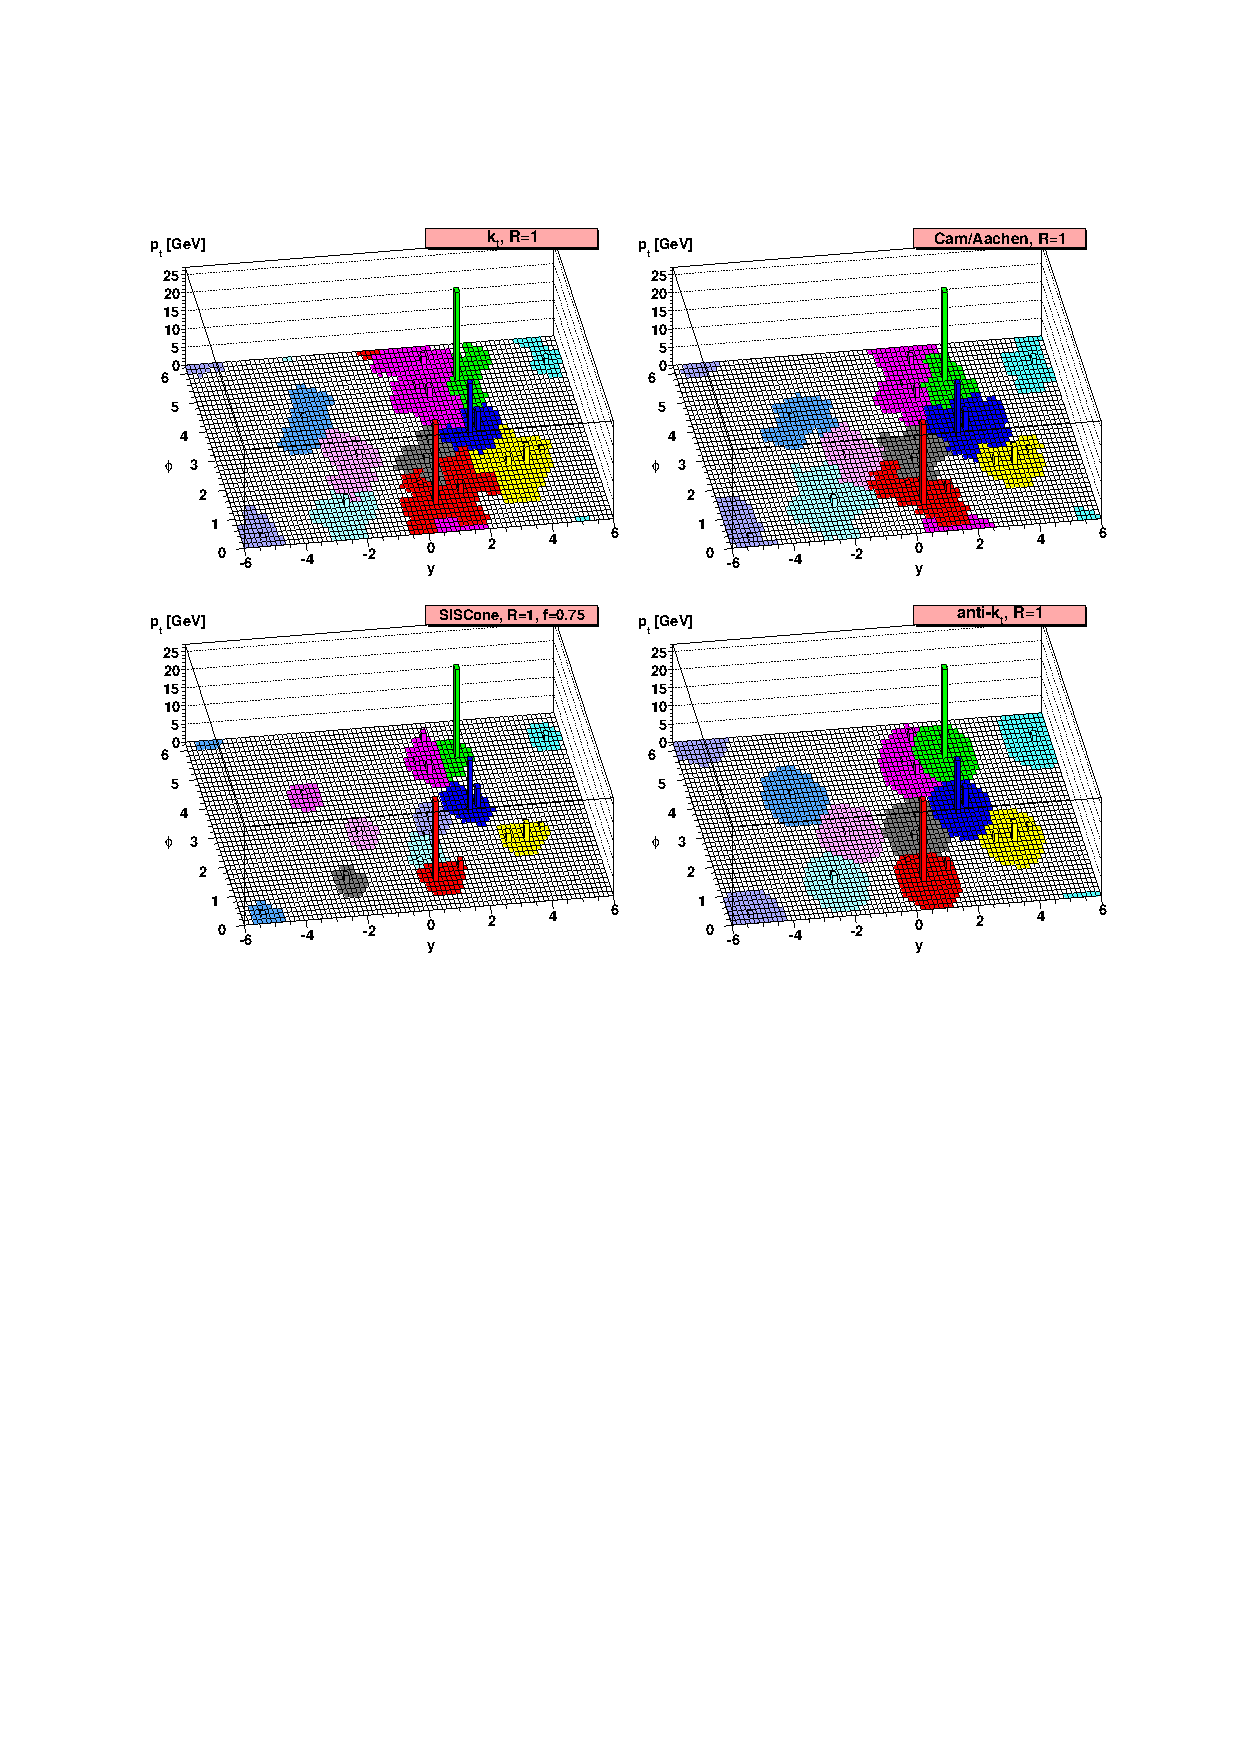
\includegraphics[width=1.2\textwidth]{/home/anter/Desktop/Thesis/Figures/cropped_JetAlgo.pdf}\\
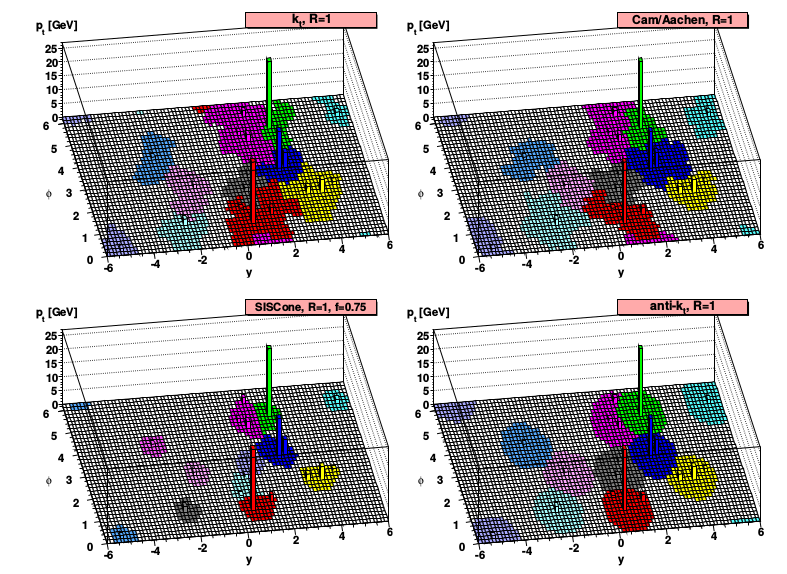
\includegraphics[width=1.1\textwidth]{/home/anter/Desktop/Thesis/Figures/Final/JetAlgo.png}\\
\vspace*{4mm}
\caption[The clustering of particles into jets using different jet algorithms.]{The clustering of particles, in $y$-$\phi$ space at the parton level, into jets clustered with the \kt (top left), Cambridge/Aachen (top right), SISCone (bottom left) and anti-\kt (bottom right) algorithms with $R$ = 1. The towers represent the jet \pt. The anti-\kt algorithm gives circular jets while the jets produced with other three algorithms have irregular shapes. Taken from \cite{Salam:2009jx}.}
\label{fig:jet_algo}
\end{center}
\end{figure}

A jet algorithm must specify how to combine the momenta of different partons or particles going to be clustered into a jet. This is given by the recombination scheme. The most widely used recombination scheme is the $E$-scheme \cite{Blazey:2000qt} which corresponds to vector addition of four-momenta where the four-momenta of the jet is obtained by simply adding the four-momenta vectors of merging particles.
 
The sequential clustering algorithms have traditionally been favoured by theorists but not by experimentalists because of slow computational performance. However, the introduction of the \fastjet program \cite{Cacciari:2011ma} enhanced the speed of clustering algorithms and hence are preferred by experimentalists as well. This thesis details the particles produced in proton-proton collisions by clustering them in to jets using anti-\kt algorithm with distance parameter $R$ = 0.7. These jets are observed in the Compact Muon Solenoid detector of the Large Hadron Collider, the details of which are discussed in the following chapter.

  %Chapter 2
%%\chapter{Experimental Setup}
\label{chap:Detector}
%\cite{Evans:2008zzb} \cite{LEP}
The hadron colliders aim at search for elementary particles and their interactions as predicted in the Standard Model or theories beyond the Standard Model. For the same beam energy, higher center-of-mass energy can be achieved by the hadron colliders as compared to fixed target experiments. Due to the availability of very high center-of-mass energy for the collisions, it becomes possible for the researchers to understand the fundamental structure of the universe deeply and to look back in its history. The precise measurement of mass of the $Z$ and $W$ boson discovered by the UA1 and UA2 experiments was done at the Large Electron-Positron (LEP) collider. The discovery of top quark and an acute measurement of its mass was performed by the proton-antiproton collider Tevatron at FNAL. The search for the long awaited Higgs boson was carried out by the currently running most powerful accelerator, the Large Hadron Collider (LHC). Still many questions related to the the nature of dark matter, the existence of super-symmetry (SUSY) or the extra dimensions are yet to be answered. 

The European Organization for Nuclear Research (CERN) is a world-class fundamental physics research organization founded in 1954. In the beginning, it concentrated on pure physics research to understand the inside of the atom, justifying the word ``nuclear'' in name. At present, the main area of research at CERN is particle physics - the study of the fundamental constituents of matter and the forces of interactions acting between them. To complete this task, several particle accelerators have been built by CERN to explore the physics at the TeV energy scale.

\section{The Large Hadron Collider}
The Large Hadron Collider (LHC) \cite{Evans:2008zzb} is the world's biggest and the most powerful particle accelerator and collider built by CERN. It occupies the 27 km circumference circular tunnel (between the border of France and Switzerland), previously used by LEP collider \cite{LEP}, at a depth ranging from 50 to 175 metres (164 to 574 ft) underground. Two beams of particles of the same kind, either protons or lead or xenon ions, are accelerated in direction opposite to each other. 1,232 dipole magnets maintain the beams in their circular path and 392 quadrupole magnets keep the beams focused to increase the probabilities of interaction between the particles. Since this thesis is based on the proton-proton (pp) collisions data, the main focus is on protons. 

The protons pass through a series of accelerators which increase their energy successively before their injection into the main ring of LHC. Figure~\ref{fig:LHC} gives an overview of the various accelerators and detectors comprising the complex structure of the LHC. The protons are obtained by stripping of electrons from hydrogen gas atoms using an electric field. The protons are accelerated up to 100 keV through a radiofrequency quadrupole which provides the first focusing and a further acceleration to 750 keV energy. The linear particle accelerator (LINAC2) increases the energy of protons to 50 MeV. Then these protons are injected into the Proton Synchrotron Booster (PSB) in the form of bunches where they get accelerated to 1.4 GeV energy. The energy of protons is further enhanced to 25 GeV by Proton Synchrotron (PS) and then to 450 GeV by the Super Proton Synchrotron (SPS). Finally the protons are injected into two beam pipelines of the main LHC ring where their energy increases to the collision energy. In head on collisions for colliding beams of the same mass particles, the center of mass system and the laboratory system coincide and the total center of mass energy is twice the energy of the beams. 

\begin{figure}[!h]
 \begin{center} 
 \hspace*{-5mm}
 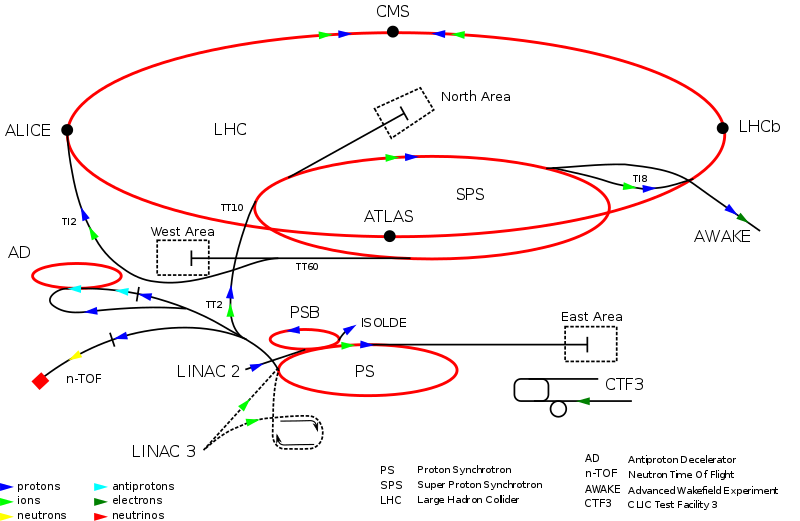
\includegraphics[width=1.\textwidth]{/home/anter/Desktop/Thesis/Figures/LHC.png}\\
 \vspace*{5mm}
 \caption[Overview of the different experiments of the Large Hadron Collider (LHC), a complex particle accelerator and collider located at CERN.]{Overview of the different experiments of the Large Hadron Collider (LHC), a complex particle accelerator and collider located at CERN\footnotemark.}
 \label{fig:LHC}
 \end{center}
\end{figure}
\footnotetext{Source : \url{https://en.wikipedia.org/wiki/Large_Hadron_Collider}}

The accelerated beams are made to collide at four interaction points around which six detectors : ALICE (A Large Ion Collider Experiment) \cite{Aamodt:2008zz}, ATLAS (A Toroidal LHC Apparatus) \cite{Aad:2008zzm}, CMS (Compact Muon Solenoid) \cite{Chatrchyan:2008aa,Bayatian:2006nff,Ball:2007zza}, LHCb (Large Hadron Collider for Beauty) \cite{Alves:2008zz}, LHCf (Large Hadron Collider forward)\cite{Adriani:2008zz} and TOTEM (Total, elastic and diffractive cross-section measurement) \cite{Anelli:2008zza}, are located. The CMS and ATLAS are the two general purpose detectors dedicated to the search of the Higgs boson, existence of super-symmetry (SUSY) and also looking for extra dimensions. The ALICE is a heavy-ion detector which collides lead ions to study quark-gluon plasma, a state of matter believed to be present just after the Big Bang. The LHCb experiment will explore the differences between matter and antimatter and new physics through b-quark (beauty) studies. TOTEM experiment is dedicated to cross-section measurements whereas LHCf focuses on forward physics. 

The LHC successfully injected the first protons on September 10, 2008 but after few days magnetic quench occurred in about 100 bending magnets leading to a loss of $\sim$6 tonnes of liquid helium. The low-energy beams circulated in the tunnel for the first time on November 20, 2009 and after three days, the first particle collisions took place in all four detectors at \cme = 450 GeV. The LHC achieved 1.18 TeV energy per beam on November 30, 2009 and become the world’s highest energy particle accelerator leaving behind the Tevatron with record of 0.98 TeV per beam for eight years. The pp collisions at \cme = 2.36 TeV were recorded around December 15, 2009. On March 19, 2010, the beam energy was ramped up to 3.5 TeV, resulting in the first pp collisions at \cme = 7 TeV on March 30, 2010. The beam energy was kept at 3.5 TeV throughout 2011, and increased to 4 TeV in 2012. After a long shutdown for two years, the LHC restarted in 2015 and collided the proton beams at a much higher centre-of-mass energy of 13 TeV and is running successfully till now. In the coming years, protons will be made to collide at a designed \cme = 14 TeV with luminosity up to 10$^{34}$ cm$^{-2}$s$^{-1}$. In this thesis, work has been carried out using the pp collisions data collected by the CMS detector at \cme = 8 TeV in the year of 2012.

\subsection{Luminosity Measurement}
\label{sec:lumi}
Luminosity (\lumi) is one of the most important parameters of an accelerator which characterizes its performance. It gives the rate at which collisions occur and given by the number of collisions produced in a detector per cm$^2$ and per second. Cross-section ($\sigma$) is a measurement of the probability that an event will occur. It is related to total number of events $N$ of a process over a time period T and \lumi as :
\begin{equation}
N = \int_{0}^{T} \lumi~\sigma~dt = \lumi_{int}~\sigma
\end{equation}
where $\int_{0}^{T} \lumi~dt = \lumi_{int}$ is the total integrated luminosity. It is expressed in units of area, usually in barn$^{-1}$ and gives a direct indication of the number of produced events for a process. For example, an integrated luminosity of 10 fb$^{-1}$ means that 10 events are produced in a process with cross-section equal to 1 fb.

The luminosity depends on the particle beam parameters and is given by :

\begin{equation}
\lumi = \frac{N^2_p~N_b~f_{rev}~\gamma~F}{4\pi~\epsilon_n~\beta^*}
\end{equation}
where $N_p$ is the number of particles per bunch, $N_b$ is the number of bunches per beam, $f_{rev}$ is the revolution frequency of the beam, $\gamma$ is the relativistic gamma factor and $F$ gives the geometric luminosity reduction factor. The effective collision area of the two beams is related to the normalized transverse beam emittance $\epsilon_n$ and the value of the betatron function $ \beta^*$ at the interaction point.
 
The CMS experiment constantly monitors the instantaneous luminosity delivered by LHC which is shown versus time in Fig.~\ref{fig:lumi} for proton-proton collisions at nominal center-of-mass energy for the years 2010-2017. The relative instantaneous luminosity is calculated by using two methods \cite{CMS:2013gfa} : Hadron Forward (HF) method by measuring the particle flux in the hadron forward calorimeter and by counting the number of reconstructed vertices in the pixel tracker. The absolute luminosity measurement relies on van-der-Meer scans done in special runs of the LHC \cite{vanderMeer:1968zz}. The uncertainty on the luminosity measured for 2012 data set is 2.5\% (syst.) and 0.5\% (stat.).

\begin{figure}[!h]
 \begin{center}
 \vspace*{4mm} 
 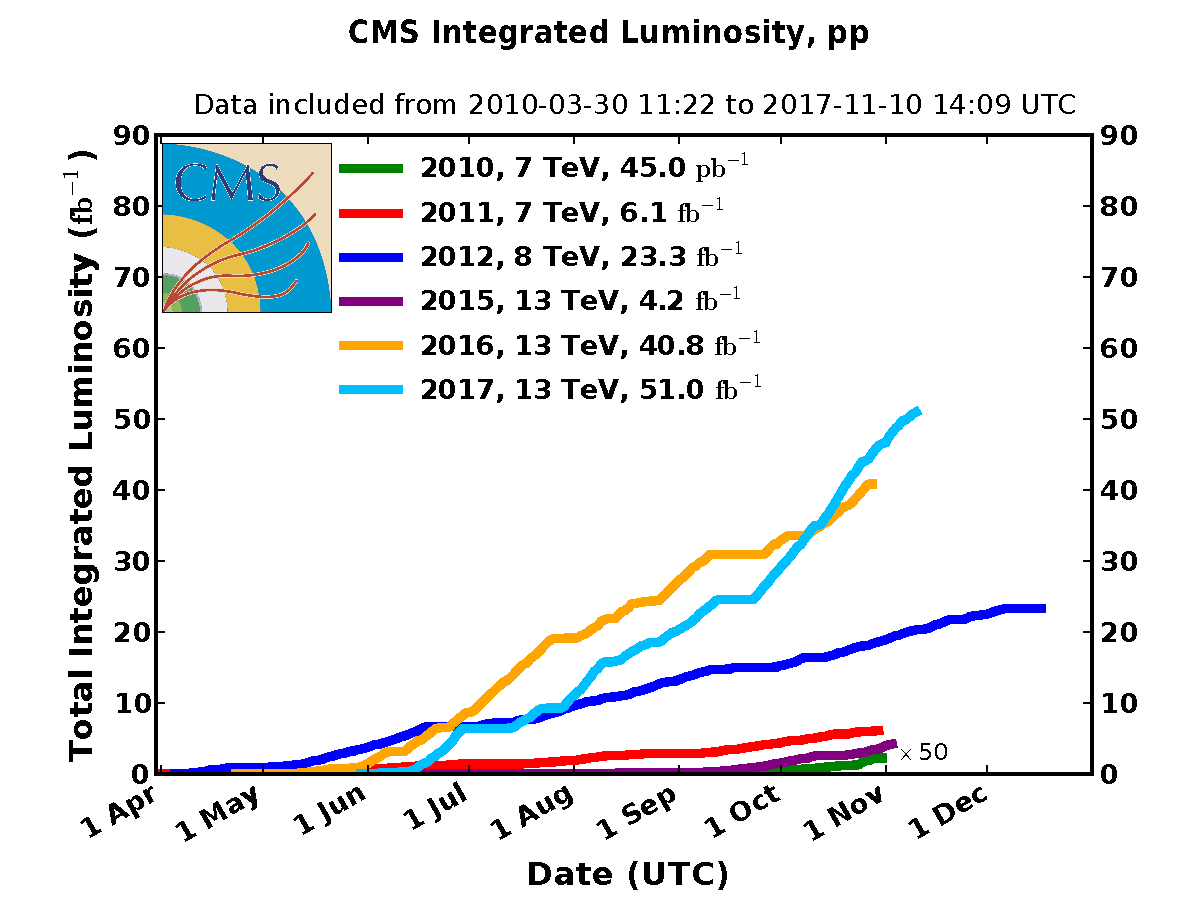
\includegraphics[width=.8\textwidth]{/home/anter/Desktop/Thesis/Figures/int_lumi_cumulative_pp_2.pdf}\\
 \vspace*{5mm}
 \caption[The integrated luminosity, delivered to CMS during stable beams for proton-proton collisions.]{The integrated luminosity, delivered to CMS during stable beams for proton-proton collisions at nominal center-of-mass energy, is shown versus time for data-taking in 2010 (green), 2011 (red), 2012 (blue), 2015 (purple), 2016 (orange) and 2017 (light blue) run periods of the LHC\footnotemark.}
 \label{fig:lumi}
 \end{center}
\end{figure}
\footnotetext{Source : \url{https://twiki.cern.ch/twiki/bin/view/CMSPublic/LumiPublicResults}}

\subsection{Pileup Interactions}
To observe the extremely rare events, the event rate in a collider should be very high. This demands delivered luminosity to be high which is achieved by increasing the number of bunches or increasing the number of protons per bunch. However, this comes at the cost of multiple proton-proton interactions coming from independent hadron-hadron collisions occurring in the same bunch crossing, called pileup (PU) interactions. The hard interaction in every event is accompanied by a large amount of PU interactions which give rise to low \pt jets. The vertex of pile-up interaction is reconstructed from tracks pointing to it as shown in Fig.~\ref{fig:pileup_d}. The pileup due to additional collisions within a single bunch crossing is called in-time pileup whereas pileup coming from collisions other than hard scattering in other bunch crossings is known as out-of-time pileup. The pileup itself cannot be directly measured, it can be correlated to various other directly measurable quantities. Since pileup comes from additional proton-proton interactions, the number of primary vertices ($N_{PV}$) is directly correlated to the amount of pileup. The greater the $N_{PV}$, the more pileup energy is added to the jets which needs to be subtracted. 
\begin{figure}[!h]
 \begin{center}
 \vspace*{4mm} 
 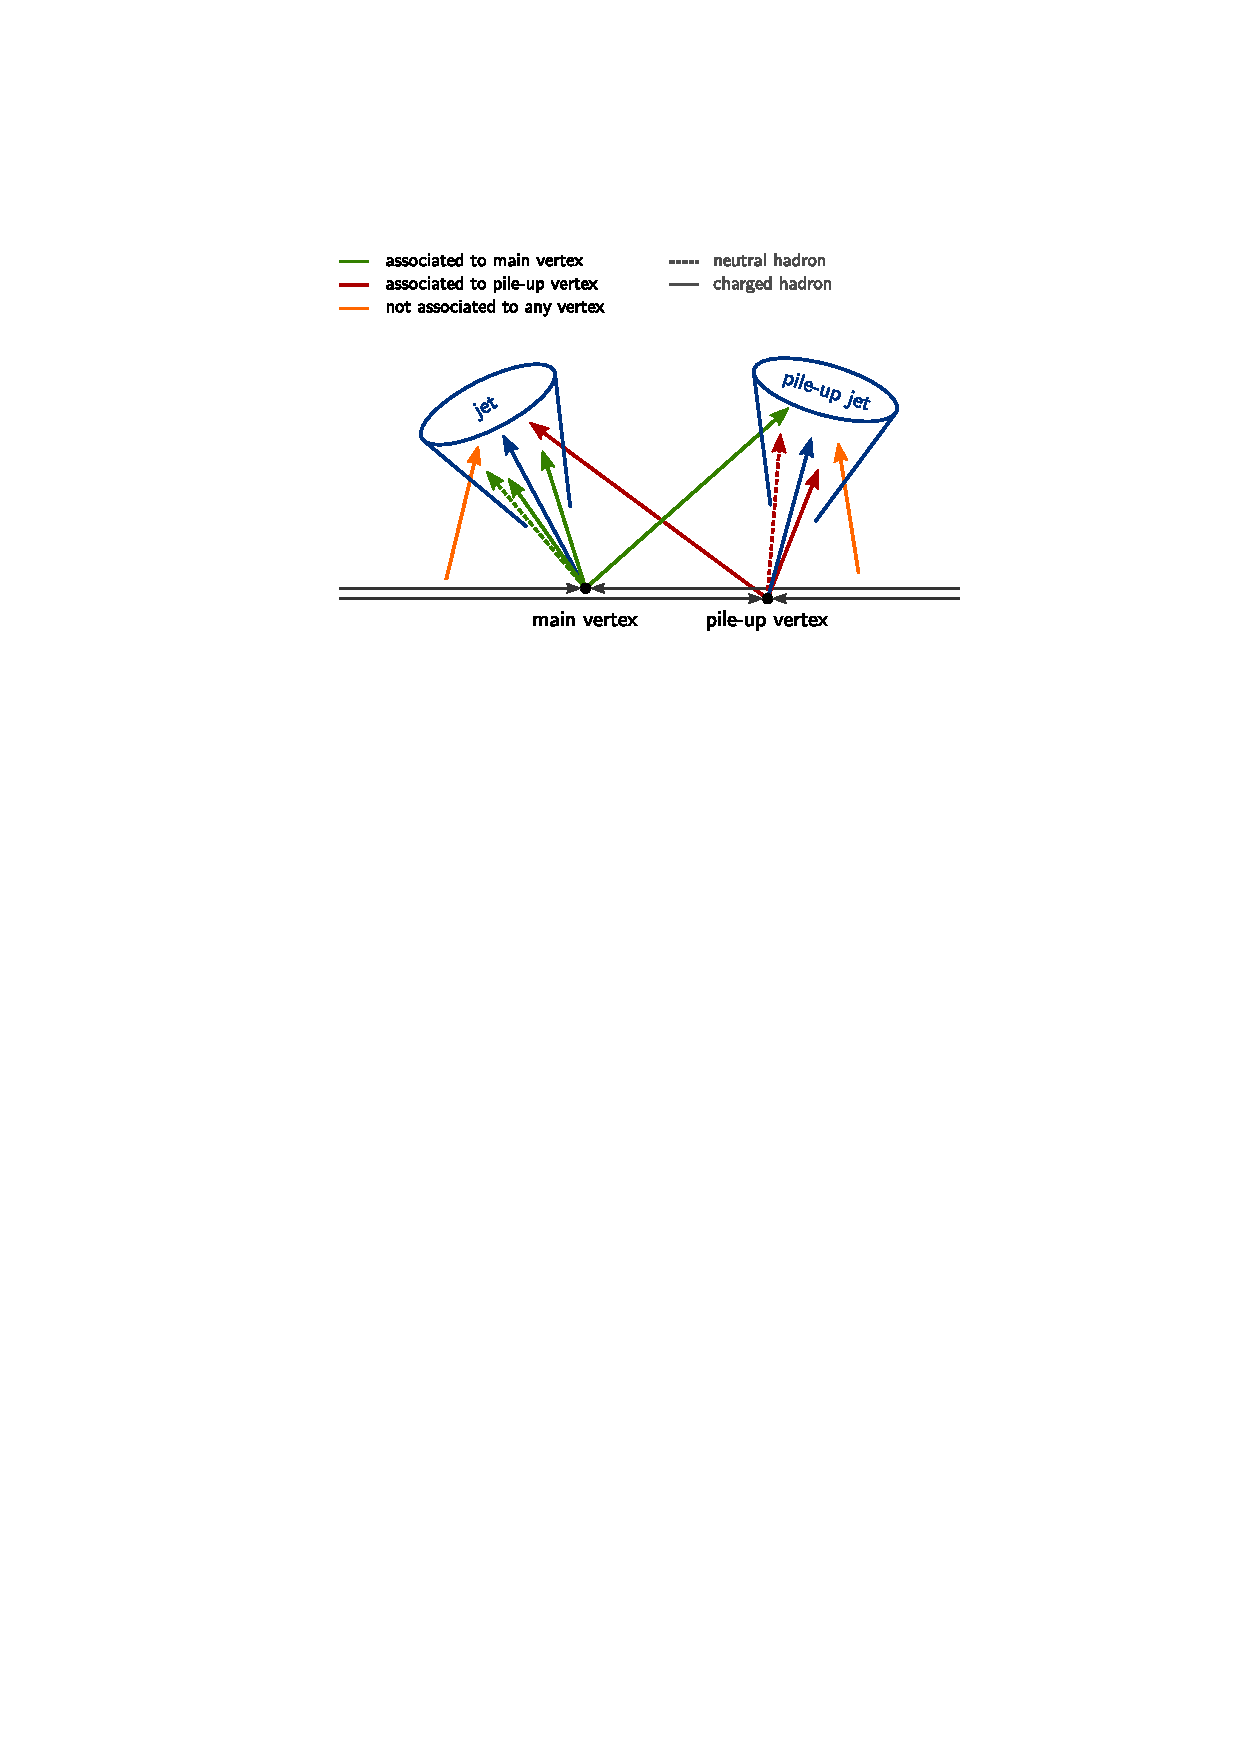
\includegraphics[width=.8\textwidth]{/home/anter/Desktop/Thesis/Figures/cropped_Pileup.pdf}\\
 \vspace*{5mm}
 \caption[Pileup Interactions]{In a proton-proton collision, the particles produced from the hard interaction are clustered into a jet. The hard interaction corresponds to the main vertex. The particles produced in the interactions other than the hard one, form a pileup jet\footnotemark.}
 \label{fig:pileup_d}
 \end{center}
\end{figure}
\footnotetext{Source : \url{http://cds.cern.ch/record/1747055}}

\section{The Compact Muon Solenoid}
The Compact Muon Solenoid (CMS) detector is a general purpose detector located at the interaction point 5 (P5) of the main LHC ring, near the village of Cessy in France. The name of CMS comes from its compact size with main emphasis on the detection of muons and enclosed within high solenoidal magnetic field. The CMS detector aims at identifying the different types of particles produced in proton-proton and heavy ion collisions and measuring their energies and momenta. This is achieved by concentric layers of different sub-detectors arranged in a cylindrical complex structure with 21.6 m length and 15 m diameter. The silicon-based tracker surrounds the the interaction point and forms the innermost layer. It is surrounded by a scintillating crystal electromagnetic calorimeter (ECAL) and a sampling hadron calorimeter (HCAL) which are enclosed inside the superconducting solenoid. Outside the magnet lies the large muon detectors embedded inside an iron yoke. 
\begin{figure}[!h]
\begin{center}
\vspace{2mm}
\hspace*{-6mm}
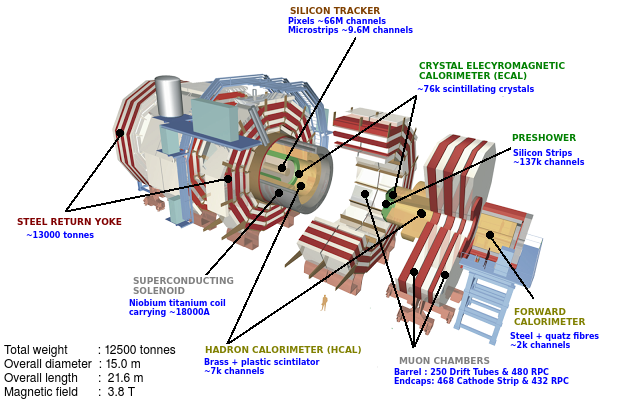
\includegraphics[scale = 0.98]{/home/anter/Desktop/Thesis/Figures/CMS_2_new.png}\\
\vspace*{5mm}
\caption[The three dimensional view of the CMS detector along with its sub-detector components.]{The three dimensional view of the CMS detector along with its sub-detector components\footnotemark.}
\label{fig:CMS}
\end{center}
\end{figure}
\footnotetext{Source : \url{https://orbiterchspacenews.blogspot.in/2013/04/cern-cms-prepares-for-future.html}}
The three dimensional view of the CMS detector along with its components is presented in Fig.~\ref{fig:CMS}. The CMS was constructed in parts at ground and assembled later on in the cavern. The components are easily accessible for upgrades or repairs as the detector can be opened up into movable slices. Figure~\ref{fig:CMS_front} shows the front view of the CMS detector differentiating individual components which contribute to event reconstruction. The path of reconstructed particles is represented by dashed (invisible track) and solid (visible track) lines for different particle classes : photons ($\gamma$), muons ($\mu^{\pm}$), electrons (e$^{-}$), neutrons (n) and charged hadrons (pions $\pi^{\pm}$).

\begin{figure}[!h]
\begin{center} 
\hspace*{-15mm}
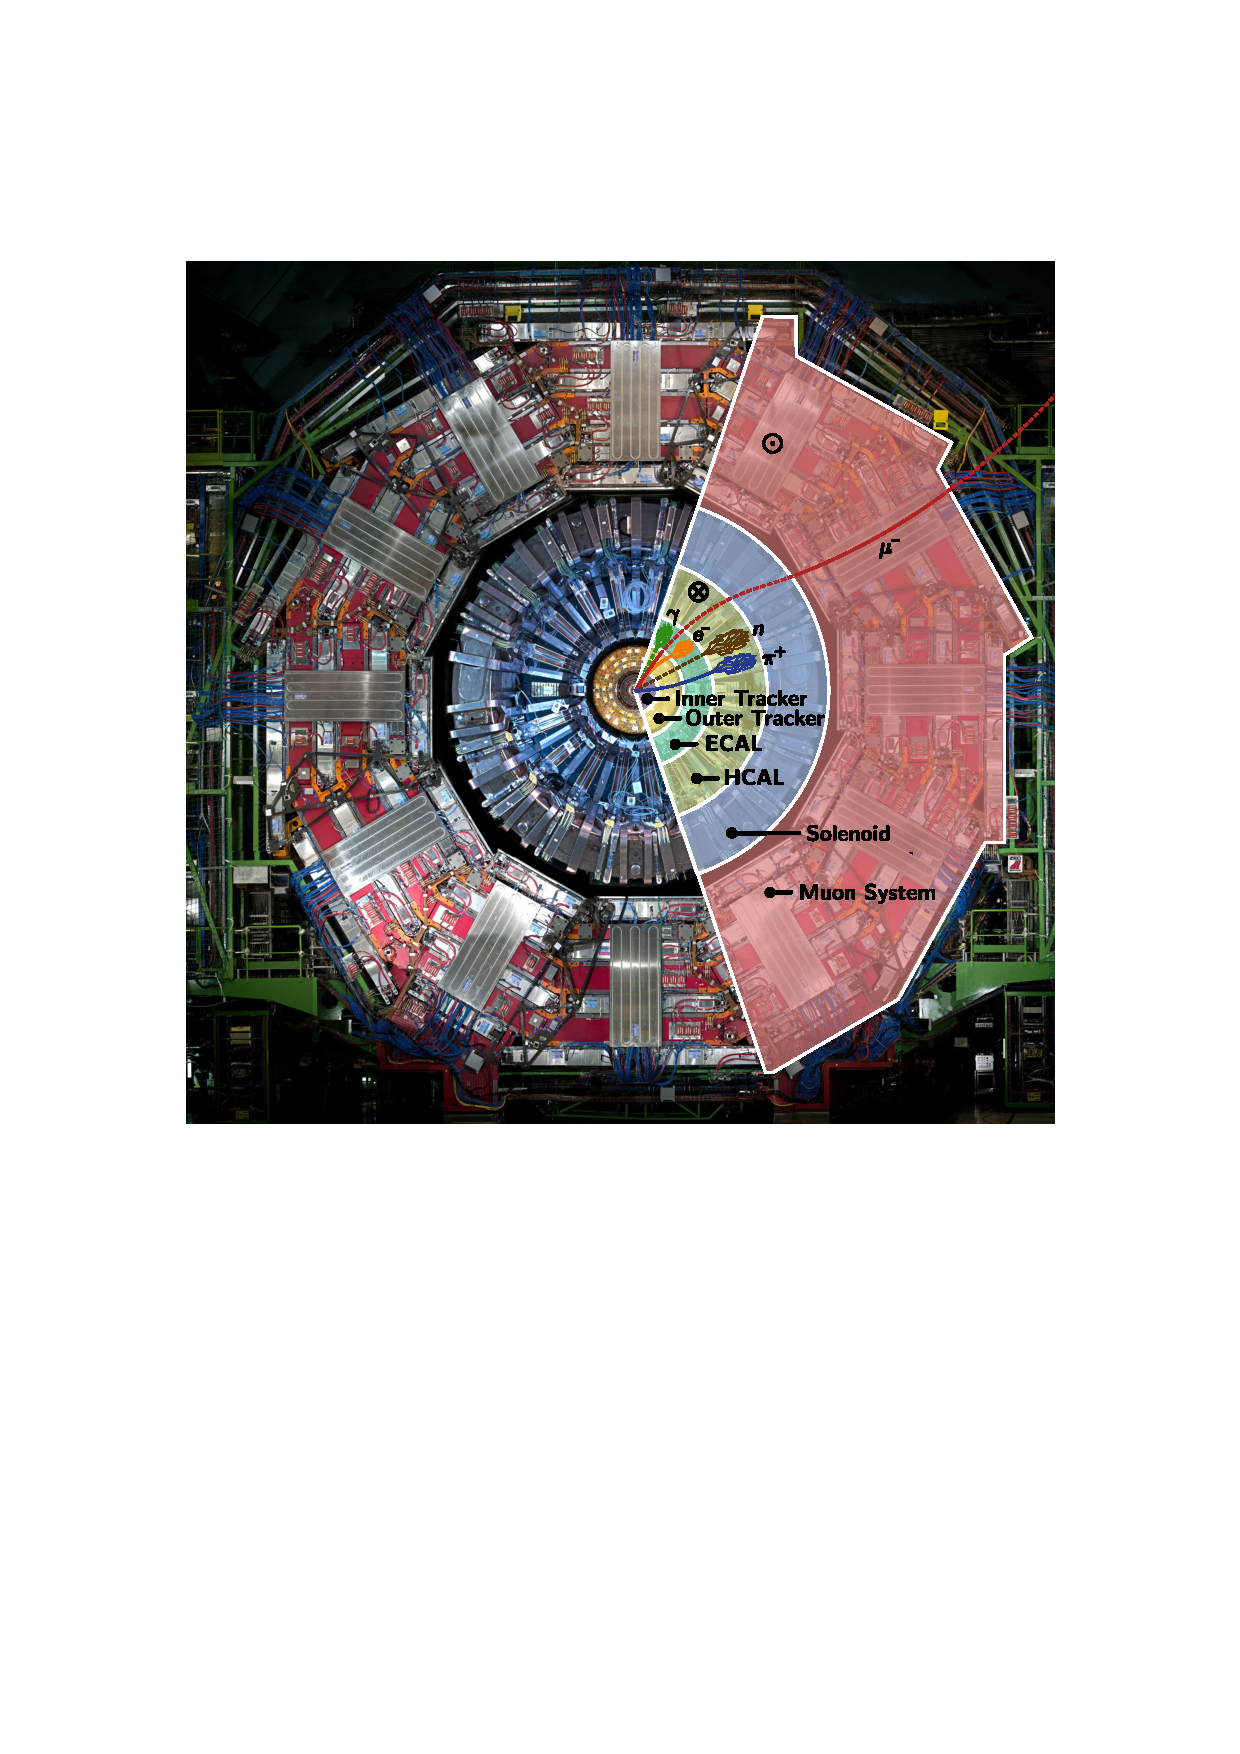
\includegraphics[scale = 0.55]{/home/anter/Desktop/Thesis/Figures/cropped_CMS_Front.pdf}
\caption[Front view of the CMS detector along with its components.]{Front view of the CMS detector along with its components : inner tracker, outer tracker, electromagnetic calorimeter, hadronic calorimeter, solenoid and muon system. The path of different particles detected by dedicated sub-detectors are shown by dashed (invisible track) and solid (visible track) lines. $\otimes$ and $\odot$ gives the direction of magnetic field inside the solenoid and in the return yoke, respectively. Taken from \cite{Ball:2007zza}.}
\label{fig:CMS_front}
\end{center}
\end{figure}

A brief overview of the CMS detector has been presented and the details of the its design as well as physics performance are available in Ref.~\cite{Bayatian:2006nff,Ball:2007zza}. Before going into the details of each sub-detector, first the CMS coordinate system is described in the next section.

\subsection{Coordinate System}
CMS uses right-handed coordinate system, illustrated in Fig.~\ref{fig:coordinate}, having origin at the nominal interaction point (IP) of the collision inside the detector. The $x$-axis points horizontally from the IP, towards the center of the LHC ring, the $y$-axis vertically upwards and the $z$-axis along the beam direction towards the Jura mountains. The radial coordinate in $x$-$y$ plane is denoted by $r$. 
\begin{figure}[!h]
\begin{center} 
\hspace*{-15mm}
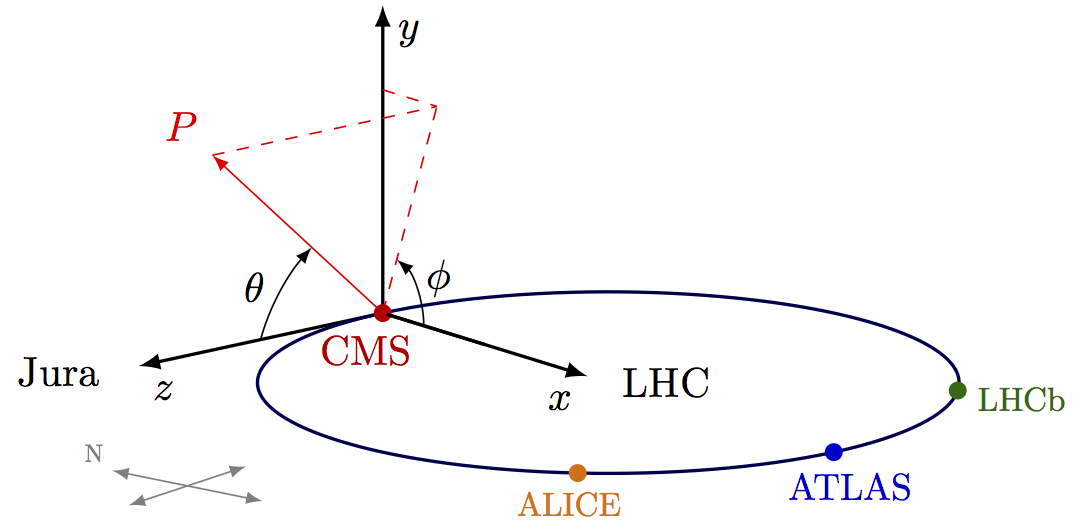
\includegraphics[scale = 1.5]{/home/anter/Desktop/Thesis/Figures/cms_coordinate_system.png}
\vspace{3mm}
\caption[The right-handed coordinate system used by the CMS detector.]{The right-handed coordinate system used by the CMS detector\footnotemark with origin at the interaction point (IP), $x$-axis points horizontally from the IP towards the center of the LHC ring, the $y$-axis vertically upwards and the $z$-axis along the beam direction towards the Jura mountains, $\phi$ as the azimuthal angle measured from the $x$-axis in the $x$-$y$ plane and $\theta$ as the polar angle calculated from the $z$-axis in the $z$-$y$ plane.}
\label{fig:coordinate}
\end{center}
\end{figure}
\footnotetext{Source : \url{https://wiki.physik.uzh.ch/cms/latex:example_spherical_coordinates}}
Following customary polar coordinate conventions : the azimuthal angle $\phi$ is measured from the $x$-axis in the $x$-$y$ plane as $\phi = {\rm tan^{-1}}(\frac{y}{x})$ where $\phi$ = 0 points to the \plusn $x$ axis and $\phi$ = $\pi$/2 points to the \plusn $y$ axis. The polar angle $\theta$, is calculated from the $z$-axis in the $z$-$y$ plane as $\theta~=~{\rm tan^{-1}}\big(\frac{x^2~\plus y^2}{2}\big)$ with $\theta$ = 0 corresponding to the \plusn $z$ direction and $\theta$ = $\pi$ to the -$z$ direction. The quantities pseudorapidity $\eta$ and the rapidity $y$ are preferred over the angles $\theta$ and $\phi$. The pseudorapidity and rapidity are given by Eq.~\ref{eq:pseudorap}. Both the quantities are equal for massless particles.
\begin{equation}
\begin{gathered}
\eta = -~{\rm ln}\bigg({\rm tan}\bigg(\frac{\theta}{2}\bigg)\bigg)\\
y = \frac{1}{2}~{\rm ln} \bigg(\frac{E~\plus p_z}{E - p_z} \bigg)
\end{gathered}
\label{eq:pseudorap}
\end{equation}
The difference between rapidities $\Delta y$ is invariant under longitudinal Lorentz boost whereas it does not hold for $\eta$. Hence $y$ is considered in this thesis. The angular distance between the two particles is defined by $\Delta R = \sqrt{(\Delta \eta)^2~\plus (\Delta \phi)^2}$. The momentum component transverse to the direction of beam \pt, is computed from the $x$- and $y$-components as \pt = $\sqrt{p^2_x~\plus p^2_y}$ and the transverse energy is given by $E_T$ = $E$ sin$\theta$. After introducing the CMS coordinate system, further the detector subsystems are described briefly in the following sections. A longitudinal section of the CMS detector in the $y$-$z$ plane, shown in Fig.~\ref{fig:CMS_quad}, locates the different sub-systems along with the superconducting solenoid.

\begin{figure}[!h]
\vspace*{2mm}
\begin{center} 
\hspace*{-5mm}
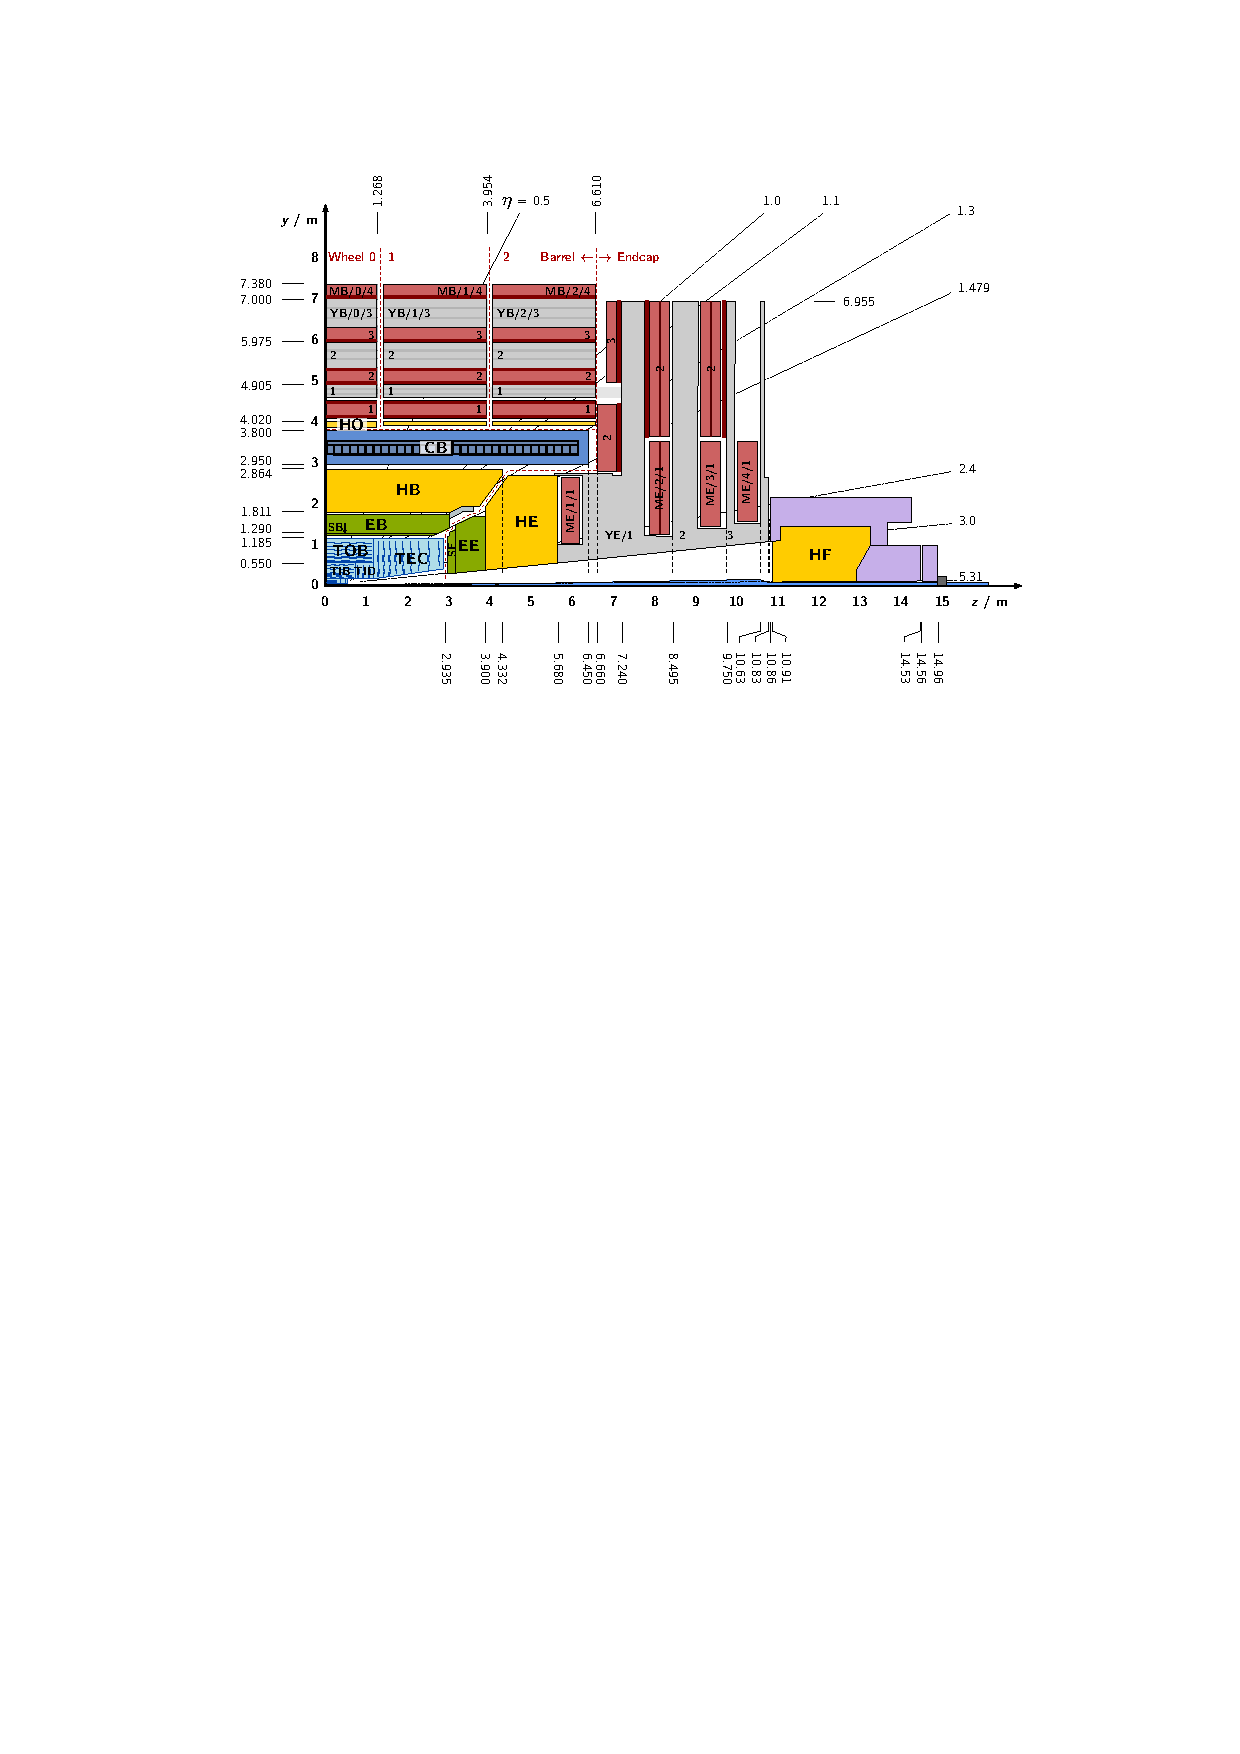
\includegraphics[scale = 1.1]{/home/anter/Desktop/Thesis/Figures/cropped_CMS_Quad.pdf}
\vspace{3mm}
\caption[Longitudinal section of the CMS detector in the $y$-$z$ plane.]{Longitudinal section of the CMS detector in the $y$-$z$ plane\footnotemark. It shows the tracking detector (TIB, TID, TOB, TEC) close to the nominal interaction point at (0,0), the electromagnetic (EB, EE) and hadronic (HB, HE, HO, HF) calorimeters. The coil of the solenoid magnet (CB) surrounds the inner barrel region. The iron return yoke (YB, YE) is interleaved with the muon chambers (MB, ME).}
\label{fig:CMS_quad}
\end{center}
\end{figure}

\subsection{Inner Tracker System}
The charged particles produced from the LHC collisions leave their trajectories as they move outward from the interaction point. The particle flux within the detector decreases as 1/$r^2$. So the tracks of the particles need to be measured as close to the collision point as possible and in a precise manner. The innermost tracking system of the CMS consisting of silicon detectors measures the hits of charged particles. It surrounds the interaction point and has a cylindrical volume of length of 5.8 m and a diameter of 2.5 m and covers a pseudorapidity range up to $|\eta|$ \ls 2.5. When charged particles pass through the silicon detector material, small ionization currents are produced which are detected as a hit. Such multiple hits when combined, reconstruct the track which gives the information about the direction and transverse momentum \pt of the charged particle. Silicon detectors have a much higher resolution in tracking charged particles as compared to the older ones such as cloud chambers or wire chambers.\footnotetext{Source : \url{http://cds.cern.ch/record/1747055}} CMS inner tracking system shown in Fig.~\ref{fig:tracker} consists of two sub-systems :\\ \newline 
{\bf Pixel Detector -} A pixel detector lying close to the beam pipe have three co-centric barrel layers at radii of 4.4, 7.3 and 10.2 cm from the beam pipe. It has two disks of pixel modules on each side of barrel. At the LHC design luminosity of 10$^{34}$ cm$^{-2}$s$^{-1}$, about 1000 particles from more than 20 overlapping proton-proton interactions traverse through the tracker for each bunch crossing, i.e. every 25 ns. The size of each pixel is 100 $\micro$m $\times$ 150 $\micro$m which gives an average occupancy of 10$^{-4}$ per bunch crossing. By taking an advantage of the large Lorentz effect, the pixel tracker has a resolution of 10 $\micro$m $\times$ 20 $\micro$m needed for a precise determination of the primary and secondary vertices and the required momentum resolution. \\ \newline
{\bf Strip Detector -} After coming out of the pixel detector the charged particles pass through ten layers of silicon strip detectors, reaching out to a radius of 130 cm. The silicon strip detector consists of four inner barrel (TIB) layers assembled in shells with two inner endcaps (TID), each composed of three small discs. The outer barrel (TOB) consists of six concentric layers. Finally two endcaps (TEC) close off the tracker. Each part has silicon modules designed differently for its place within the detector. The strip detector measures the particle tracks with a reduced resolution of 23 $\micro$m reflecting the smaller particle flux at larger distances from the interaction point.
\begin{figure}[!h]
\begin{center} 
\vspace*{2mm}
\hspace*{-6mm}
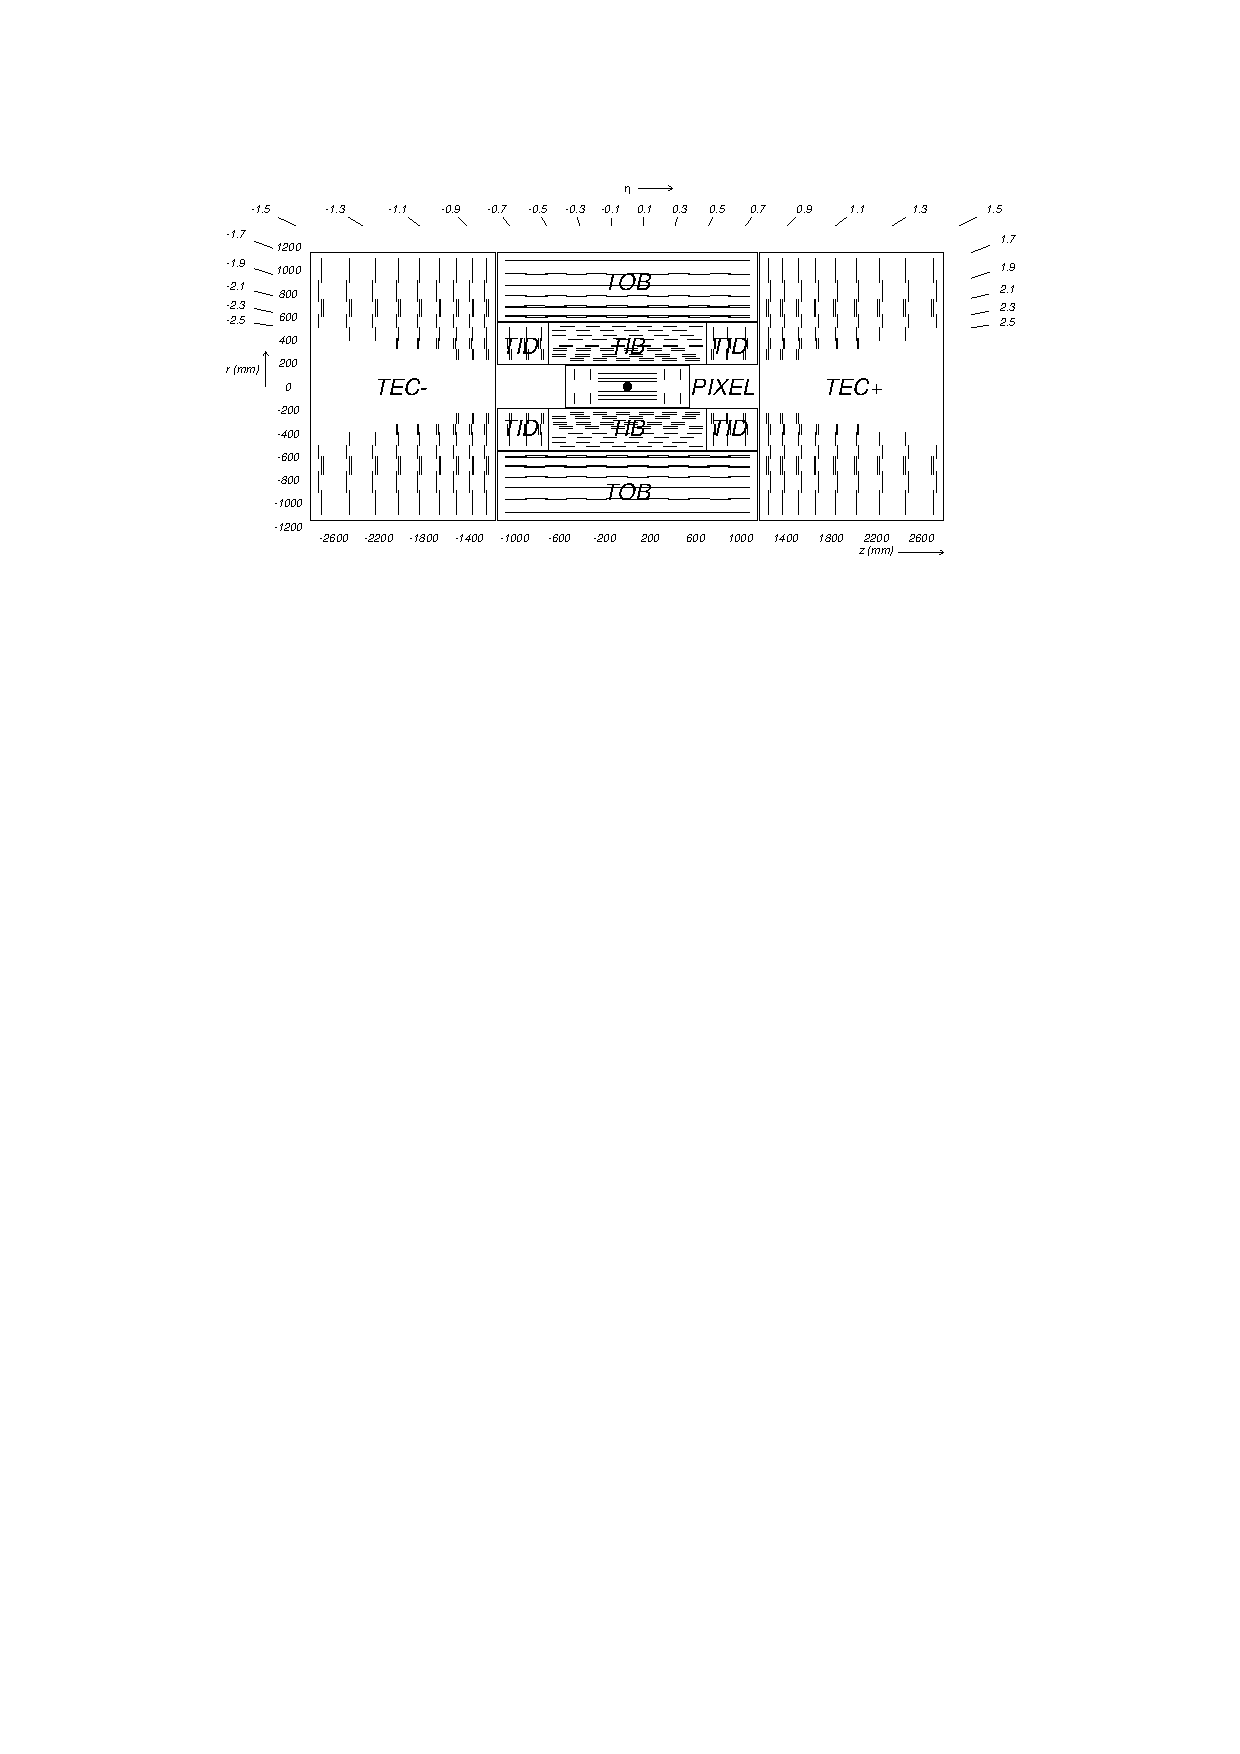
\includegraphics[scale = 1.1]{/home/anter/Desktop/Thesis/Figures/cropped_Tracker.pdf}\\
\caption[The longitudinal section of the inner tracking system.]{The longitudinal section of the inner tracking system consisting of the silicon pixel detector and the silicon strip detector is shown in $r$-$z$ plane. The silicon strip detector has four components : The Tracker Inner Barrel (TIB) complemented by the Tracker Inner Disks (TID) which are further surrounded by the Tracker Outer Barrel (TOB) in barrel region. Tracker End Cap (TEC) covers high $\eta$ ranges up to $\eta$ = 2.5. Taken from \cite{Chatrchyan:2008aa}.}
\label{fig:tracker}
\end{center}
\end{figure}
The active silicon area of CMS tracker is about 200m$^{2}$ which makes it the largest silicon tracker. Along with the measurement of tracks, the energy also needs to be measured for which the calorimeters are present outside the tracker. The tracker should interfere with the particles to a minimum extent so that their momentum can be measured precisely but to measure their energy, they are required to interact with the calorimeters fully.

\subsection{Electromagnetic Calorimeter}
The electromagnetic calorimeter (ECAL) is a homogeneous and hermetic calorimeter used to slow down the produced photons and electrons/positrons and measure their energy by absorb them into the detector material. ECAL consists of 61200 lead tungstate (PbWO$_4$) crystals in the barrel part and 7324 crystals in each of the two endcaps. PbWO$_4$ is a very dense material with a short radiation length of X$_0$ = 0.89 cm and covers the pseudorapidity up to $|\eta|$ \ls 3.0. The particles interact with matter and produce electromagnetic shower through the subsequent processes of bremsstrahlung and electron-positron pair production. The energy of the particles deposited by Compton scattering and the photoelectric effect causes excitation of the material atomic state and the emission of photons. These photons are detected by silicon avalanche photo diodes (APDs) in the barrel region and vacuum phototriodes (VPT) in the end-cap region. The number of created photons gives the direct measure of energy of the incident particle. The incorporation of oxygen makes it highly transparent and enables to emit scintillation light. The small Moli$\grave{e}$re radius of 2.19 cm gives a fine granularity. These properties leads to compact size of ECAL and can be placed easily within the solenoid magnet. 

Figure~\ref{fig:ecal} presents a geometric view of ECAL in the $y$-$z$ plane showing the arrangement of different parts of ECAL 
: the ECAL barrel (EB) extending up to $|\eta|$ \ls 1.479 using more than 60000 crystals and ECAL endcaps (EE) covering the region 1.479 \ls $|\eta|$ \ls 3.0 with an additional 15000 crystals. The preshower detectors (ES) made of lead absorbers and silicon detectors are put in front of the endcaps to distinguish high energetic single photons from low energetic photon pairs originating from neutral pions decays.

\begin{figure}[!h]
\begin{center}
\vspace*{3mm} 
\hspace*{-5mm}
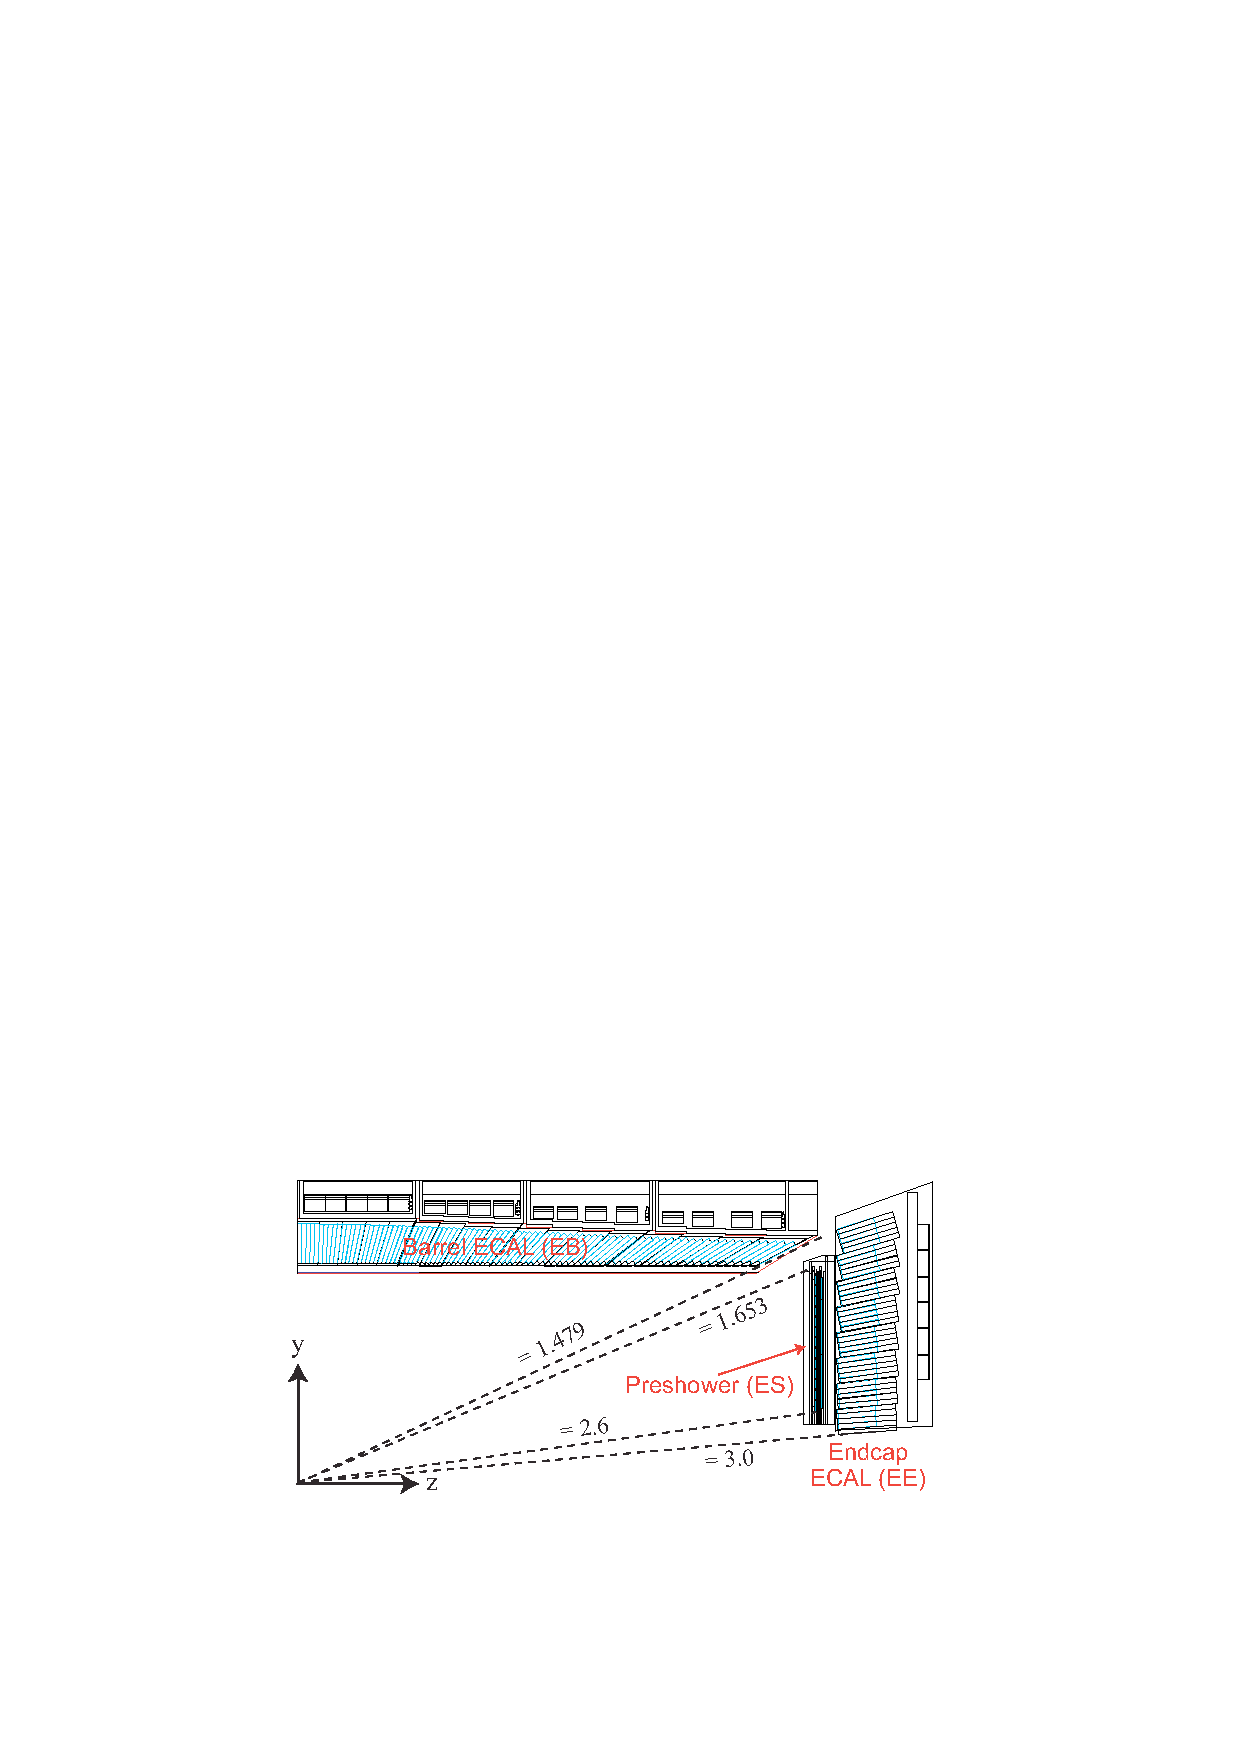
\includegraphics[scale = 1.2]{/home/anter/Desktop/Thesis/Figures/cropped_ECAL.pdf}\\
\vspace*{2mm}
\caption[A geometric view of one quarter of the electromagnetic calorimeter (ECAL) in $y$-$z$ plane.]{A geometric view of one quarter of the electromagnetic calorimeter (ECAL) in $y$-$z$ plane showing the arrangement of sub-modules covering the barrel region (EB) and the endcaps (EE). ECAL is complemented with preshower detector (ES) mounted in front of the endcaps. Taken from \cite{Bayatian:2006nff}.}
\label{fig:ecal}
\end{center}
\end{figure}

The relative energy resolution of the ECAL has been measured to be \cite{Adzic:2007mi} :

\begin{equation}
{\rm \bigg(\frac{\sigma(E)}{E}\bigg)^2 = \bigg(\frac{2.8\%}{\sqrt{E}}\bigg)^2 \plus \bigg(\frac{12\%}{E}\bigg)^2 \plus \bigg(0.30\%\bigg)^2}
\end{equation}
where E is the energy in GeV. The first term is the stochastic component caused by fluctuations in lateral shower containment and in the energy deposited in the preshower absorber. The second term is the contribution by noise and the last is the constant term comes from the non-uniformity of the longitudinal light collection, inter-calibration errors, and leakage of energy from the back of the crystal.

\subsection{Hadronic Calorimeter}
At CMS, the major fraction of the produced particles in proton-proton collisions is hadrons. The combined CMS calorimeter system measures directions and energies of quarks, gluons and neutrinos by measuring the energy and direction of particle jets. The neutral hadrons do not leave track and hence their energy is measured by taking into account the missing transverse energy (\ETmiss). The determination of \ETmiss is a crucial tool in searching the new particles and phenomena. The hadron calorimeter (HCAL) are particularly important in the identification of hadron jets, neutrinos as well as electrons, photons and muons in conjunction with the ECAL and the muon system. Hence HCAL is an essential sub-system of the CMS detector and contributes to most of CMS's physics studies.

HCAL is a sampling calorimeter installed inside the solenoid coil. It is made up of non-magnetic brass absorber having a short interaction length of $\lambda_I$ = 16 cm interleaved with plastic scintillators having wavelength-shifting (WLS) fibres as readout. The hadrons produced with high energy showers a large number of pions and nucleons by inelastic interactions. The hadronic shower spreads more than the electromagnetic showers because of large transverse momentum of the secondary particles. As the energy of the particles is lower than a certain threshold, the ionization and low-energy hadronic processes come into play. The active scintillation material gets excited and emits blue-violet light. 
\begin{figure}[!h]
\begin{center}
\vspace*{3mm} 
\hspace*{-5mm}
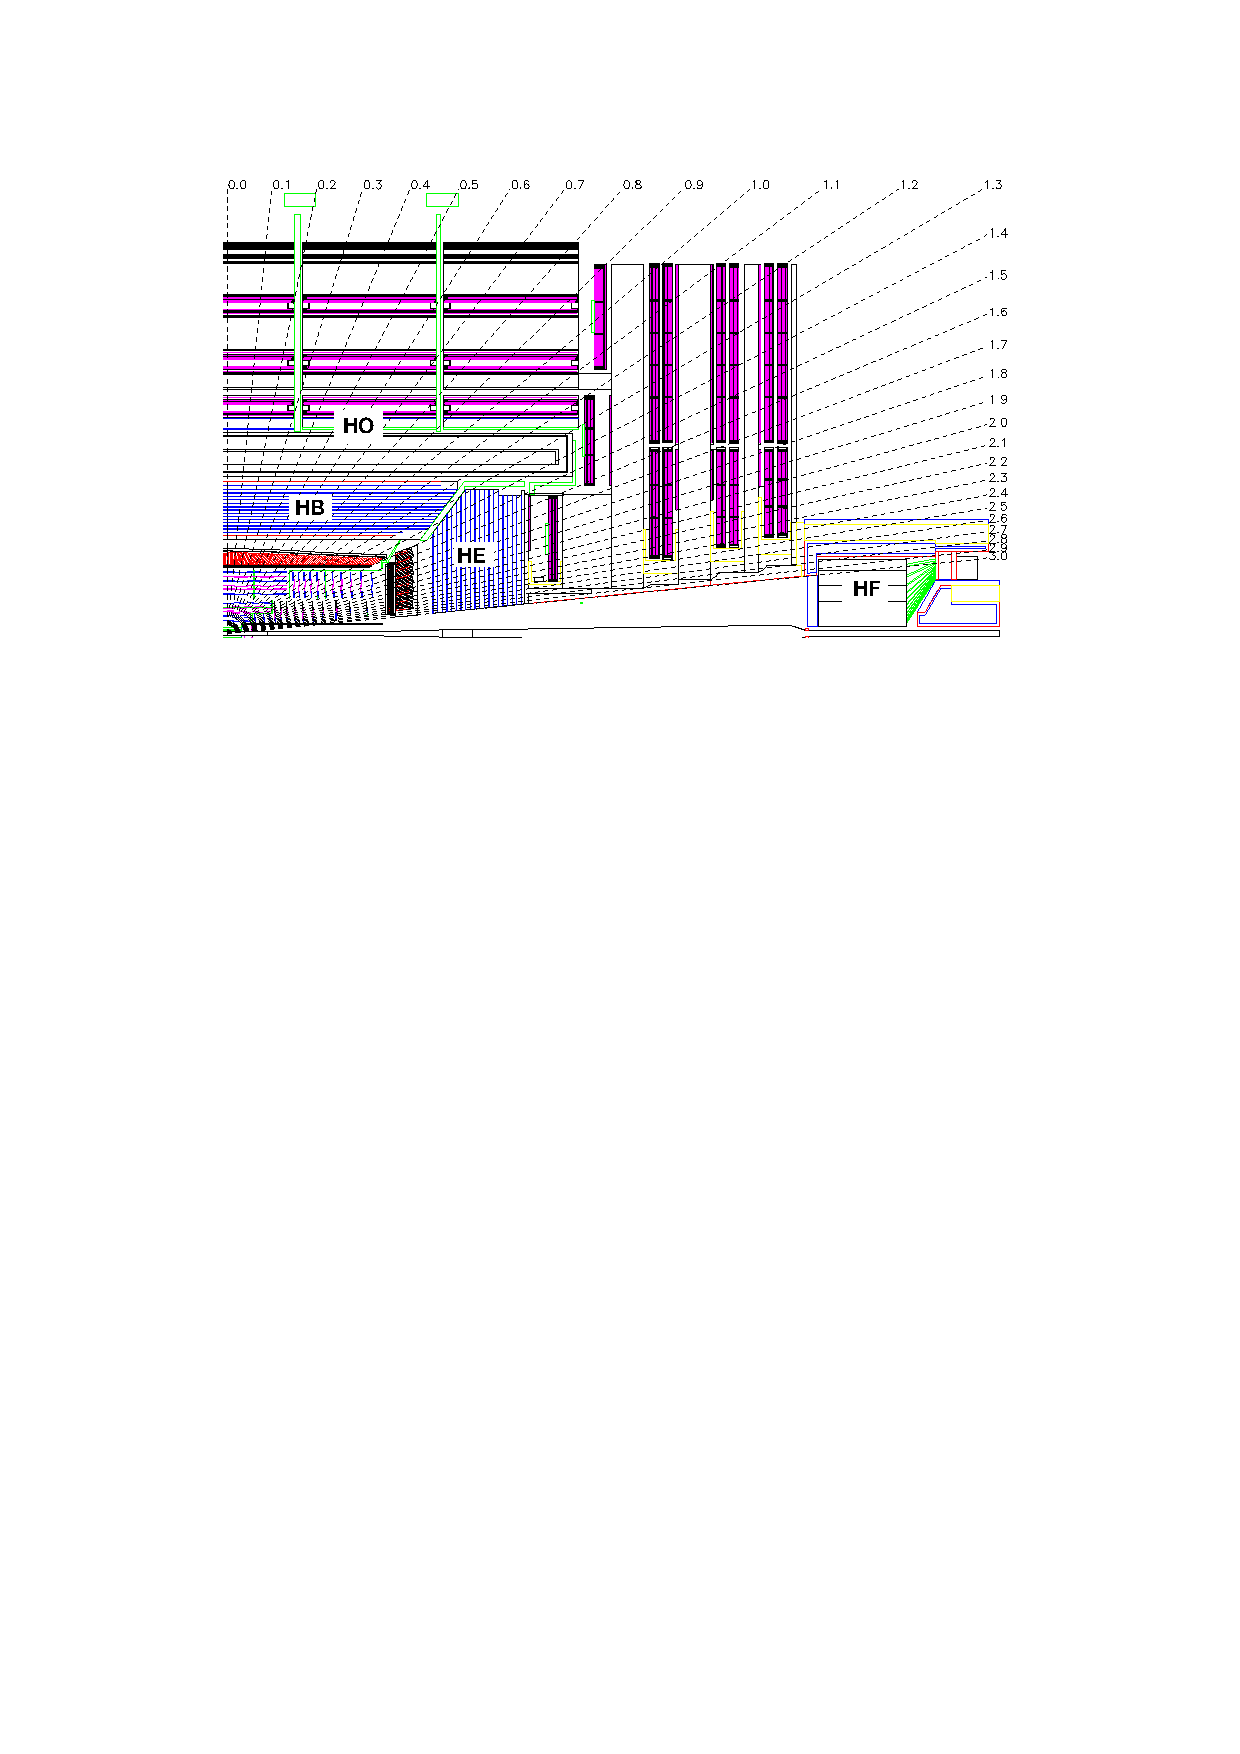
\includegraphics[scale = 1.]{/home/anter/Desktop/Thesis/Figures/edited_cropped_HCAL.pdf}\\
\vspace*{4mm}
\caption[Longitudinal view of one quarter of the hadronic calorimeter (HCAL) detector in $r$-$\eta$ plane.]{Longitudinal view of one quarter of the hadronic calorimeter (HCAL) detector in $r$-$\eta$ plane showing its different parts : hadron barrel (HB), hadron outer (HO), hadron endcap (HE) and hadron forward (HF). Taken from \cite{Chatrchyan:2008aa}.}
\label{fig:hcal}
\end{center}
\end{figure}
All scintillators are connected to photodiodes using wavelength shifters which read out the signals and pass them to the data acquisition system. The longitudinal view of one quarter of the HCAL presented in Fig.~\ref{fig:hcal} shows the different parts : \\\newline
{\bf Hadron Barrel -} The hadron barrel (HB) is divided into two identical half barrel sections on either side of the interaction point. Each half barrel is made of 18 azimuthal wedges which are further divided into four azimuthal sectors each giving a granularity of $\Delta\phi$ = 0.087. In $z$ direction, the plastic scintillators are divided into 16 intervals of granularity $\Delta\eta$ = 0.087. HB covers the region up to $|\eta|$ \ls 1.305 and overlaps with endcaps for 1.305 $\leq~|\eta|~\leq$ 1.392. Since HB has the highest resolution $(\Delta\eta~\times~\Delta\phi = 0.087~\times~0.087$), it constitute the optimal region for a data-driven calibration of the jet energy scale. The thickness of the HCAL amounts to 7-11 interaction lengths and which should sufficient enough to stop nearly all hadrons in the calorimeter.\\\newline
{\bf Hadron Outer -} The total amount of material in barrel region to absorb the hadronic shower is not sufficient. This requirement is fulfilled by placing an outer hadron (HO) calorimeter as a tail catcher on top of the coil of the magnet. The HO utilizes the solenoid coil as an additional absorber equal to 1.4/sin$\theta$ interaction lengths and measures the tails of hadron showers penetrating the HB and the coil. Since the HO is physically located inside the muon system, it is strongly constrained by its geometry. The muon system is subdivided into 5 rings along the $z$-axis. Each of these rings is 2.536 m wide in $z$-direction and the HO is placed as first sensitive layer in these rings, with a scintillator thickness of 10 mm. The central ring ($\eta$ = 0) has two scintillator layers placed on each side of 19.5 cm thick iron layer.\\ \newline
{\bf Hadron Endcap -} The hadron endcaps (HE) extends the pseudorapidity range up to $|\eta|$ \ls 3.0, a region containing about 34\% of the particles produced in the final state The granularity in $\Delta\eta~\times~\Delta\phi$ is 0.087 $\times$ 0.087 up to $|\eta|$ \ls 1.6 and 0.17 $\times$ 0.17 for $|\eta|$ \gr 1.6. The usage of non-magnetic material in order to not disturb the magnetic field and the close distance to the beam line were the main challenges faced during the construction of the HE. The continuous radiation damages decrease the detector response which need to be corrected and monitored at regular intervals. \\ \newline
{\bf Hadron Forward -} The hadron forward (HF) calorimeter lies 2.8 \ls $|\eta|$ \ls 5.2 region and is placed more closer to the beam pipe at distance of $z$ = $\pm$11.2 m from the interaction point. It is essentially a cylindrical steel structure with an outer radius of 130.0 cm which is azimuthally subdivided into 36 20$\degree$ modular wedges. The HF is made of 5 mm thick grooved steel plates which have quartz fibers inserted into the grooves. The fibres run parallel to the beam line which are bundled to form 0.175 $\times$ 0.175 ($\Delta\eta~\times~\Delta\phi$) towers. HF detects the jets with very high $\eta$ and the hadronization products of the beam remnants. It is built using iron absorbers and quartz fibers as active material, which measures the emitted Cerenkov light and produces the signal in the photomultipliers (PMT).

%HCAL provides the energy and direction measurements of the jets in conjunction with ECAL system. It measures the total visible and missing transverse energy due to hermetic coverage.
The relative hadronic energy resolution of the barrel HCAL and ECAL combination can be parametrized as :
\begin{equation}
{\rm \bigg(\frac{\sigma(E)}{E}\bigg)^2 = \bigg(\frac{a}{\sqrt{E}}\bigg)^2 \plus b^2}
\end{equation}
with a stochastic term a and a constant term b. These values have been measured \cite{Chatrchyan:2009ag} as a = (0.847$\pm$0.016) $\sqrt{\rm GeV}$ and b = 0.074 $\pm$ 0.008 whereas for HF the measured values are a = 1.98 $\sqrt{\rm GeV}$ and b = 0.09.

\subsection{Superconducting Magnet}
The superconducting magnet is the key feature of the CMS detector which is 13m long and 6m in diameter. Its refrigerated superconducting high-purity aluminium-stabilized niobium-titanium coils cooled at 4 Kelvin produces a magnetic field of 4 Teslas (T). The magnet will run at 3.8 T in order to maximize its lifetime. This intense solenoidal field makes the compactness and cylindrical symmetry of the detector possible. The magnet is placed between the calorimeters and the muon system. The solenoidal magnetic field parallel to the beam bends the tracks of the high momentum charged particles in the transverse plane. The curvature of the trajectory increases with the strength of the magnetic field which make possible to determine the transverse momentum more precisely. The magnet is complemented by a $\sim$10000 tonnes iron yoke which returns the magnetic field at 2 T.

\subsection{Muon System}
As the name suggests, the detection of muons is of central importance to CMS. Only the muons and neutrinos, out of all the known stable particles, pass through the calorimeter without depositing most or all of their energy. They interact very little with matter and can travel long distances through the dense matter. The charged muons can be detected by having an additional tracking system outside the calorimeters whereas the neutrinos are practically undetectable as they escape completely without being tracked in any of the layers. Their presence can be detected from the missing energy carried by them. The CMS muon system is installed outside calorimeters in the iron return yoke of the magnet. The muon system perform the muon identification, momentum measurement and triggering. Good muon momentum resolution and trigger capability are enabled by the high-field solenoidal magnet and its flux-return yoke. The latter also serves as a hadron absorber for the identification of muons. The CMS muon system is designed to have the capability of reconstructing the momentum and charge of muons over the entire kinematic range of the LHC. The muon system shown in Fig.~\ref{fig:muon} consists of three types of gaseous particle detectors : \\ \newline
\begin{figure}[!h]
\begin{center}
\vspace*{3mm} 
\hspace*{-5mm}
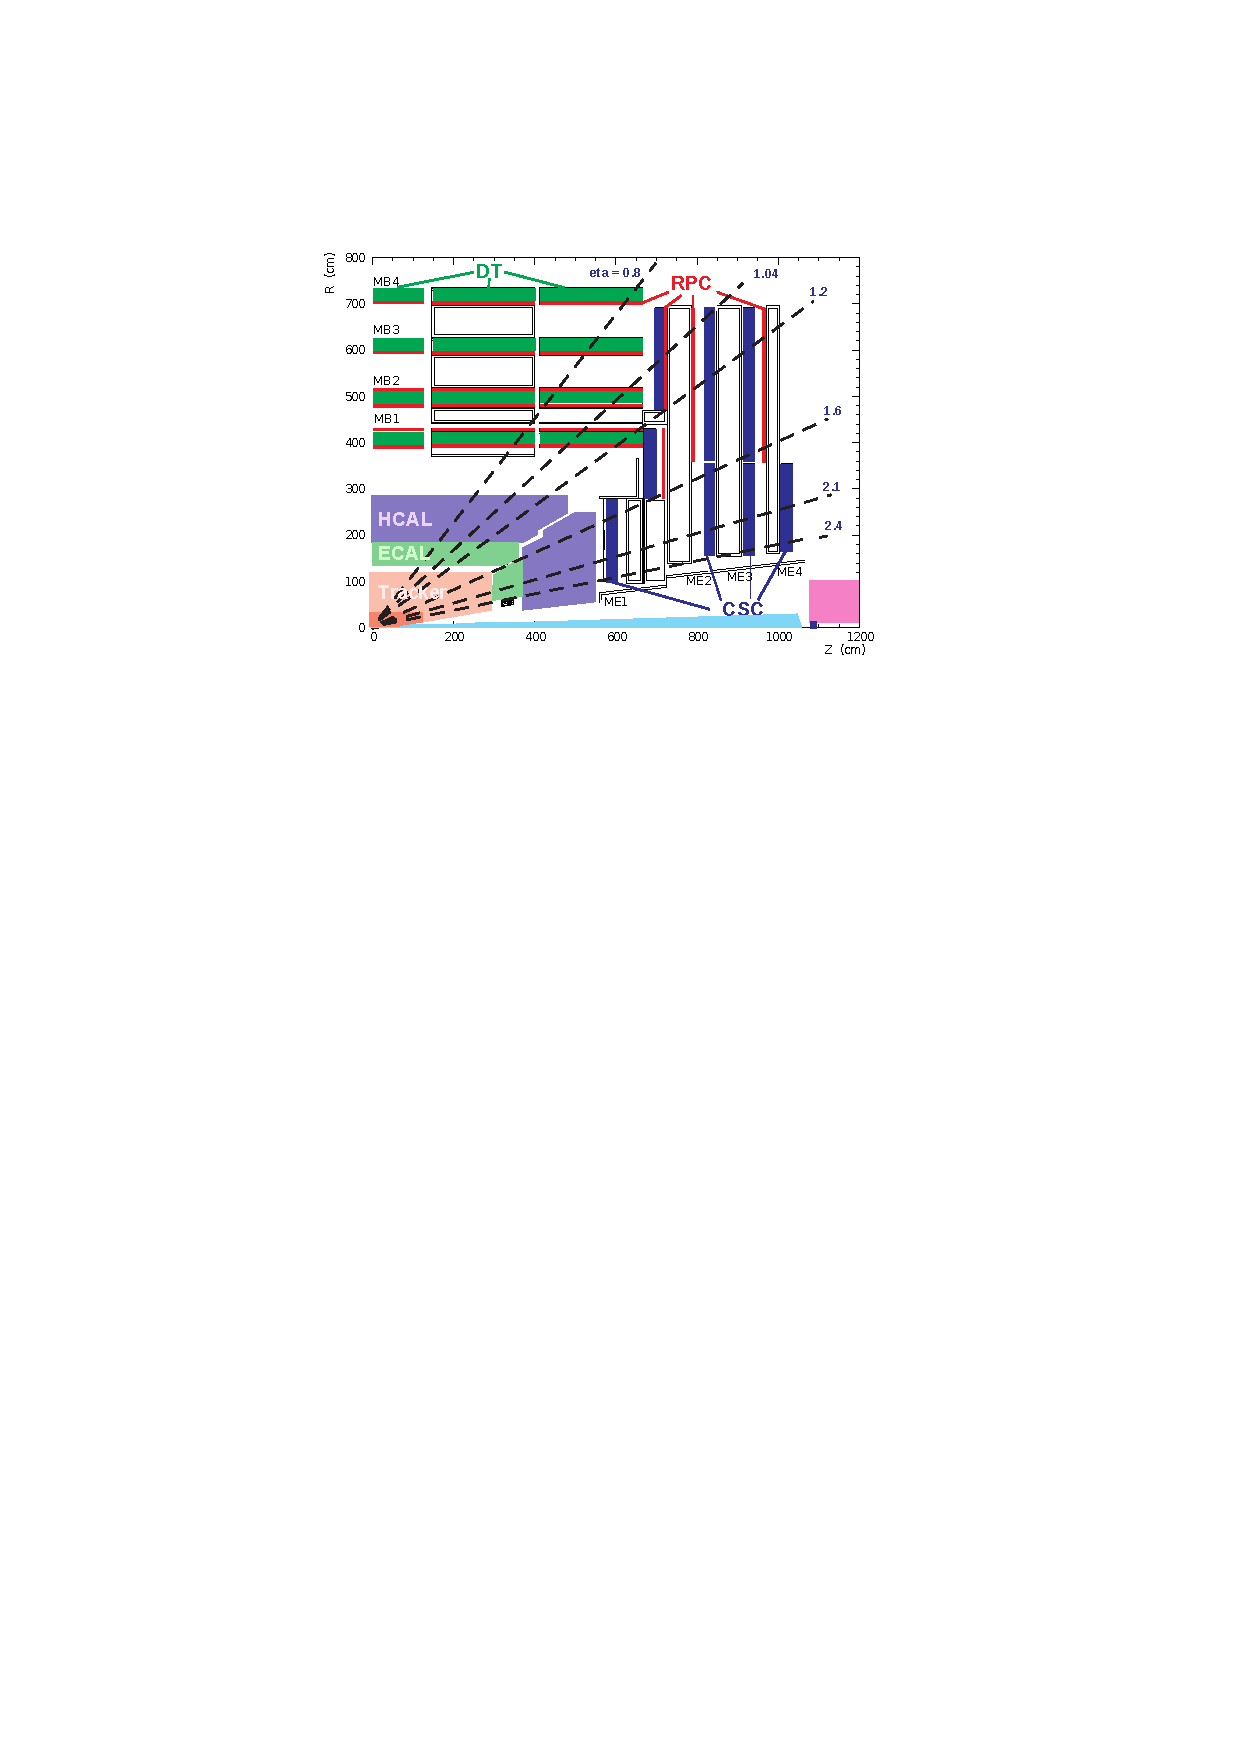
\includegraphics[scale = 1.4]{/home/anter/Desktop/Thesis/Figures/cropped_Muon.pdf}\\
\vspace*{4mm}
\caption[A longitudinal view presenting the location of the three muon sub-systems.]{A longitudinal view presenting the location of the three muon sub-systems : four Drift Tube (DT) stations in the barrel (MB1-MB4, green), four stations of Cathode Strip Chambers (CSC) in the endcap (ME1-ME4, blue), and the Resistive Plate Chambers (RPC) stations (red)\footnotemark.}
\label{fig:muon}
\end{center}
\end{figure}
{\bf Drift Tube -} 
The muon barrel (MB) detector has four concentric layers of drift tube (DT) chambers inside the iron yoke which covers the region up to $|\eta|$ \ls 1.2. DT stations are distributed into 5 wheels along the $z$ direction. Each wheel is divided into 12 sectors, each covering a 30$\degree$ azimuthal angle. The DTs are aluminium tubes of 2.5 m of length and 4.2 $\times$ 1.3 cm$^{2}$ of area, filled with gas mixture ( 58\% Ar \plus 15 \% CO$_{2}$). \\ \newline \footnotetext{Source : \url{https://arxiv.org/abs/1209.2646}}
{\bf Cathode Strip Chambers -} In the forward region, the muon and background flux is higher. So cathode strip chambers (CSC) are preferred because of their fast response time, radiation tolerance and fine segmentation. The four stations of CSCs are installed in each end cap covering in total the region of 0.9 \ls $|\eta|$ \ls 2.4. Each CSC is trapezoidal in shape and consists of 6 gas gaps, each gap having a plane of radial cathode strips and a plane of anode wires running almost perpendicularly to the strips. \\ \newline 
{\bf Resistive Plate Chambers -} Both DT and CSC are accompanied by resistive plate chambers (RPC) which are double-gap chambers, operated in avalanche mode to ensure good operation at high rates. They help to resolve ambiguities in attempting to make tracks from multiple hits in a chamber and provide additional points for determination of a muon trajectory. They provide fast response to the trigger system which is described in the following section.
 
\subsection{Trigger and Data Acquisition System}
The proton-proton collisions (events) take place at high interaction rates at LHC. In the 2012 run period, at beam crossing frequencies of 25 ns there are 40 million bunch crossings per second with an average of around 20 collisions per bunch crossing. Both the collision and the overall data rates are much higher than the rate at which the information can be stored. So a dramatic rate reduction has to be achieved which is possible with an efficient trigger system by retaining interesting signal events and rejecting background events. The decision of accepting or rejecting an event has to be performed very quickly and it is based on signals of certain physics objects inside the detector.
CMS has a two-level complex trigger system : \\\newline
{\bf Level-1 Trigger -} The Level-1 (L1) trigger system is based on custom electronics which stores the events at maximum rate of 100 kHz and then forward them to the next level triggers. The L1 system uses only coarsely segmented data from calorimeter and muon detectors, while holding all the high-resolution data in pipeline memories in the front-end electronics. Figure~\ref{fig:L1} shows the work flow of the L1 trigger system. 
\begin{figure}[!h]
\begin{center}
\vspace*{3mm} 
\hspace*{-5mm}
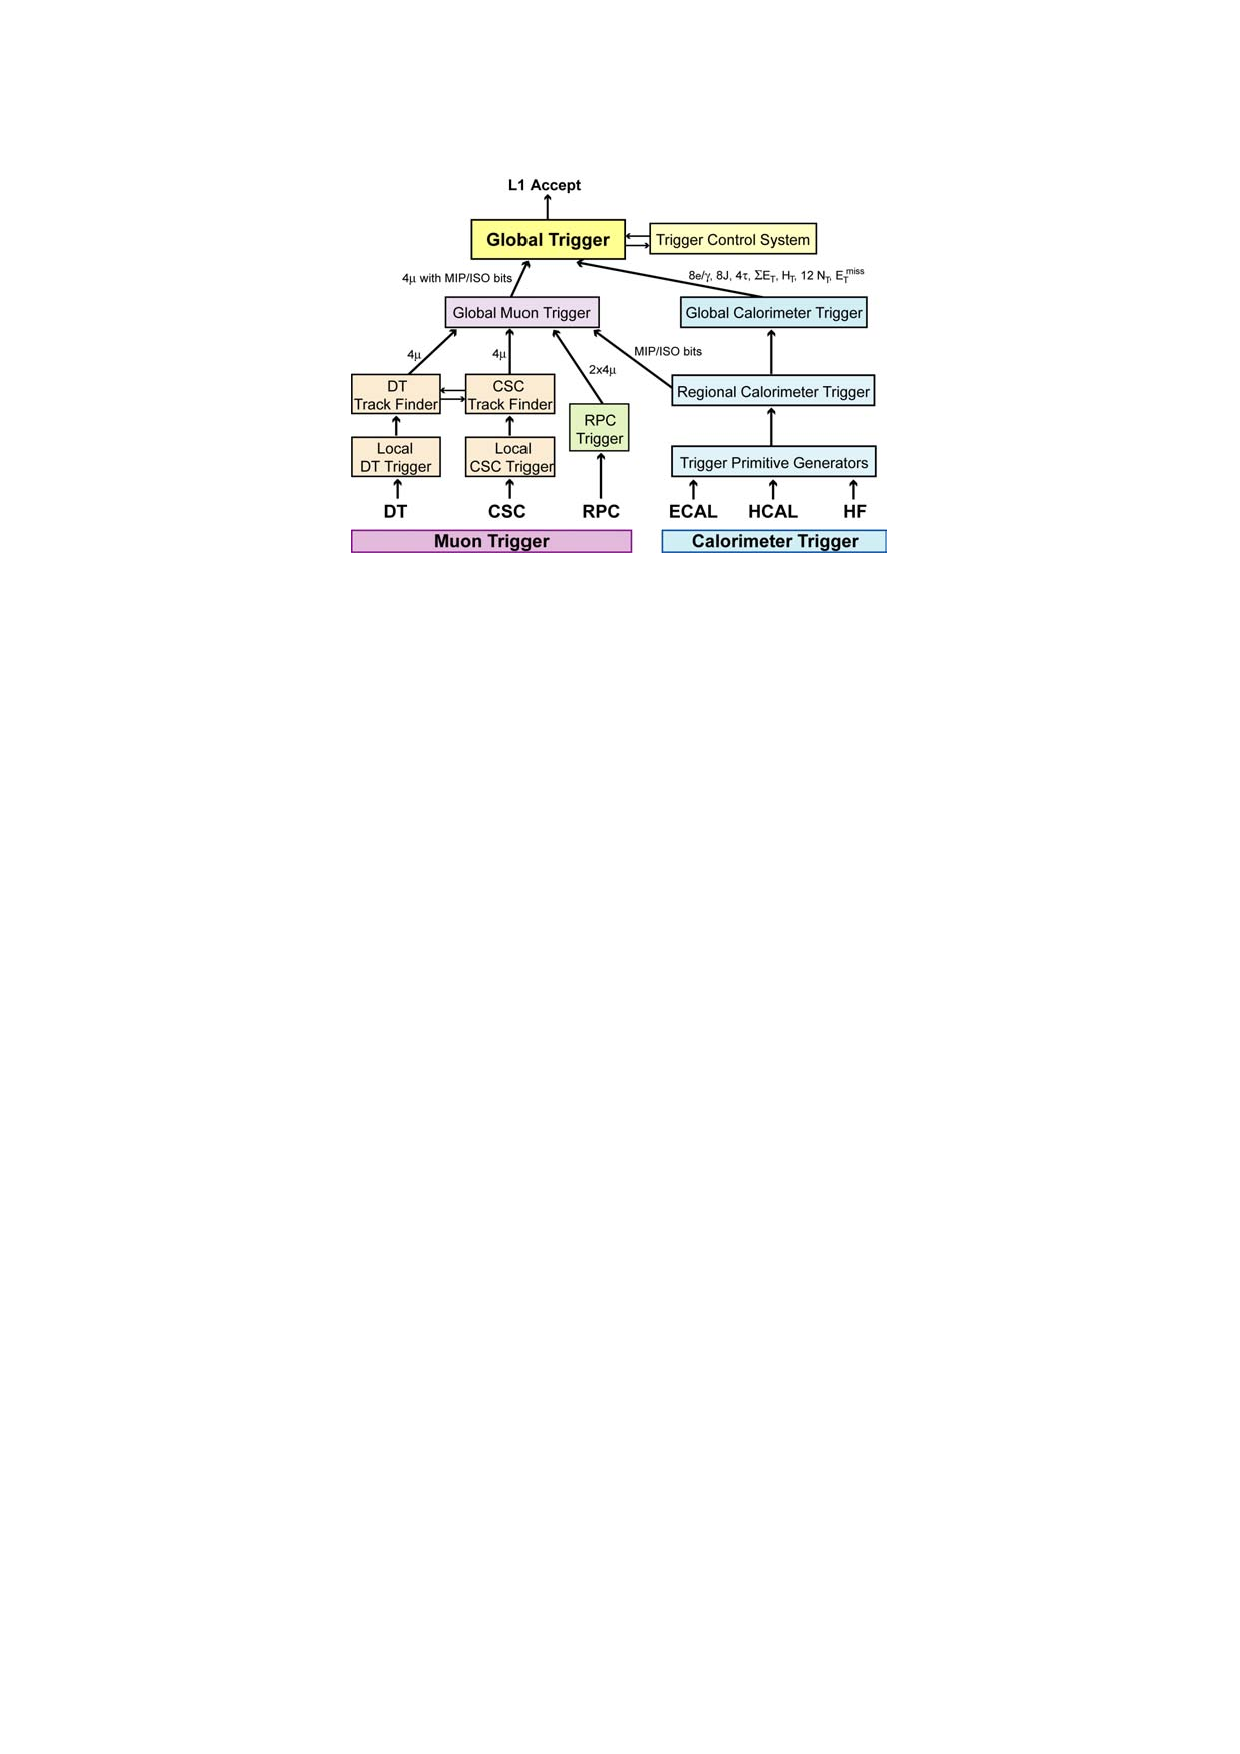
\includegraphics[scale = 1.5]{/home/anter/Desktop/Thesis/Figures/cropped_Trigger.pdf}\\
\vspace*{4mm}
\caption[Work flow of the L1 trigger system]{Work flow of the L1 trigger system. Taken from \cite{Chatrchyan:2008aa}.}
\label{fig:L1}
\end{center}
\end{figure}
L1 trigger consists of local, regional and global components. The local triggers known as Trigger Primitive Generators (TPG), are based on energy deposits in calorimeter trigger towers and tracks in muon chambers. Regional Triggers combine their information and use pattern logic to determine ranked and sorted trigger objects such as electron or muon candidates in limited spatial regions. The rank is determined as a function of energy or momentum and quality, which reflects the level of confidence attributed to the L1 parameter measurements, based on detailed knowledge of the detectors and trigger electronics and on the amount of information available. The Global Calorimeter and Global Muon Triggers determine the highest-rank calorimeter and muon objects across the entire experiment and transfer them to the Global Trigger, the top entity of the Level-1 hierarchy. The latter takes the decision to reject an event or to accept it for further evaluation by the HLT. \\\newline
{\bf High Level Trigger -} At the second step, a software-based High-Level Trigger (HLT) is designed to reduce the maximum L1 accept rate of 100 kHz to a final output rate of 100 Hz. The HLT system filter events by performing physics selections using faster versions of the offline reconstruction software. The HLT is provided by a subset of the on-line processor farm which, in turn, passes a fraction of the accepted events to the Data Acquisition (DAQ) system for more complete processing.

\subsubsection{Jet Triggers}
\begin{comment}
\begin{figure}[!h]
\begin{center}
\vspace*{3mm} 
\hspace*{-5mm}
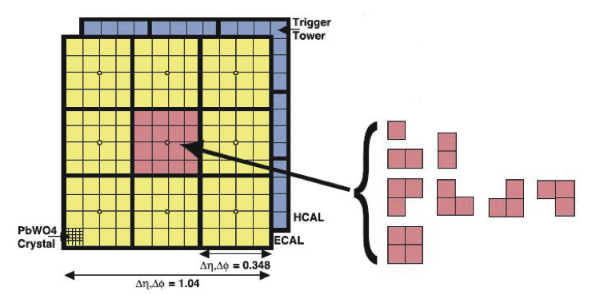
\includegraphics[scale = 0.7]{/home/anter/Desktop/Thesis/Figures/Jet_trigger.png}\\
\vspace*{4mm}
\caption[Muon]{Illustration of the available tower granularity for the L1 jet finding algorithm in the
central region, |η|<3 (left). The jet trigger uses a 3×3 calorimeter region sliding window technique which spans the full(η,φ)coverage of the calorimeter. The active tower patterns allowed for L1τjet candidates are shown on the right Work flow of the L1 trigger system \cite{Chatrchyan:2008aa}.}
\label{fig:Jettrigger}
\end{center}
\end{figure}
\end{comment}
Triggers based on jet and missing transverse energy (\ETmiss) triggers are important for search for new physics whereas the single-jet triggers are mainly designed to study quantum chromodynamics (QCD). In this thesis, the single-jet triggers are used to select the events for analysis. At L1, they use mainly information from the calorimeter by looking for an energy cluster and a high energy deposit. The sums of transverse energy from ECAL and HCAL are computed in 4 $\times$ 4 trigger towers, except in the HF region where this quantity is measured in the whole trigger tower itself. If this deposit is greater than a certain threshold, the event is selected at L1 and it is passed to the HLT. Jets are reconstructed in the HLT using the anti-\kt jet clustering algorithm. The inputs for the jet algorithm are either calorimeter towers giving ``CaloJet'' objects, or the reconstructed particle flow objects giving ``PFJet'' objects. The processing time of reconstruction algorithm is high and hence the jet trigger paths are divided into multiple selection steps. At first, jets are reconstructed from calorimeter towers. Only for events in which at least one calorimeter jet passes a certain \pt threshold, the particle flow algorithm is run and the jets are clustered again from the particle flow candidates. In 2012, most of the jet trigger paths use PFJets as their inputs. The rate of jet events is quite high, so PFJet trigger paths have a pre-selection based on CaloJets. The matching between CaloJets and PFJets is required in single PFJet paths. Due to the flexibility of the HLT, it is possible to apply the jet energy corrections during the HLT selection.

\subsubsection{Data Acquisition System}
As the L1 trigger accepts events at a rate of 100 kHz, the Data Acquisition (DAQ) system has to process the events at the same speed. It reads out the data of all detector sub-components and assembles the complete events, see Fig.~\ref{fig:DAQ}. The data is subsequently passed to the HLT which further reduces the rates to a few hundred events per second. Finally, the events are merged and saved to a local storage system, from which they are continuously transferred to the Tier-0 computing center at CERN.

\begin{figure}[!h]
\begin{center}
\vspace*{3mm} 
\hspace*{-5mm}
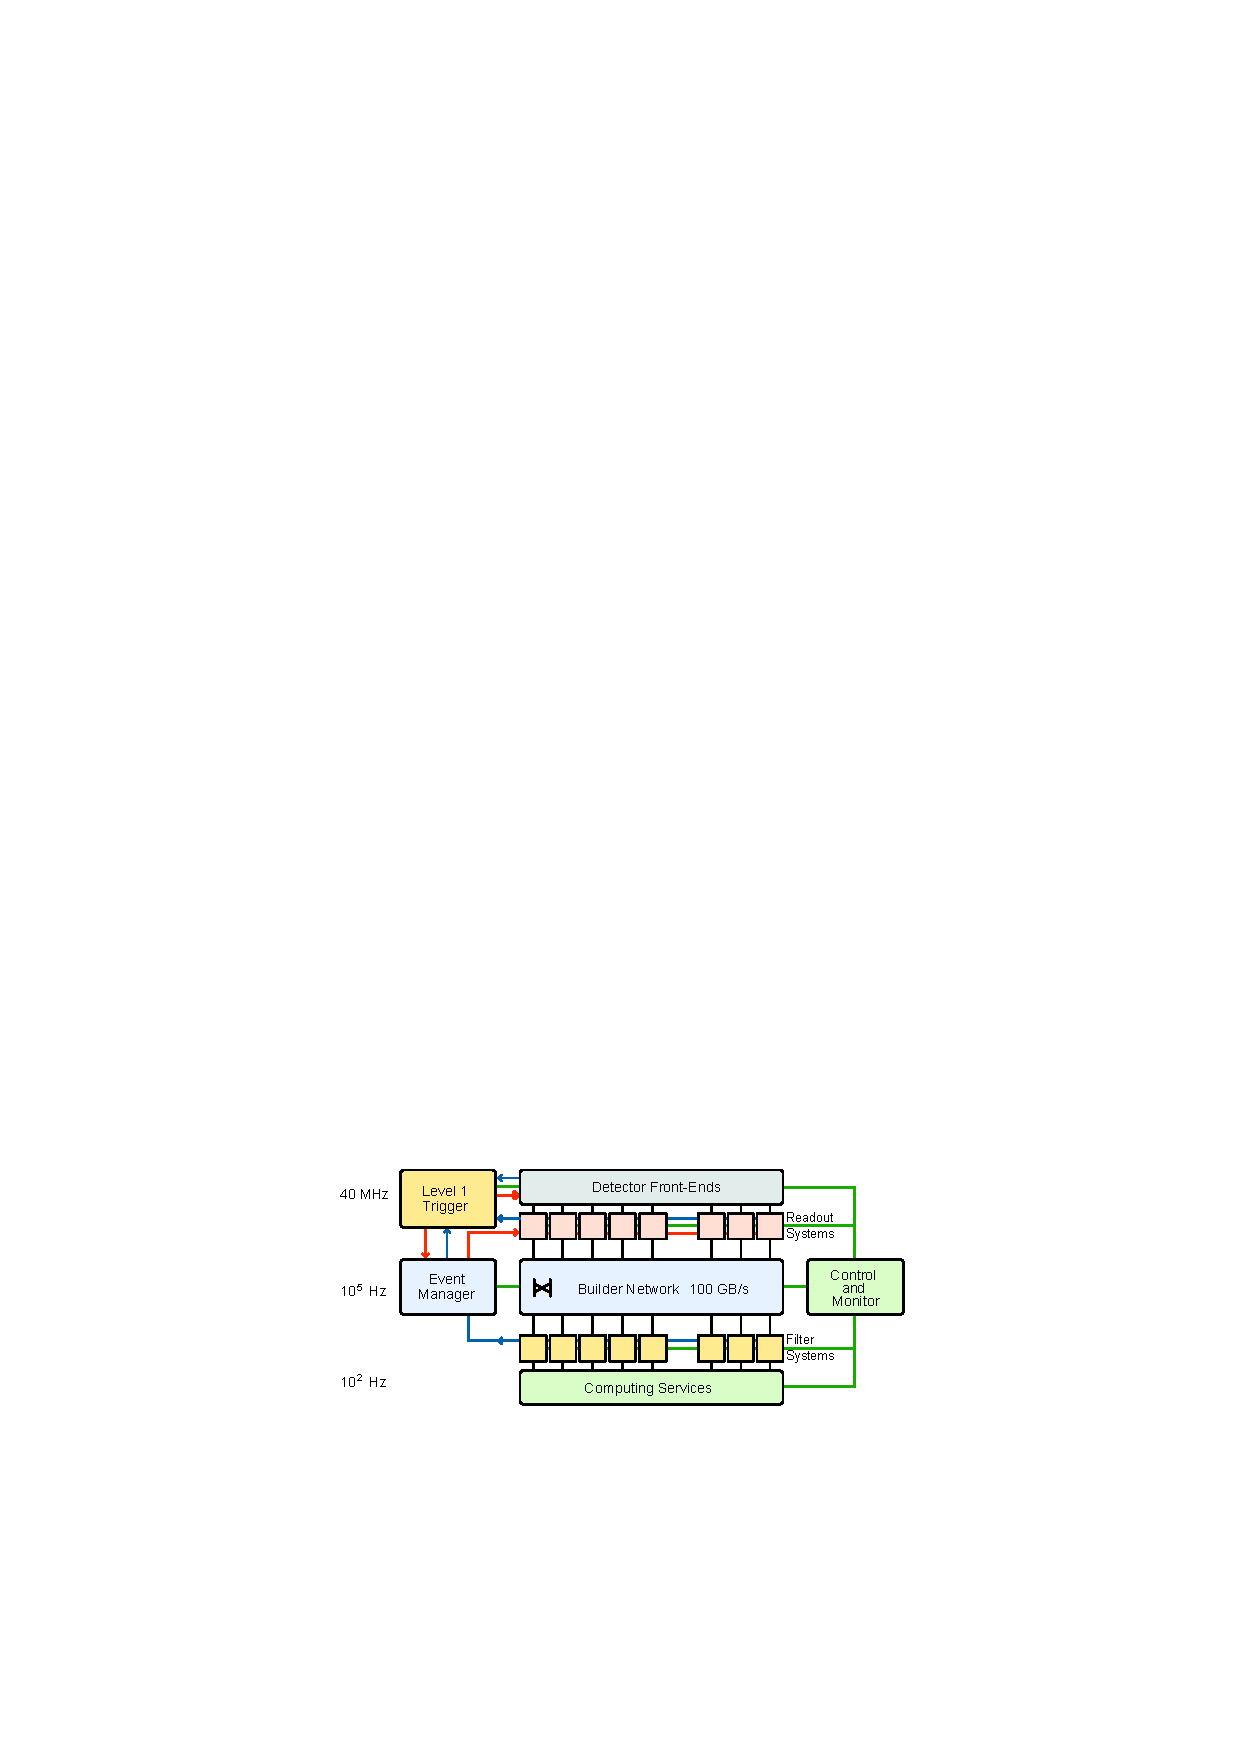
\includegraphics[scale = 1.3]{/home/anter/Desktop/Thesis/Figures/cropped_DAQ.pdf}\\
\vspace*{4mm}
\caption[Architecture of the CMS DAQ system.]{Architecture of the CMS DAQ system. Taken from \cite{Chatrchyan:2008aa}.}
\label{fig:DAQ}
\end{center}
\end{figure}

\subsection{Data Management}
Although the trigger system reduces the collision rate enough to be stored in tape, still there is a huge amount of data need to be analyzed. An efficient computing infrastructure and the software is required for storing and distributing the data. To meet this need, the LHC has a data storage infrastructure called the Worldwide LHC Computing Grid (WLCG) \cite{Bird:2005js}. WLCG provides a hierarchical structure, as shown in Fig.~\ref{fig:Computing}, in a series of four levels or Tiers. Each Tier is made up of several computer centres. All the raw collision data collected by CMS is converted into a format suitable for offline analysis and sorted in the form of data sets at the Tier-0 site at CERN. This processed data is then transferred to Tier-1 centers all over the world where reconstruction algorithms are run. Further reconstructed and simulated data is distributed to Tier-2 sites, where it is available for physics analysis mainly performed on Tier-3 sites. %The powerful Monte Carlo event generators are required to simulate the collision events and these are dicussed in the next chapter.

\begin{figure}[!h]
\begin{center}
\vspace*{3mm} 
\hspace*{-5mm}
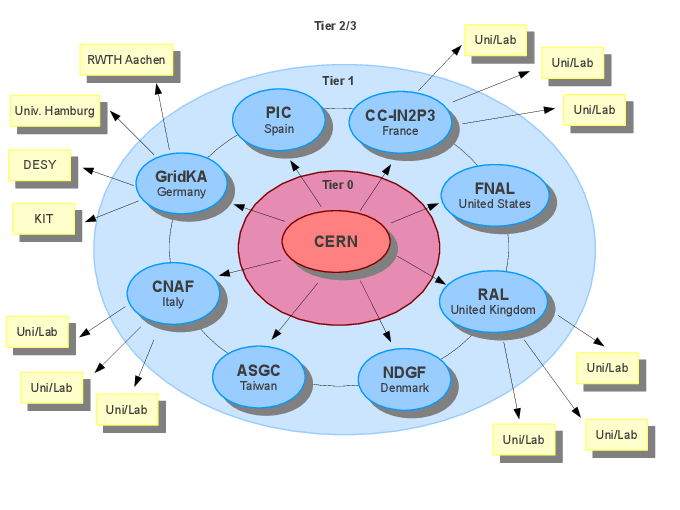
\includegraphics[scale = 0.95]{/home/anter/Desktop/Thesis/Figures/Computing.png}\\
\vspace*{4mm}
\caption[Schematic overview of the CMS computing grid.]{Schematic overview of the CMS computing grid. All data collected by CMS is stored at the Tier-0 site at CERN which is then transferred to Tier-1 centers all over the world. Further reconstructed and simulated data is distributed to Tier-2 sites, where it is available for physics analysis mainly performed on Tier-3 sites. Taken from \cite{Bird:2005js}.}
\label{fig:Computing}
\end{center}
\end{figure}

\section{Software Tools}
Every year, the CMS is recording a huge amount of data, from collisions as well as simulations. This data is analyzed iteratively to improve the understanding of the detector and the measured physics. So a dedicated data structure and software tools are required for data analysis. These are included in the software framework referred to as CMSSW. This section describes the CMSSW framework and software tools used in the current study.

%CMSSW has also some pre-defined data tier, i.e sets with specific objects. Among them are the data tier RECO which included all reconstructed data objects, whereas the data tier AOD (Analysis Object Data) is only a subset with physical objects needed for a particular analysis.
\subsection{CMSSW Framework}
The CMS software framework (CMSSW) \cite{CMS:2005aa} provides all necessary tools for a physics analysis. The CMSSW framework is built on top of an event data model (EDM). It is a container for arbitrary C\plusn\plus objects, e.g. recorded raw data and reconstructed physical objects (e.g particles, missing transverse energy) or derived quantities of an event. The reconstruction and distribution algorithms in CMSSW are divided into modules, which can be dynamically loaded and run. The CMSSW event processing model consists of one executable, called cmsRun, and many plug-in modules which are managed by the framework. SCRAM (Source Configuration, Release, And Management) is a configuration and management tool in the framework. It builds a runtime environment and make available all the necessary shared libraries. The shared libraries reduces memory consumption by only loading required modules during runtime. The CMSSW framework performs calibration, event generation, detector simulation, event reconstruction as well as data analysis by implementing the codes either in C\plusn\plus or Python languages. To reduce the event content, a process called skimming is performed where only necessary data is preserved. 

\subsection{ROOT}
ROOT \cite{Brun:1997pa} is an object-oriented data analysis framework, developed by CERN. ROOT consists of a huge C\plusn\plus library provided with all the functionalities to store and analyze large amounts of data. It provides histrogramming methods in 1, 2 and 3 dimensions, curve fitting, function evaluation, minimization, graphics and visualization classes. The command language of ROOT is command line interpreter (CINT), with several extensions to C\plusn\plus which makes ROOT a versatile package. ROOT is an open-source system which can be dynamically extended by linking external libraries. The events generated or analyzed in CMSSW framework are stored in a tree structure in files using ROOT libraries. In this thesis, ROOT has been used extensively for storing information of events or objects, for fitting as well as plotting purposes.

\subsection{\NLOJET~and \fastNLO}
The leading order (LO) as well as next-to-leading order (NLO) cross-sections for jet production are evaluated using a C\plusn\plus program called \NLOJETPP \cite{Nagy:2001fj,Nagy:2003tz}. It uses the dipole subtraction method for the separation of the divergences. \NLOJETPP can calculate up to three-jet observables at NLO precision. The perturbative QCD cross-section calculations in \NLOJETPP are determined in Monte Carlo integration and are very time consuming. So it is not feasible to repeatedly calculate the cross-sections which is required for PDF fits or uncertainty estimations. The \NLOJETPP is interfaced to the \fastNLO project \cite{Kluge:2006xs,Britzger:2012bs} which performs fast re-evaluations of cross-sections. It stores the perturbative coefficients obtained with \NLOJETPP in a way that the strong coupling constant and the PDFs can be changed afterwards without a recalculation of the perturbative coefficients.

All the event generators and cross-section calculation tools takes the PDFs as an input. They are either hard coded in the generators or accessed via a standardized interface with the LHAPDF library \cite{Whalley:2005nh,Buckley:2014ana}. LHAPDF provides a unified and easy way to use the PDF sets by storing them in data files. It provides interpolation routines to read the PDFs and interpolate the PDFs at all scales. It also allows access to single PDF members without needing to load whole sets. LHAPDF is supported by many MC event generators and other physics programs.

  %Chapter 3
%%\chapter{Theoretical Calculations}
\label{chap:Theory_Predictions}

In an experiment, the measurements are validated by doing the comparison with the perturbative QCD (pQCD) theoretical calculations. The lowest order (LO) calculations describe well the shapes of the measured distributions but not the normalization due to the dependence on the unphysical renormalization (\mur) and factorization (\muf) scales. The next-to-leading order calculations (NLO) improves the precision by reducing the dependence on \mur and \muf scales and become an essential feature in the determination of fundamental parameters such as $\alpha_S$ and the parton density distributions. In this chapter, the next-to-leading order pQCD calculations are described in details. NLO pQCD calculations are corrected for the multiparton interactions (MPI) and hadronization effects by applying non-perturbative (NP) corrections and also corrected for the electroweak interactions (EW).

\section{Fixed Order NLO Calculations}
The predictions of the inclusive differential jet event cross-section at NLO accuracy in pQCD are computed with the \NLOJETPP program version~4.1.3~\cite{Nagy:2001fj,Nagy:2003tz}. The results are provided within the framework of \fastNLO version~2.3~\cite{Kluge:2006xs,Britzger:2012bs}. The parton distribution functions (PDFs) are accessed through the \LHAPDFS library \cite{Whalley:2005nh,Buckley:2014ana}. The \fastNLO is preferred over the direct calculation with \NLOJETPP as the calculations of the cross-sections can be repeated several times with different PDFs as well as scale choices required for the calculating PDF and scale uncertainties. The factorization and renormalization scales are chosen equal to \httwo, i.e. \muf = \mur = \httwo. 

In the current study, different PDF sets available for a series of different assumptions on \alpsmz are used for NLO calculations. In Table~\ref{tab:nlopdfsets} upper rows list the already existing PDF sets in LHC Run~1 whereas lower rows list the newer PDF sets for Run~2 (lower rows). The different columns list the number of flavours $N_f$, the assumed masses $M_t$ and $M_Z$ of the top quark and the $Z$ boson, respectively, the default values of \alpsmz, and the range in \alpsmz variation available for fits for different PDF sets. All sets uses a variable-flavour number scheme with at most five or six flavours apart from the ABM11 PDFs, which employ a fixed-flavour number scheme with $\NF=5$. Mainly CT10 PDF set is considered for comparison between data and theory predictions as well as for calculating theoretical uncertainties. Out of these eight PDF sets the following three are not considered further because of the below mentioned reasons :

\begin{itemize}
\item At NLO, predictions based on ABM11 do not describe LHC jet data at small jet rapidity \cite{Aad:2013lpa, Aad:2014vwa, CMS:2014mna, Khachatryan:2015luy}.
\item The HERAPDF2.0 set exclusively fits HERA DIS data with only weak constraints on the gluon PDF.
\item The range in values available for \alpsmz is too limited for the NNPDF3.0 set.
\end{itemize}

\begin{table}[htbp]
 \centering
 \caption{NLO PDF sets are available via \LHAPDFS with various assumptions on the value of \alpsmz. The upper rows list the already existing sets in LHC Run~1 and newer ones for Run~2 are listed in lower rows, along with the corresponding number of flavours $N_f$, the assumed masses $M_t$ and $M_Z$ of the top quark and the $Z$ boson, respectively, the default values of \alpsmz, and the range in \alpsmz variation available for fits.}
 \label{tab:nlopdfsets}
 \vspace{2mm}
 \begin{tabular}{lccllc}
 \hline\hline
 Base set & \NF & $M_t$ (\GeVns{}) & $M_Z$ (\GeVns{}) &\alpsmz & \alpsmz range\rbthm\\  \hline
 % LHC Run 1
 ABM11 \cite{Alekhin:2012ig}                 &  5        & 180       & 91.174  & $0.1180$   & 0.110 - 0.130\rbtrr\\
 CT10  \cite{Lai:2010vv}                     & ${\leq}5$ & 172       & 91.188  & $0.1180$ & 0.112 - 0.127\rbtrr\\
 MSTW2008 \cite{Martin:2009iq,Martin:2009bu} & ${\leq}5$ & $10^{10}$ & 91.1876 & $0.1202$   & 0.110 - 0.130\rbtrr\\
 NNPDF2.3 \cite{Ball:2012cx}                 & ${\leq}6$ & 175       & 91.1876 & $0.1180$ & 0.114--0.124\rbtrr\\\hline
 % LHC Run 2
 CT14 \cite{Dulat:2015mca}                   & ${\leq}5$ & 172       & 91.1876 & $0.1180$ & 0.111--0.123\rbtrr\\
 HERAPDF2.0 \cite{Abramowicz:2015mha}        & ${\leq}5$ & 173       & 91.1876 & $0.1180$ & 0.110--0.130\rbtrr\\
 MMHT2014 \cite{Harland-Lang:2014zoa}        & ${\leq}5$ & $10^{10}$ & 91.1876 & $0.1200$ & 0.108--0.128\rbtrr\\
 NNPDF3.0 \cite{Ball:2014uwa}                & ${\leq}5$ & 173       & 91.2    & $0.1180$ & 0.115--0.121\rbtrr\\
 \hline\hline
 \end{tabular}
\end{table}

\subsection{NLO Correction Factors}
\label{sec:nlo_factors}
The differences between LO predictions and NLO predictions give the effect of the higher-order contributions to the pQCD predictions. These are described by a NLO correction factor, k\hy factor, which is derived as the ratio of cross-sections at NLO accuracy to that at LO i.e.

\begin{equation}
\label{eq:kfactors}
 {\rm k\hy factor} = \frac{\sigma_{\rm NLO}}{\sigma_{\rm LO}}
\end{equation}
%i.e. ${\rm k\hy factor}_{\ratio} = {\rm \frac{k\hy factor_{3\hy jet}}{k\hy factor_{2\hy jet}}}$. 
The size of k-factor determine the impact of the higher-order corrections. The small size of k-factor indicates that the cross-section predictions are precisely described at the LO whereas the larger size hints the contributions from NLO. Figure~\ref{fig:kfactor} shows the k-factors of the \NLOJETPP calculations, for inclusive 2-jet and 3-jet event cross-sections and their ratio \ratio, using five different PDF sets. k-factor for \ratio is obtained by taking the ratio of k-factors for inclusive 3-jet event cross-sections to that of inclusive 2-jet. The k-factors are similar for all the PDF sets in the lower region, but the differences increase in regions with larger \httwo. It is observed that for inclusive 3-jet event cross-sections, k-factor jumps at lowest \httwo. This is because some jet configurations are kinematically forbidden near the \pt cut bin i.e. 150 GeV. Since the first few bins in \httwo (below 225 GeV) still suffer from these kinematical effects, the minimum value of \httwo studied is 300 GeV.

\begin{figure}[!htbp]
 \begin{center}
 \hspace*{-5mm}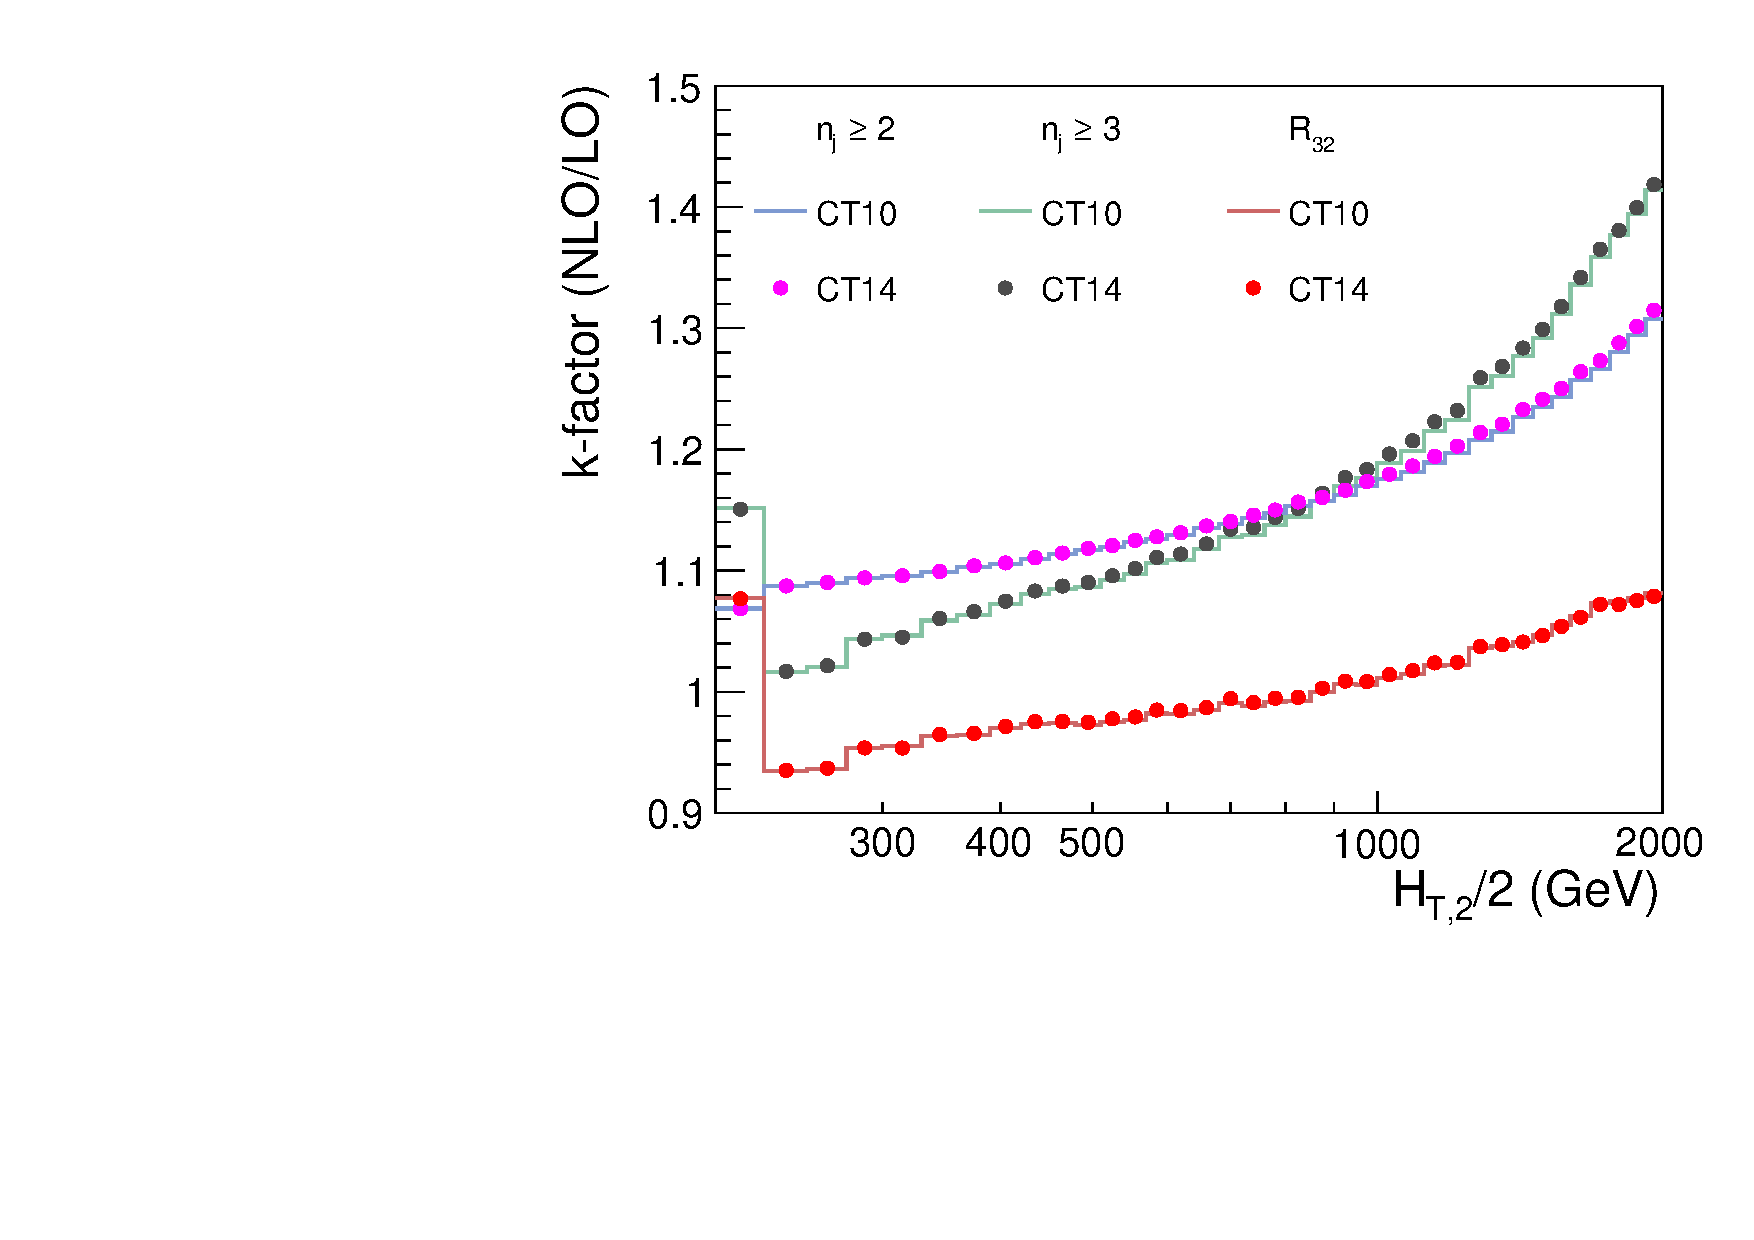
\includegraphics[width=0.51\textwidth]{Plots_HT_2_150/Kfactor_all_1.pdf}%
 ~~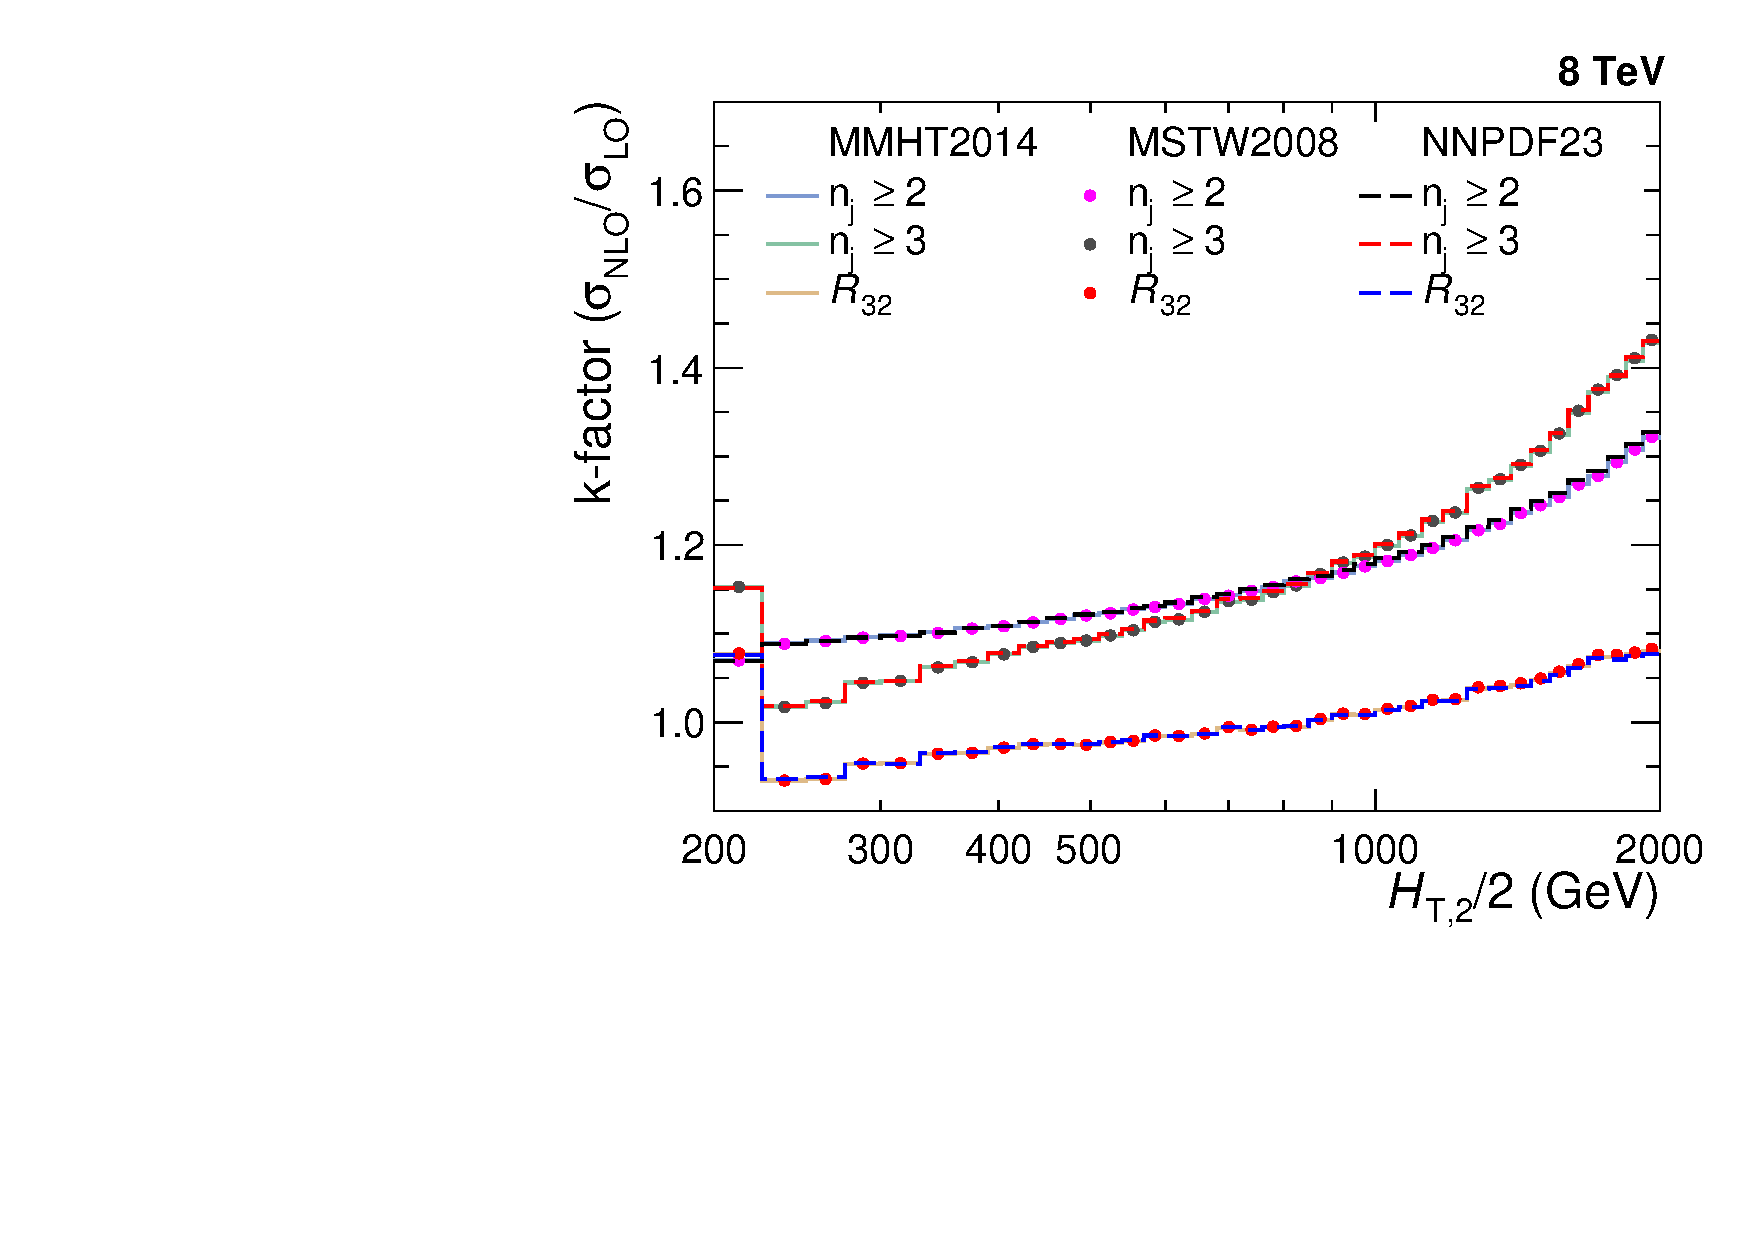
\includegraphics[width=0.51\textwidth]{Plots_HT_2_150/Kfactor_all_2.pdf}
 \caption{The k-factors of the \NLOJETPP calculations, for inclusive 2-jet and 3-jet event cross-sections and their ratio \ratio, using five different PDF sets.}
 \label{fig:kfactor}
 \end{center}
\end{figure}

\subsection{Non-Perturbative Corrections}
\label{sec:NPcorr}

The fixed-order pQCD NLO calculations predict the parton-level cross-section but lacks accuracy due to several effects. The partons which are emitted close to each other in phase space are not handled well in lower order perturbation theories and hence requires a parton shower (PS) correction. The scattering phenomena between partons within a colliding proton, other than the hard scattering, are known as multi-parton interactions (MPI). The partons of the hard scattering forms colorless bound states called hadrons through a process of hadronization (HAD). The MPI and hadronization cannot be modelled well within the perturbative framework. Since the fixed-order NLO calculations do not include these additional soft QCD effects, these calculations cannot be compared directly to unfolded data. So the corrections for non-perturbative effects (NP) should be taken into account in NLO calculations. The ratio of cross-section predicted with a nominal event generation interfaced to the simulation of UE contributions and to the one without hadronization and MPI effects gives the correction factors which are defined as : 

\begin{equation}
  \label{Eq:np}
  C^{\rm NP} = \frac{\sigma^{\rm PS \plusn HAD \plusn MPI}}{\sigma^{\rm PS}}
\end{equation}

In this analysis, the NP effects are estimated by using samples obtained from various MC event generators with a simulation of parton shower and underlying-event (UE) contributions. The leading order (LO), \HERWIGPP~\cite{Bahr:2008pv} with the default tune of version 2.3 and \PYTHIAS~\cite{Sjostrand:2006za} with tune \Ztwostar, and the NLO, \POWHEG~\cite{Nason:2004rx,Frixione:2007vw,Alioli:2010xa}, MC event generators are considered. The matrix-element calculation is performed with \POWHEG interfaced to \PYTHIAE with tune CUETS1~\cite{Khachatryan:2015pea} for the UE simulation. The ratio, defined in Eq.~\ref{Eq:np}, is obtained for each MC generator and is fitted by a power-law function defined in Eq.~\ref{Eq:power}. Since this ratio obtained from different MC generators have large differences, so the average of the envelope, which covers all the differences, is taken as the correction factor which is then applied as bin-by-bin multiplicative factor to the parton-level NLO cross-section. The half of the envelope it is taken as the uncertainty on the NP correction factor. 

\begin{equation}
  \label{Eq:power}
  f(\httwo) = a\cdot\big(\httwo\big)^{b}\texttt{+}~c
\end{equation}

The NP correction factors, $C_{\rm 3\hy jet}^{\rm NP}$ and $C_{\rm 2\hy jet}^{\rm NP}$ are calculated for \njt~and \njth~event cross-sections respectively and then their ratio gives the correction factor for \ratio . These are shown in Fig.~\ref{fig:np_factors} for the inclusive 2-jet (top left) and 3-jet event cross-sections (top right), as well as for cross-section ratio \ratio (bottom). The NP corrections amount to $\sim$ 4\hy 5\% for inclusive 2-jet and 3-jet event cross-sections and $\sim$ 1\% for ratio \ratio, for \httwo $\sim$ 300 GeV and decrease rapidly for increasing \httwo. On comparing the NP correction factors of cross-section ratio with that for individual cross-sections, it has been observed that the non-perturbative effects get reduced in the cross-section ratio.

\begin{figure}[!ht]
 \begin{center}
 \hspace*{-5mm}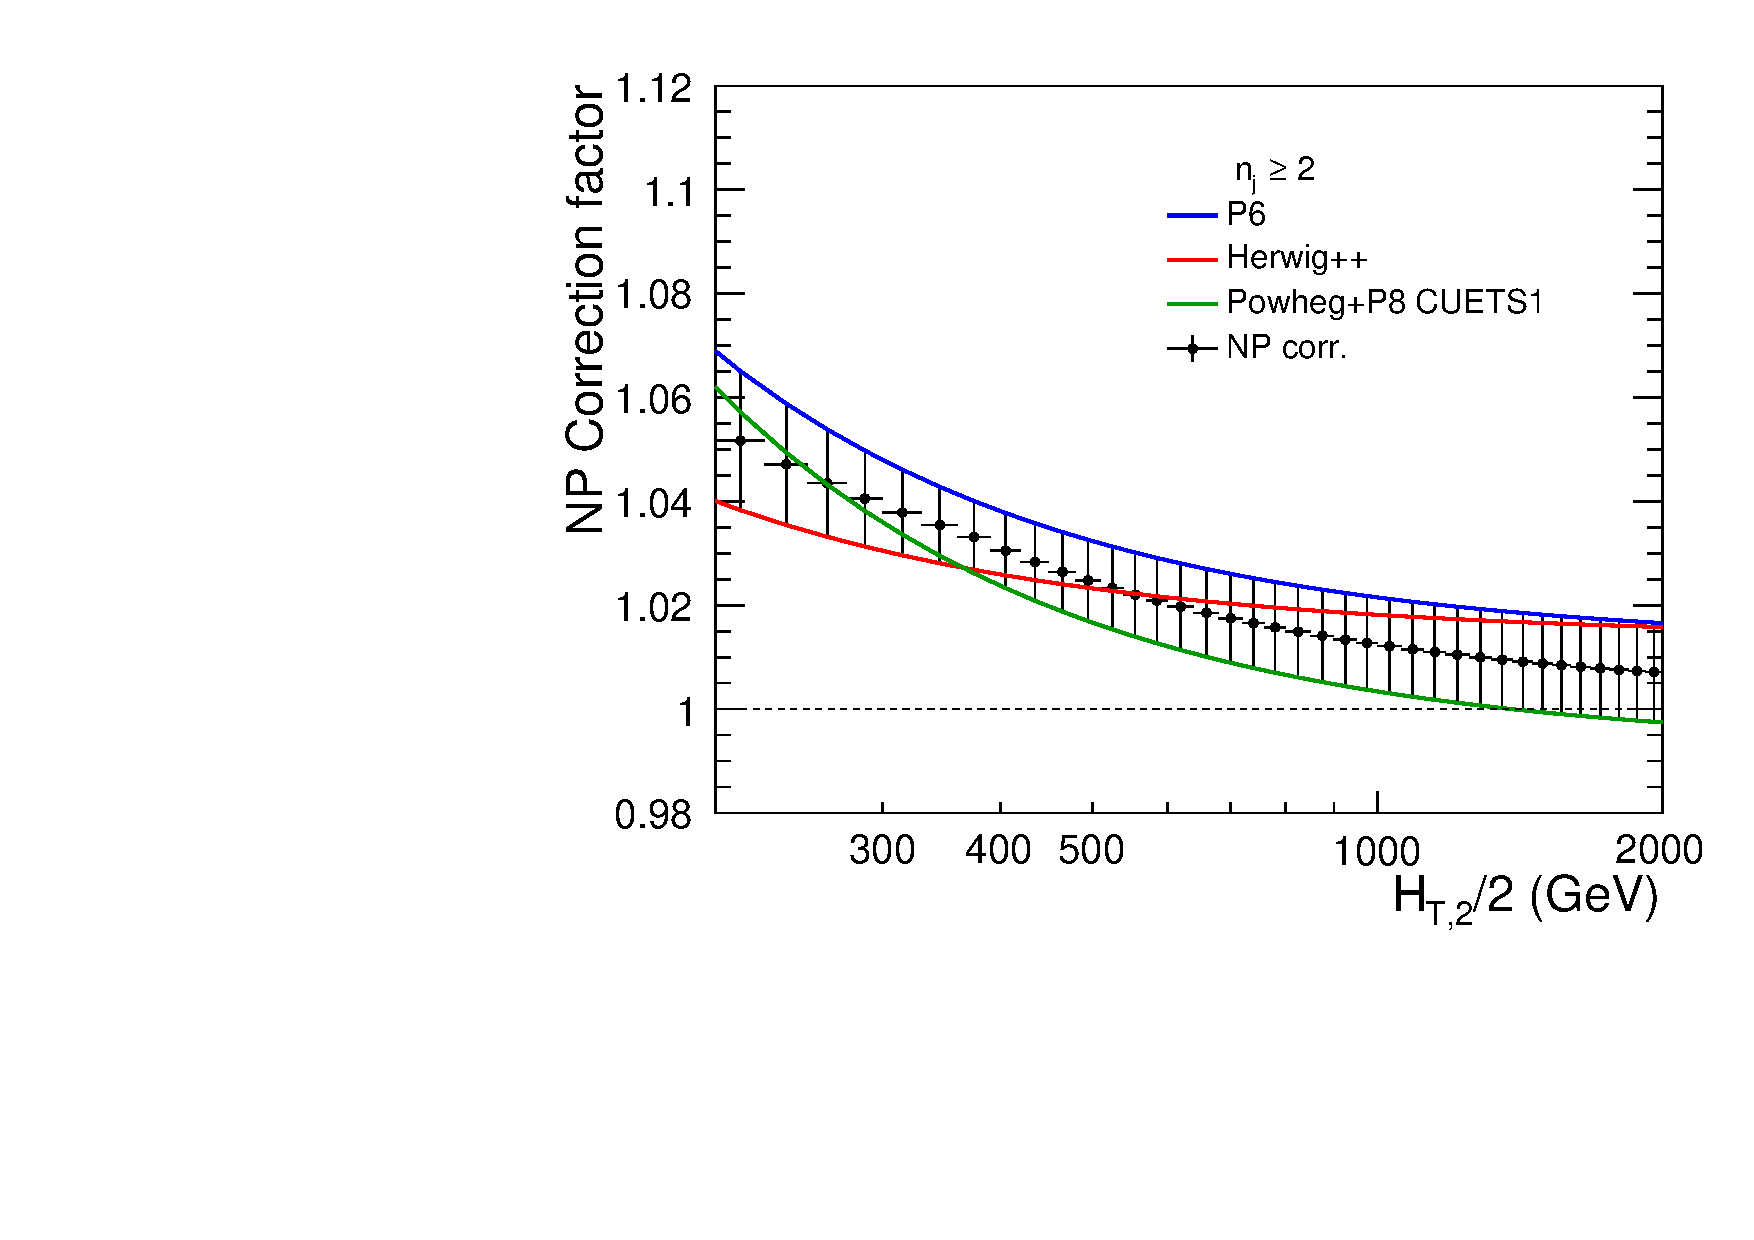
\includegraphics[width=0.51\textwidth]{Plots_HT_2_150/Final_NP_Corr_2.pdf}%
 ~~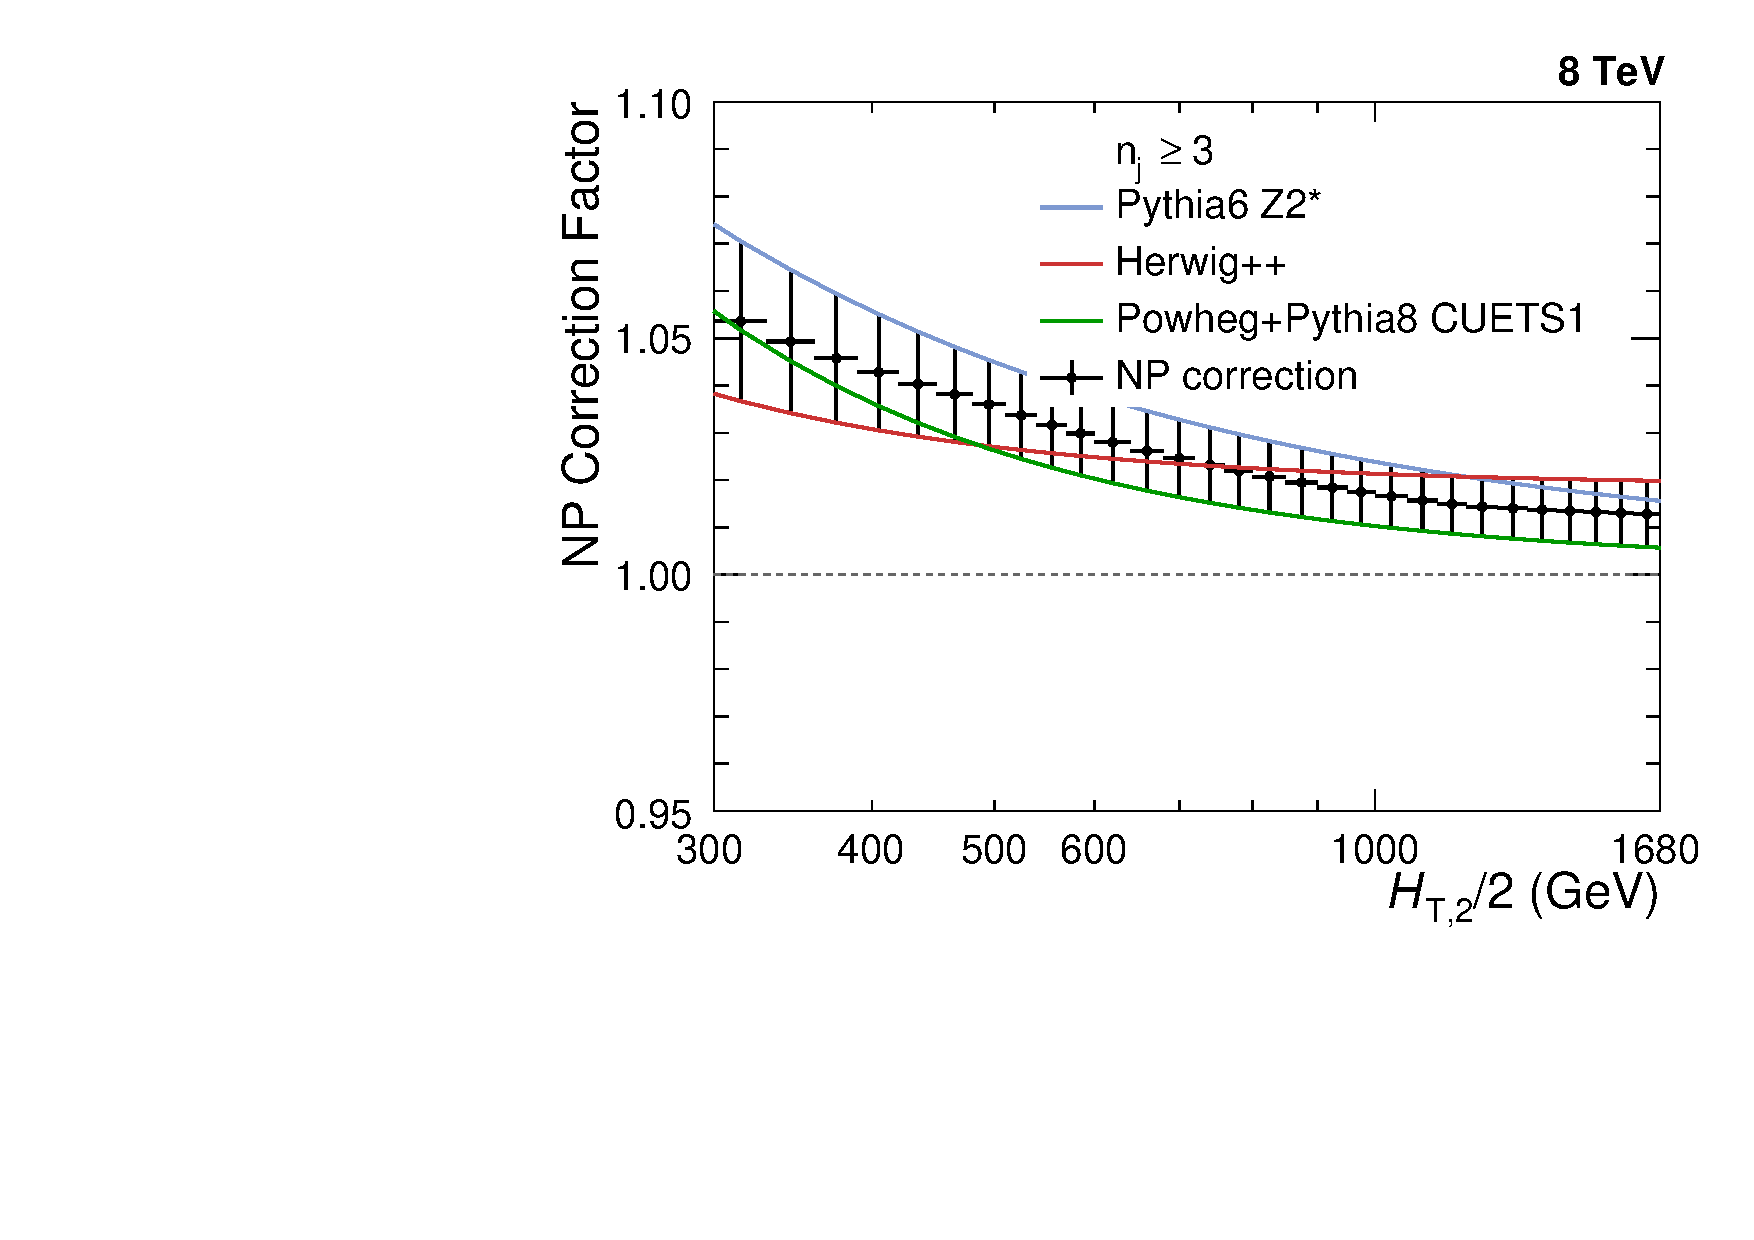
\includegraphics[width=0.51\textwidth]{Plots_HT_2_150/Final_NP_Corr_3.pdf}\\
 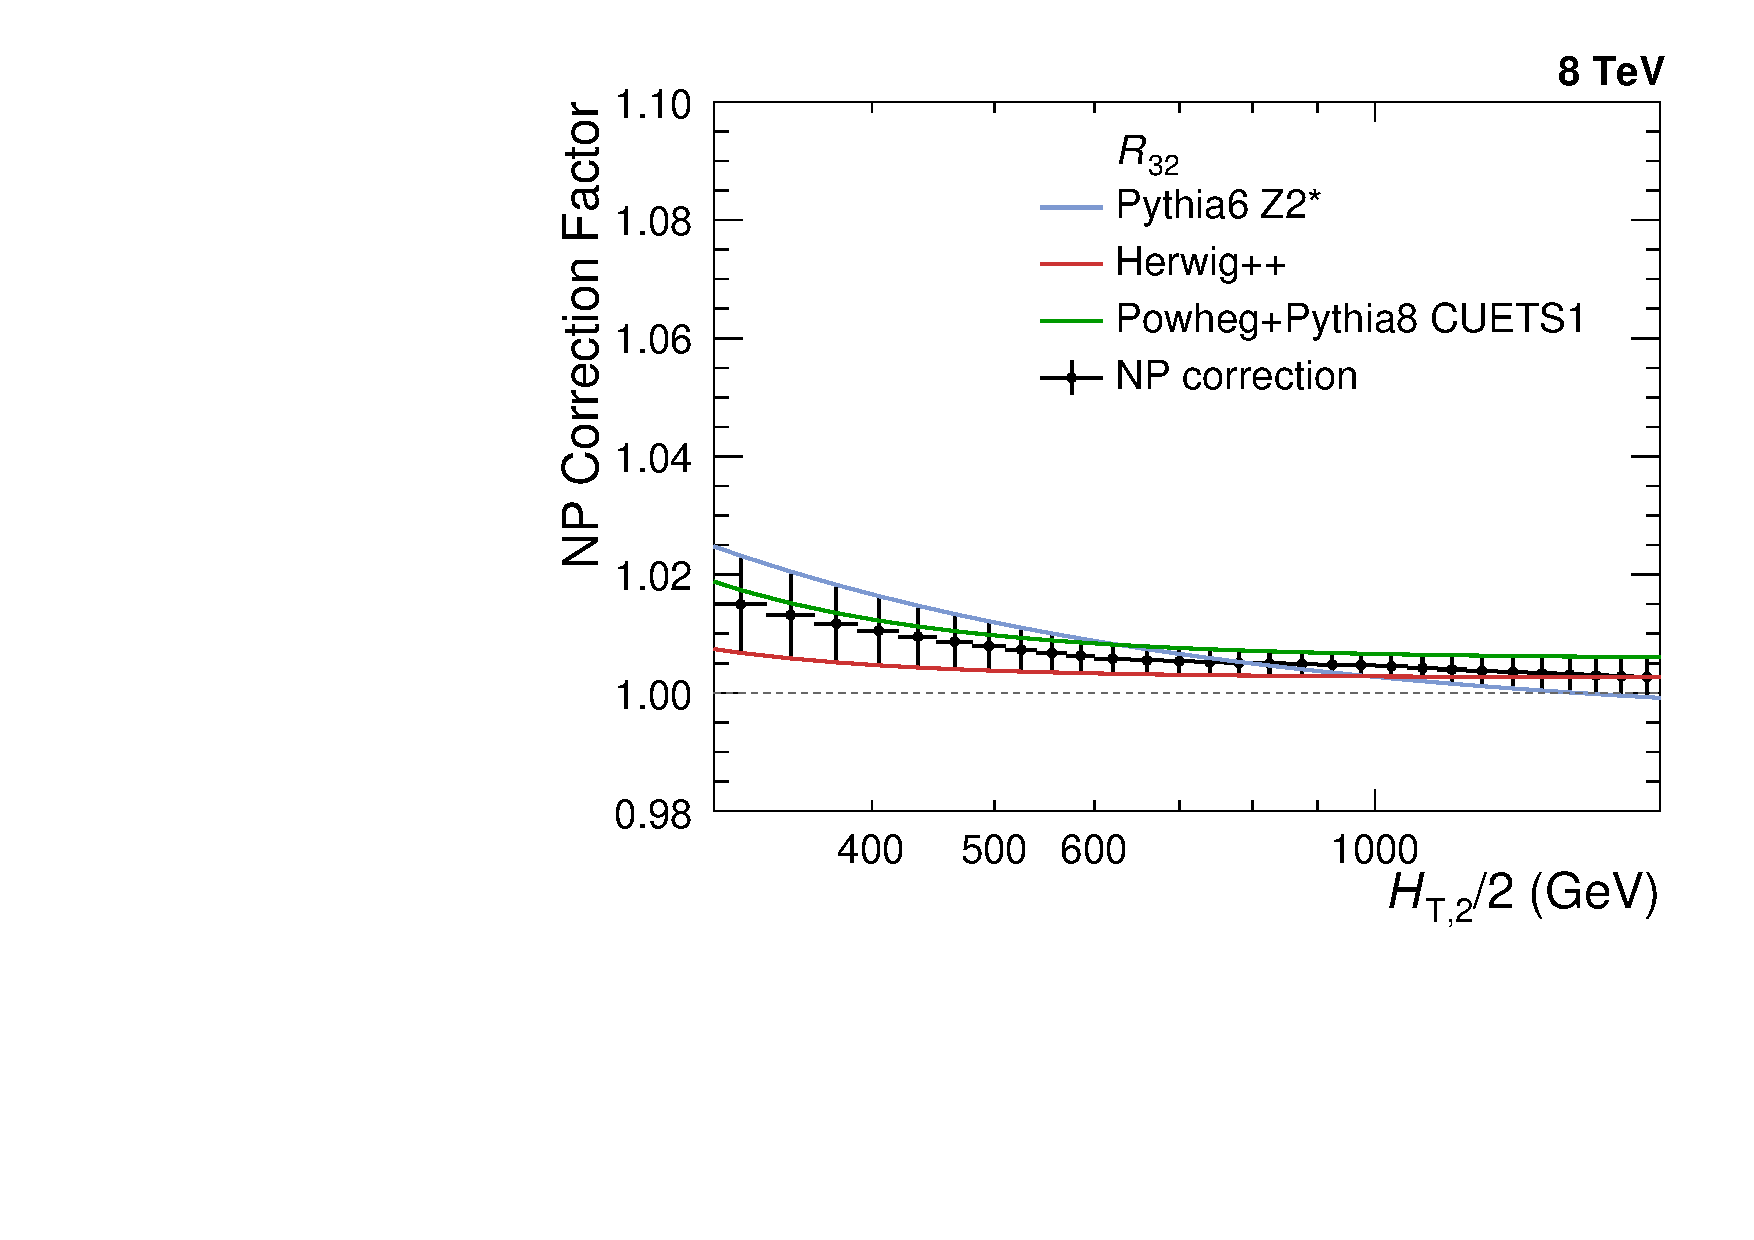
\includegraphics[width=0.51\textwidth]{Plots_HT_2_150/Final_NP_Corr_Ratio_32.pdf}
 \caption{The nonperturbative (NP) corrections are presented as a function of \httwo for inclusive 2-jet (top left) and 3-jet (top right) event cross-sections, as well as their ratio \ratio. These corrections are calculated from the leading order \HERWIGPP with the default tune of version 2.3 (red line) and \PYTHIAS with tune \Ztwostar (blue line); and the next-to-leading order \POWHEG interfaced to \PYTHIAE with tune CUETS1 (green line) Monte Carlo event generators. The black solid circles give the average NP correction factor along with the uncertainty shown by the error bars. }
 \label{fig:np_factors}
 \end{center}
\end{figure}
%This is because the strong coupling constant, \alpsns, decreases with increasing energy faster than the EW one as ${\rm \alpha_{W} \equiv \alpha_{EM}/sin^2 \theta_W}$ (where  $\alpha_{EM}$ is the electro,agnetic (EM) coupling constant and ${\rm \theta_W}$ is the weak angle). Also the purely weak part of higher order EWeffects produces lead-ing corrections of the typeαWlog(μ2/M2W), whereinμrepresents some typical energy scaleaffecting the hard process in a given observable, e.g., the partonic CM energy√ˆ. The

\subsection{Electroweak Corrections}
\label{sec:EW}
In LHC, the centre-of-mass energy of proton-proton collisions is well beyond the electroweak (EW) scale $\sim$O(100 GeV). At such a high energy, the impact of higher order EW corrections is much more with respect to QCD effects \cite{Hollik:2004dz} and affect jet cross-sections at large jet \pt. The quark-quark scattering processes involving virtual exchanges of massive W and Z bosons contribute to electroweak (EW) corrections. The fixed-order QCD calculations do not include EW corrections and hence the NLO theory calculations are corrected for EW effects. The EW corrections have been calculated for inclusive 1-jet and 2-jet case, in Ref. \cite{Dittmaier:2012kx}. The EW correction factors in the phase space of the measurement are shown as a function of \httwo in Fig.~\ref{fig:EW} for inclusive 2-jet event cross-sections. These correction factor increases up to 13\% at high ends of \httwo which are applied as a bin-by-bin correction factor to the fixed-order calculation of \NLOJETPP. To see the effects of EW corrections, a ratio of data to theory predictions obtained using CT10-NLO PDF set and corrected with NP effects without including EW corrections (left) and including EW corrections (right) is plotted for inclusive 2-jet event cross-sections in Fig.~\ref{fig:EW_Comp}. On comparing both the figures, it is observed that the EW corrections significantly improve the agreement between data and prediction in the high \httwo region. EW corrections are not available yet for inclusive 3-jet production and hence not applied for inclusive 3-jet event cross-sections. The guess from theory side is that EW for inclusive 2-jet and 3-jet will be similar, so for \ratio, it is assumed to be equal to the factor of 1. Since the EW effects are not taken care of in MC simulations so these corrections are applied to MC predictions also. 

\begin{figure}[!t]
 \begin{center}
 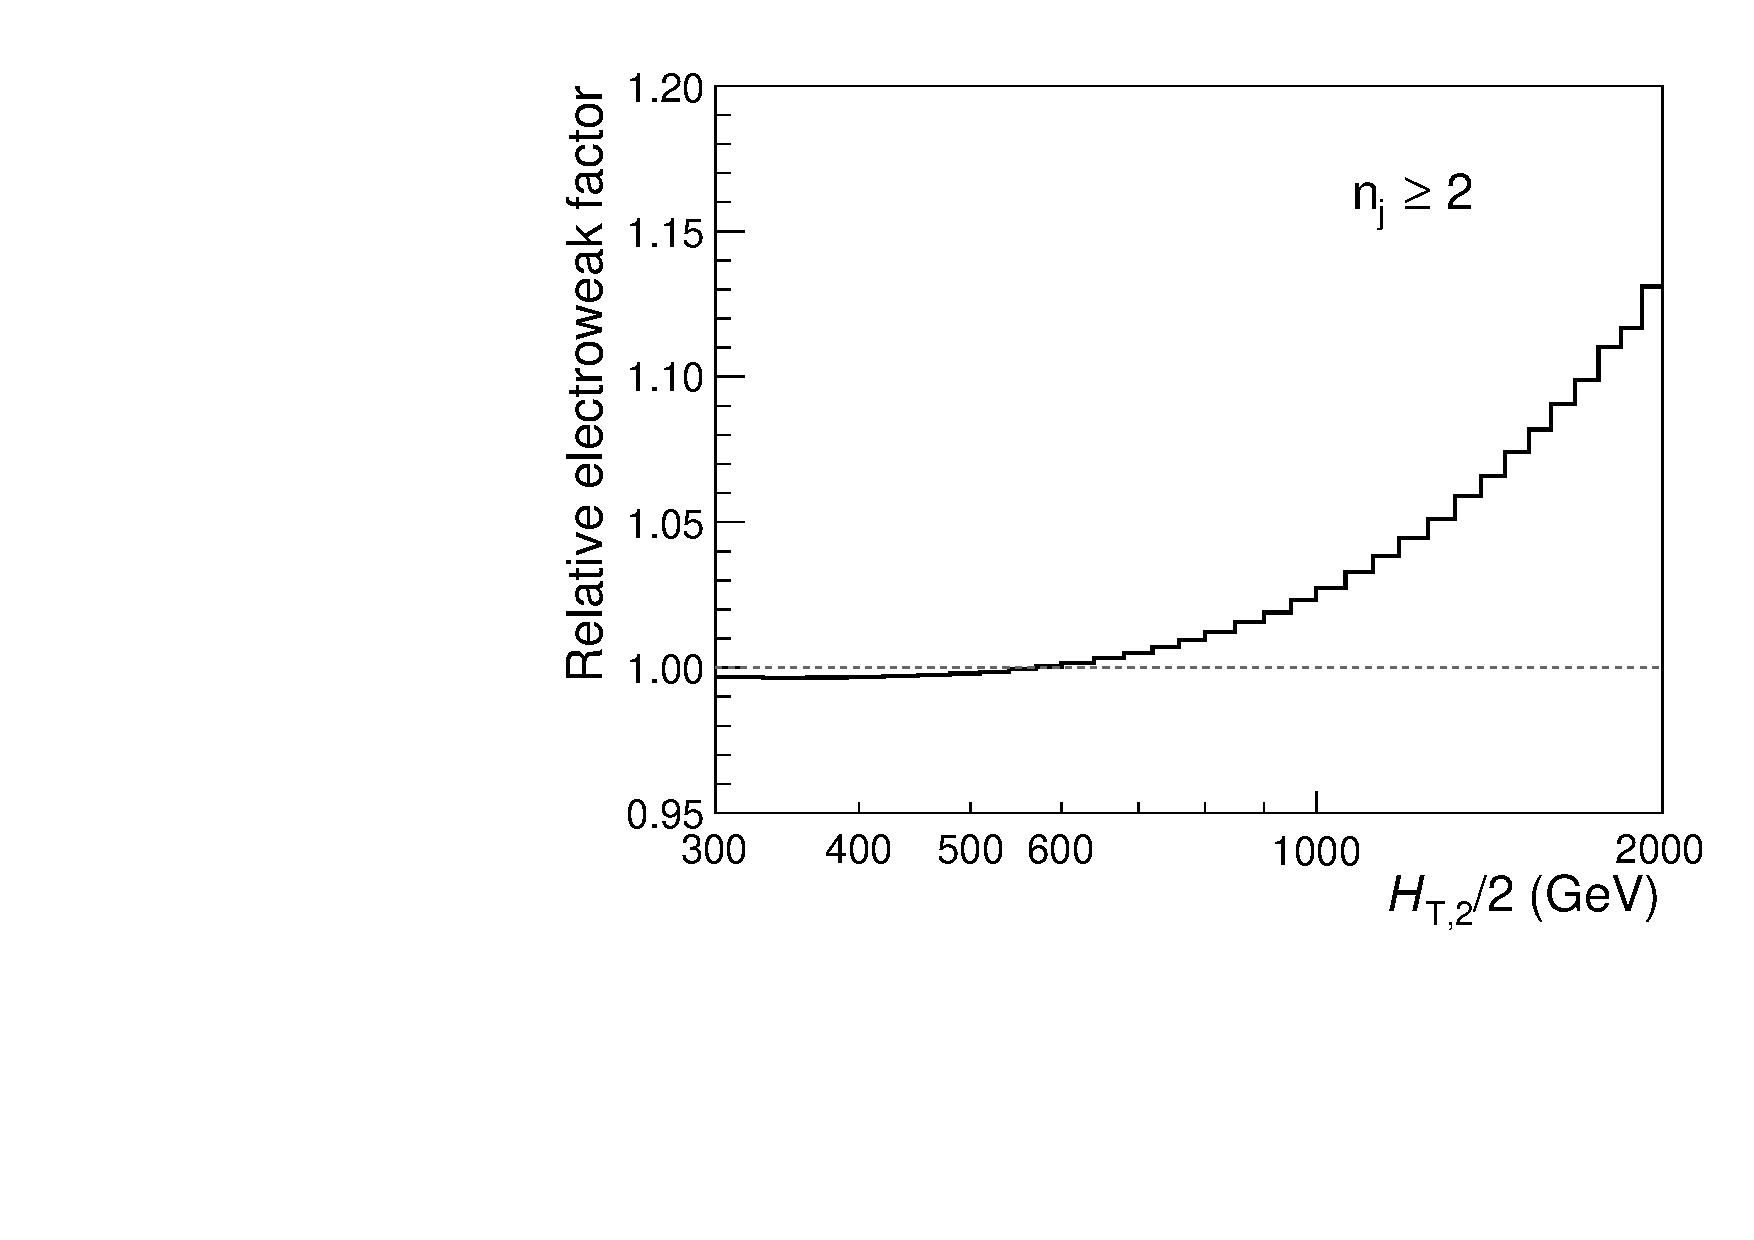
\includegraphics[width=0.51\textwidth]{Plots_HT_2_150/EW_2.pdf}
 \caption{The electroweak (EW) corrections \cite{Dittmaier:2012kx} in the phase space of the measurement are shown as a function of \httwo for inclusive 2-jet event cross-sections. These corrections are applied as a bin-by-bin correction factor to the fixed-order calculation of \NLOJETPP as well as the MC predictions of \MadGraphFn\plusn \PYTHIAS. The EW correction factor increases up to 13\% at high ends of \httwo and significantly improves the agreement between data and prediction.}
 \label{fig:EW}
 \end{center}
\end{figure}

\begin{figure}[!h]
 \begin{center}
 \hspace*{-5mm}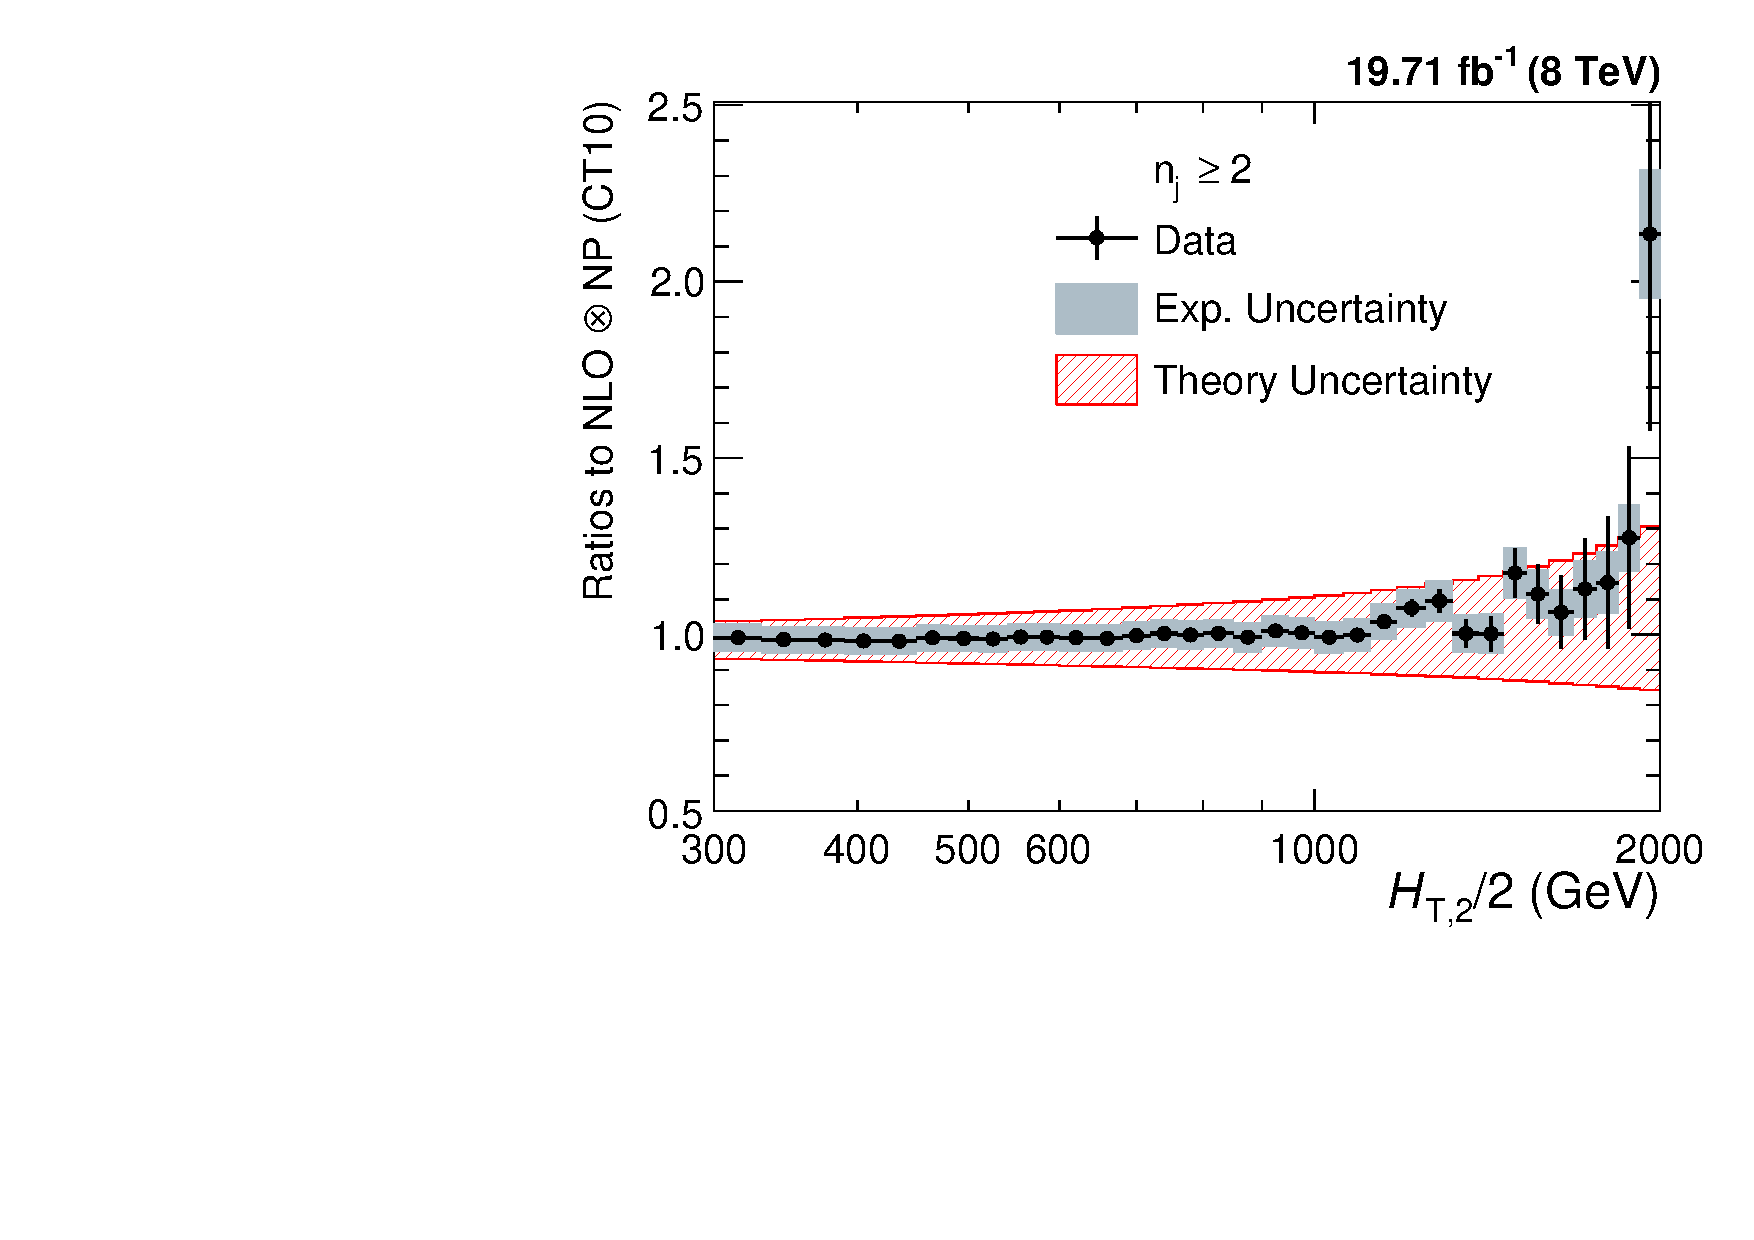
\includegraphics[width=0.5\textwidth]{Plots_HT_2_150/Comparison_data_NLO_2_NoEW.pdf}
 ~~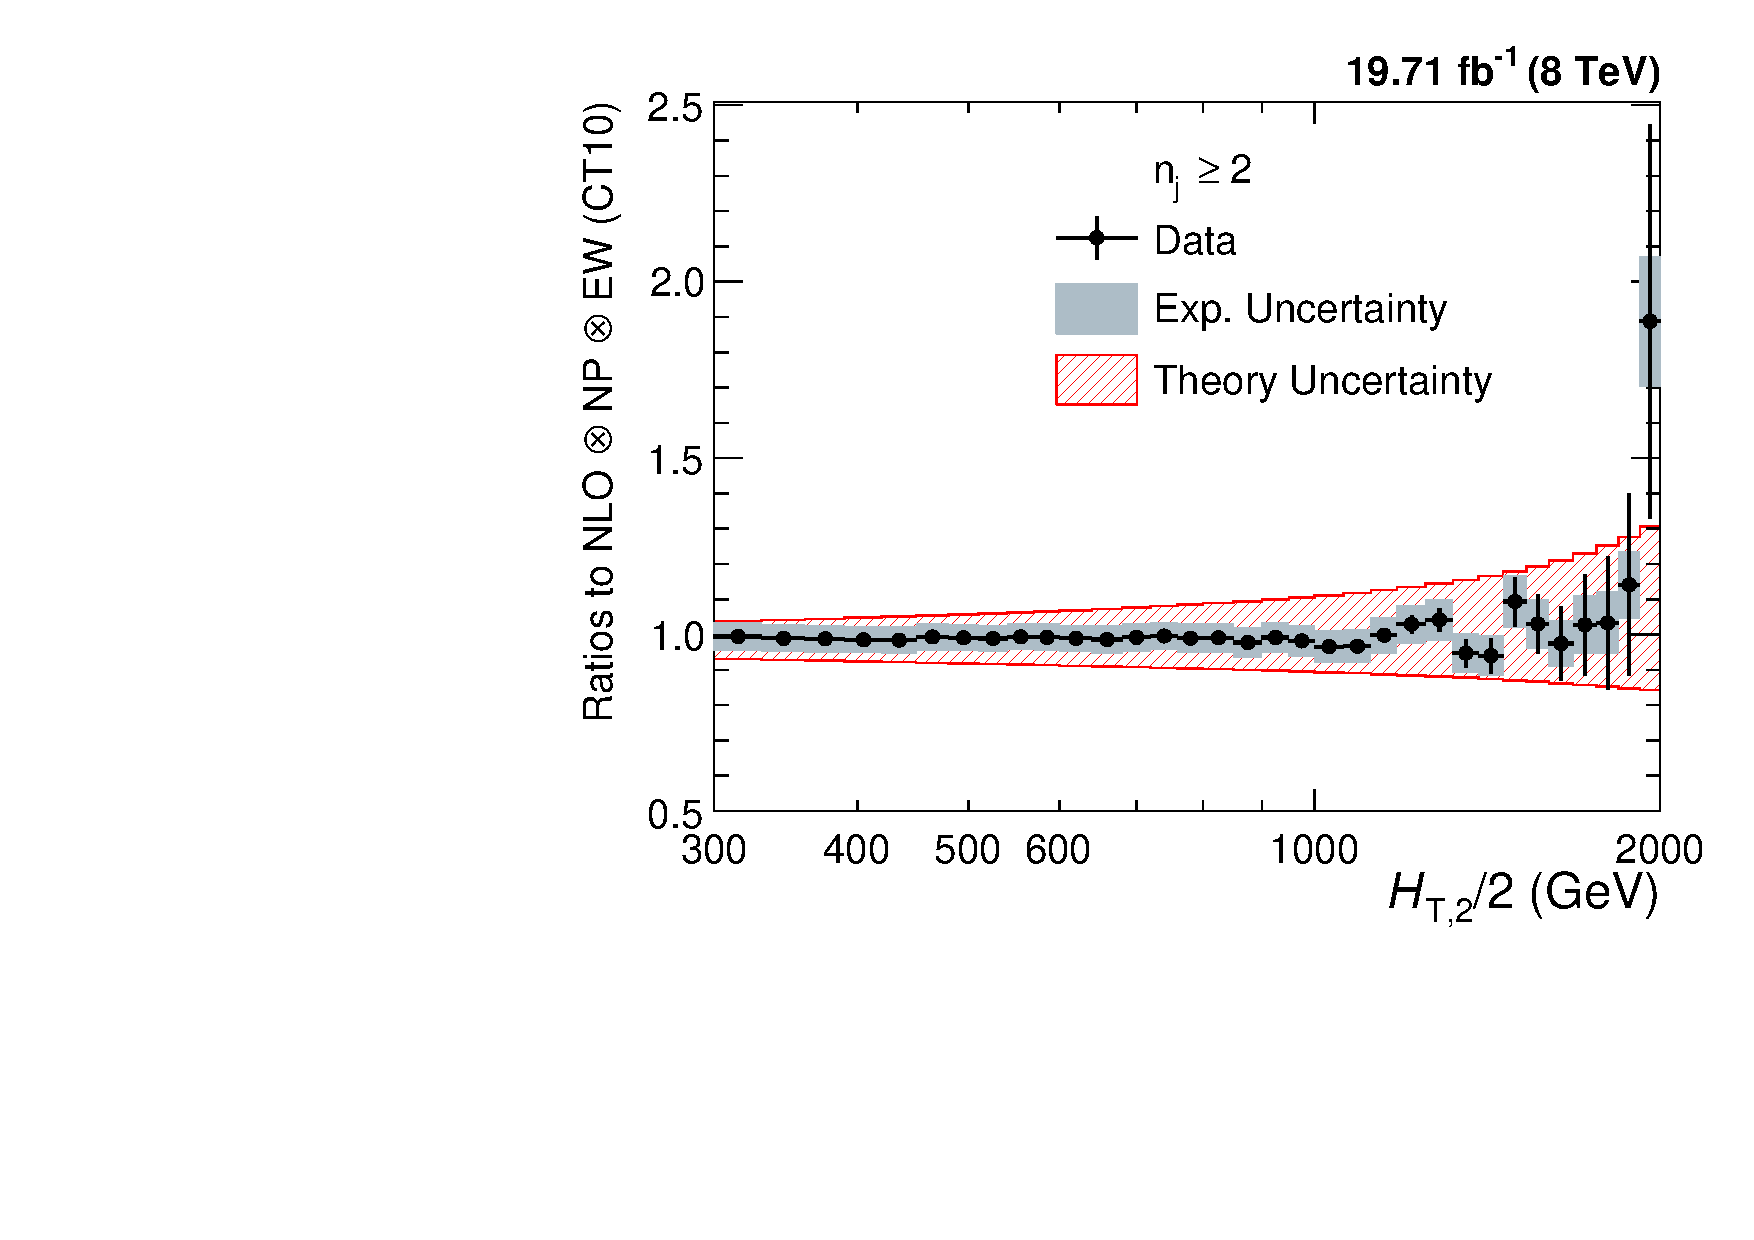
\includegraphics[width=0.5\textwidth]{Plots_HT_2_150/Comparison_data_NLO_2_EW.pdf}
 \caption{Ratio of data over theory obtained using the CT10-NLO PDF set and corrected with non-perturbative effects (NP) without including electroweak (EW) corrections (left) and including EW corrections (right) is shown for inclusive 2-jet event cross-sections. The error bars represents the statistical uncertainty of the data and the shaded rectangles represents the total experimental systematic uncertainty. The shaded band around unity indicate the total uncertainty of the theory. The EW corrections significantly improve the agreement between data and prediction in the high \httwo region.}
 \label{fig:EW_Comp}
 \end{center}
\end{figure}

\section{Theoretical Uncertainties}
\label{sec:theory_unc}
The measurements are not only sensitive to experimental uncertainties but also to the theoretical uncertainties. The renormalization  and  factorization scale variations, PDF uncertainties and the non-perturbative corrections contribute to theoretical uncertainties which are described below : 

\subsection{Scale Uncertainty}
\label{sec:scale_unc}
In perturbative QCD calculations of cross-sections, one has to choose a renormalization (\mur) and factorization (\muf) scale. The dependence on scales is negligible if these calculations are performed for all orders of the perturbative series. But the perturbative series is truncated at NLO, so there is a scale dependence of the measurement which is covered by systematic uncertainty known as scale uncertainty. The scale uncertainty is evaluated with the conventional recipe of varying the default scale \httwo chosen for \mur and \muf independently in the following six combinations: (\mur/\httwo, \muf/\httwo) = (1/2,1/2), (1/2,1), (1,1/2), (1,2), (2,1) and (2,2). The maximal upwards and downwards deviations in cross-section from the central prediction give the scale uncertainty. To calculate the scale uncertainty for cross-section ratio \ratio, first \ratio is obtained for each above mentioned scale choice and then its difference from central \ratio is taken. The scale uncertainty calculated using CT10-NLO PDF set ranges for inclusive 2-jet events from 5\% to 13\%, for inclusive 3-jet events from 11\% to 17\% and for \ratio from 6\% to 8\%.

\subsection{PDF Uncertainty}
\label{sec:pdf_unc}
The calculation of jet cross-sections in proton-proton collisions relies upon the knowledge of parton distribution functions (PDF). These PDF sets are determined by global fits to all the available deep inelastic scattering (DIS) and related hard scattering data from different experiments. The various sources affect the PDFs such as theory model, input parameters like the strong coupling constant \alpsns, the quark masses and the statistical and systematic uncertainty sources of the data included in the PDF fit. These sources contribute to PDF uncertainty which is evaluated according to the prescriptions given for each PDF set. The CT10-NLO PDF set \cite{Lai:2010vv,Pumplin:2002vw} employ the eigenvector method to evaluate the PDF uncertainties. The CT10-PDF set consists of $N_\mathrm{ev}=26$ eigenvectors with two PDF members per eigenvector $k$, which are varied upwards and downwards to generate a set of eigenvector pairs. The asymmetric uncertainties, $\Delta X^{+}$ and $\Delta X^{-}$, of a quantity X are given by Eq.~\ref{eq:unc_pdf} where $X_0$ is the central prediction, $X^{+}_k$ and $X^{-}_k$ are the predictions using the upwards and downwards variation of each eigenvector $k$. 

\begin{equation}
\label{eq:unc_pdf}
\begin{gathered}
\Delta X^+ =  \sqrt{\sum \limits_{k=1}^{N_\mathrm{ev}}\big[{\rm max}(X^{+}_{k}-X^{0},X^{-}_{k}-X^{0},0)\big]^2} \\
\Delta X^- =  \sqrt{\sum \limits_{k=1}^{N_\mathrm{ev}}\big[{\rm min}(X^{+}_{k}-X^{0},X^{-}_{k}-X^{0},0)\big]^2}
\end{gathered}
\end{equation}

The symmetric uncertainty ($\Delta X^{\pm}$) is given by half the difference of the upwards and downwards variations :

\begin{equation}
\label{eq:unc_pdf_symm}
\Delta X^{\pm} = \sqrt{\sum \limits_{k=1}^{N_\mathrm{ev}} \Bigg[\frac{X^{+}_{k}-X^{-}_{k}}{2}\Bigg]^2}
\end{equation}

The CT10-NLO PDF set uncertainties are downscaled by a factor of 1.64 in order to have the uncertainties at the 68.3\% confidence level CL(1$\sigma$) instead of 90\% CL(2$\sigma$) such that to have a uniform treatment with respect to other PDF sets. The PDF uncertainty as derived with the CT10-NLO PDF set is the dominant source of uncertainty and ranges from 3\% to 30\% for inclusive 2-jet and from 4\% to 32\% for 3-jet cross-sections. For \ratio, the ratio of predictions for inclusive 3-jet to that of 2-jet is taken for each eigen vector with upwards and downwards variations separately and then PDF uncertainty is calculated as done for individual cross-sections. The PDF uncertainty ranges and from 2\% to 10\% for cross-section ratio \ratio. 

\subsection{Non-perturbative Uncertainty}
As discussed in \ref{sec:NPcorr}, the differences in the non-perturbative (NP) corrections calculated from various Monte Carlo event generators introduce the NP uncertainty which is of the order of 1\% and 1 to 2\% for inclusive 2-jet and 3-jet event cross-sections respectively, and \ls 1\% for cross-section ratio \ratio.

\begin{figure}[!h]
 \begin{center}
 \hspace*{-5mm}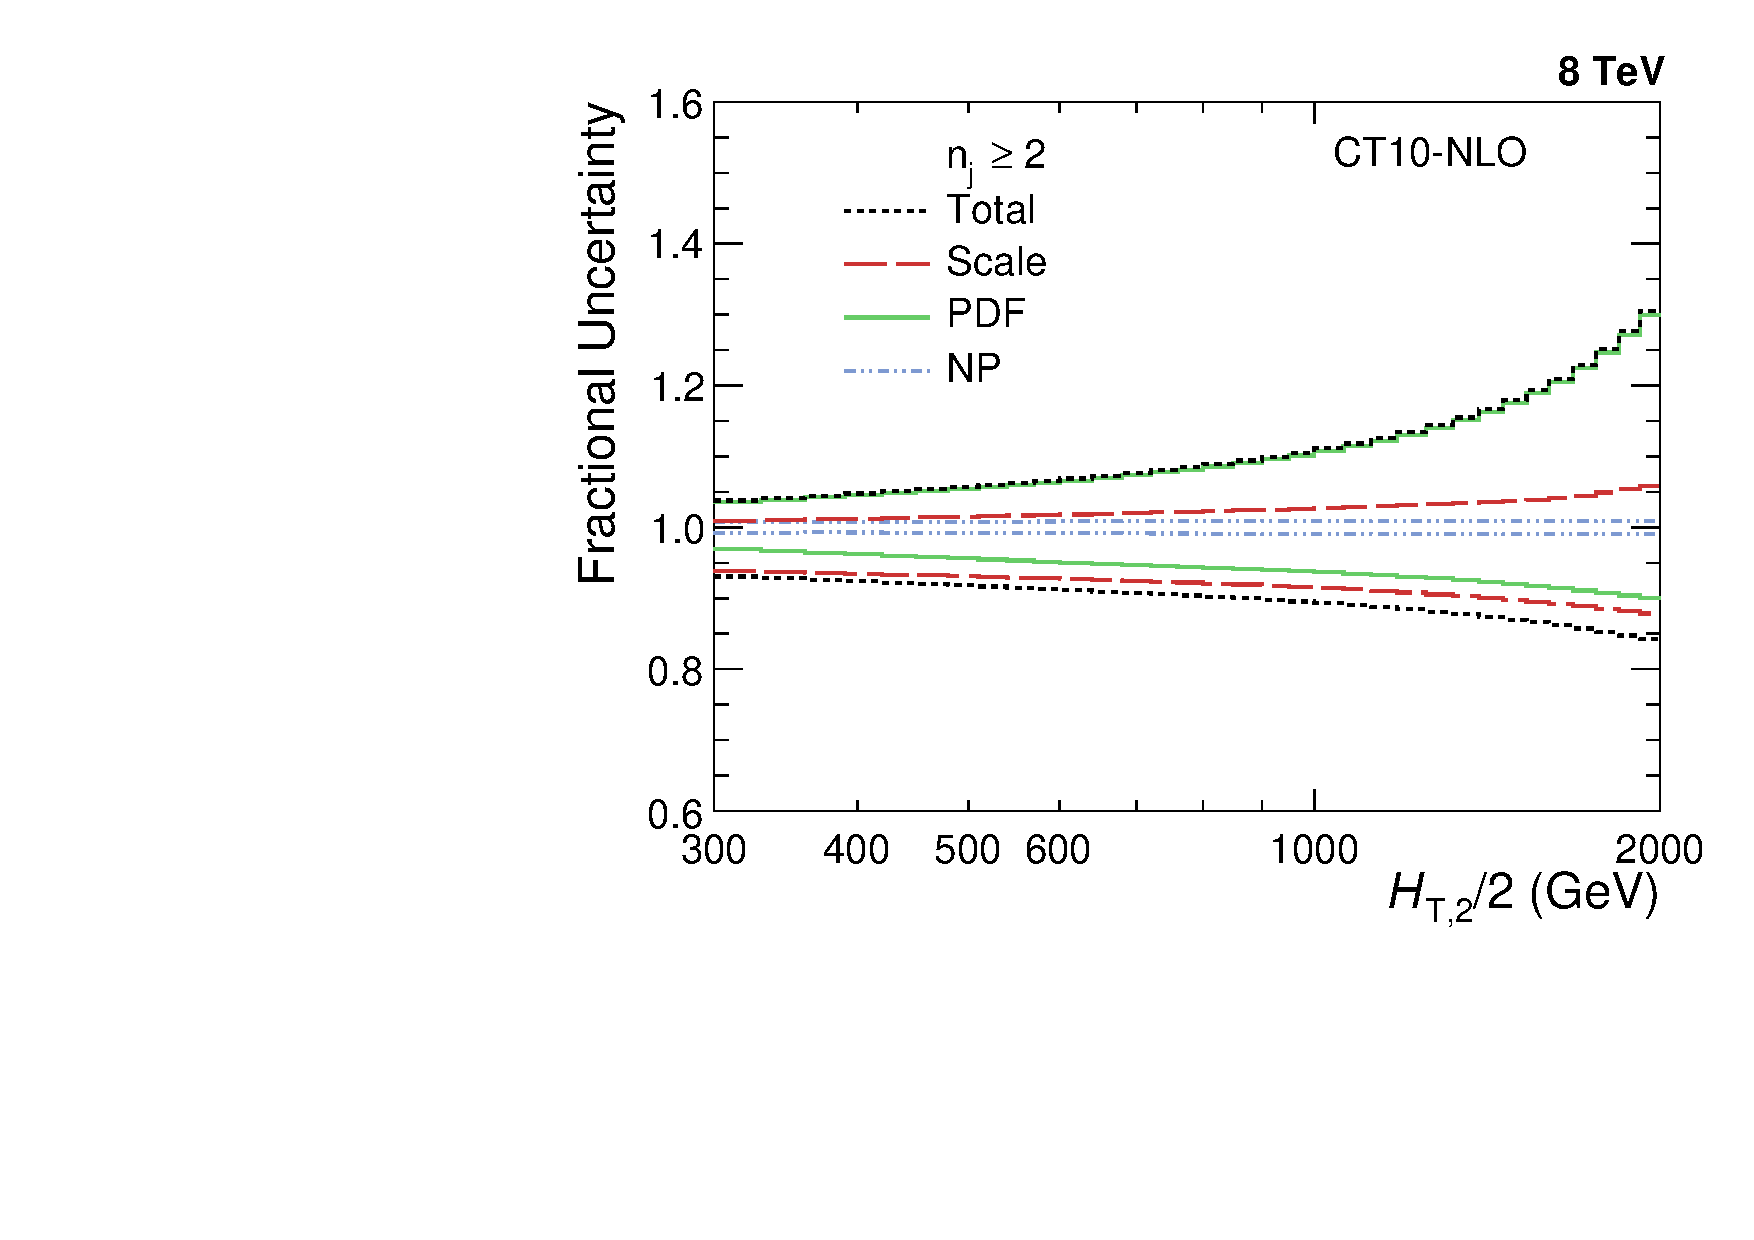
\includegraphics[width=0.51\textwidth]{Plots_HT_2_150/Theory_Unc_2.pdf}%
 ~~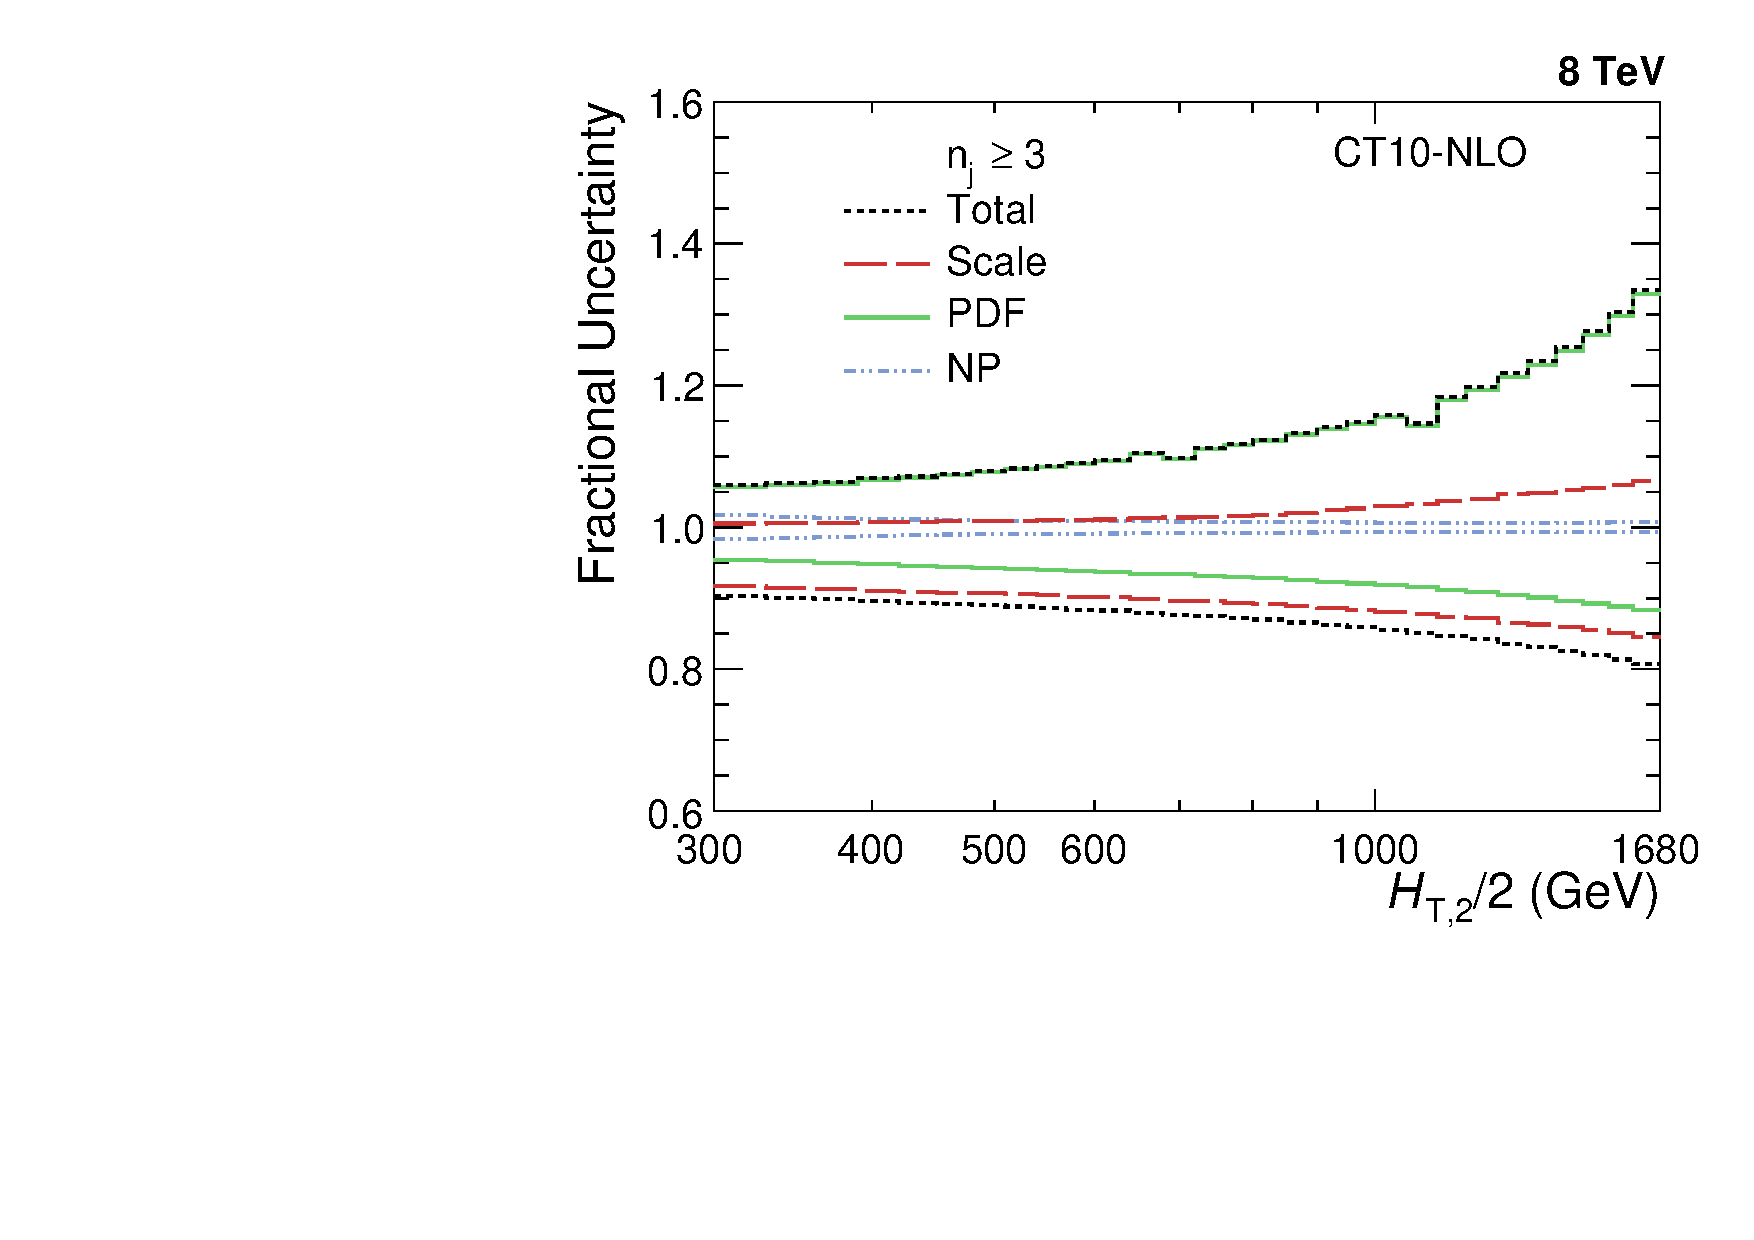
\includegraphics[width=0.51\textwidth]{Plots_HT_2_150/Theory_Unc_3.pdf}\\
 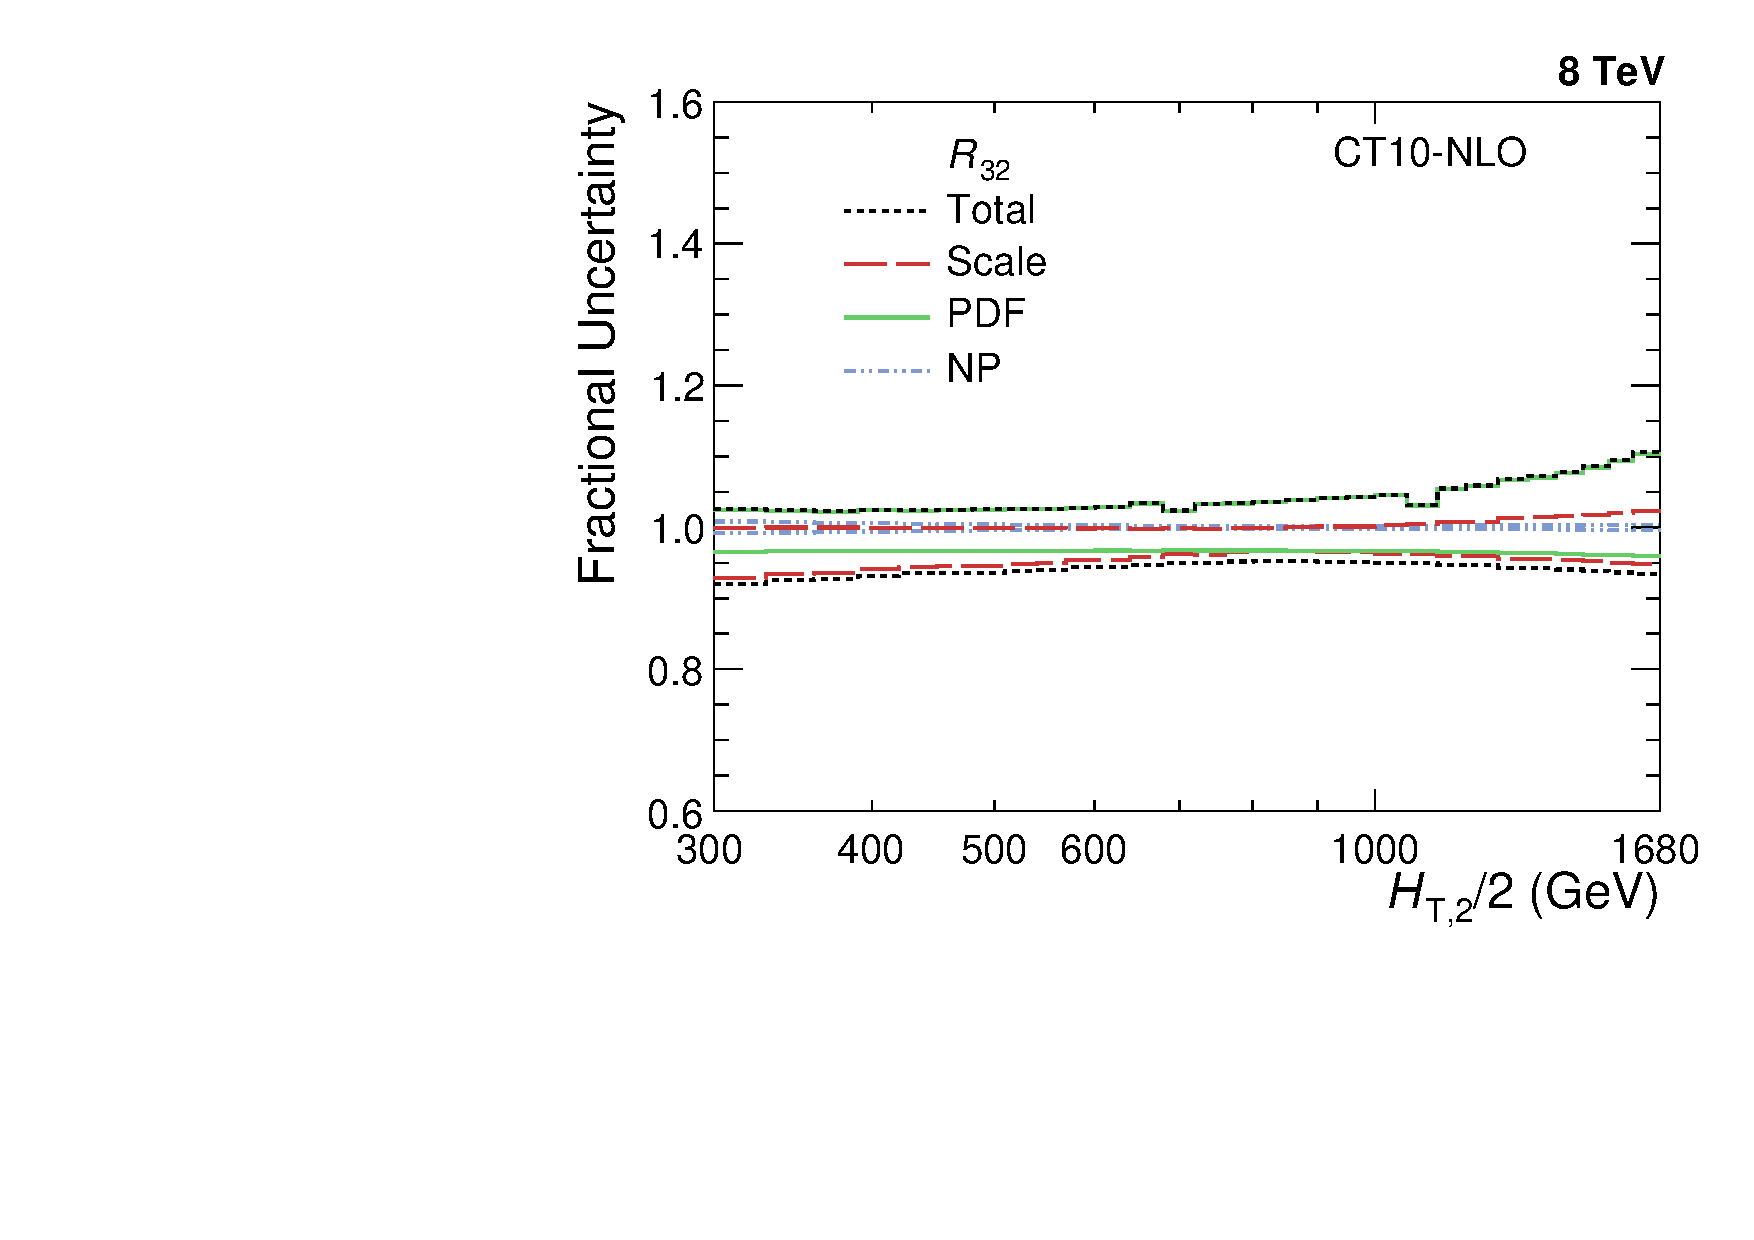
\includegraphics[width=0.51\textwidth]{Plots_HT_2_150/Theory_Unc_Ratio_32.pdf}\\  
 \caption{The systematic theoretical uncertainties affecting the cross-section measurement for inclusive 2-jet (top left) and 3-jet events (top right) and their ratio \ratio (bottom). The scale (red dashed line), PDF (green line) and NP (blue dashed line) uncertainties as well as total uncertainty (black dashed line) obtained using CT10-NLO PDF set are shown. The total theoretical uncertainty is asymmetric and is dominated by PDF uncertainty.}
 \label{fig:theory_unc}
 \end{center}
\end{figure}

\subsection{Total Theoretical Uncertainty}
The total systematic theoretical uncertainties are obtained as the quadratic sum of the scale, PDF and NP uncertainties. Figure~\ref{fig:theory_unc} presents the systematic theoretical uncertainties affecting the cross-section measurement for inclusive 2-jet (top left) and 3-jet events (top right) and the cross-section ratio \ratio (bottom), using CT10-NLO PDF set. The scale (red dashed line), PDF (green line) and NP (blue dashed line) uncertainties as well as total theoretical uncertainty (black dashed line) are shown. The total theoretical uncertainty is asymmetric and is dominated by PDF uncertainty which grows in magnitude with increasing value of \httwo. Table~\ref{tab:theory_unc} quotes the values of the theoretical uncertainty from each source as well as total uncertainty affecting the measurements. The bin-wise values of uncertainties (in \%) from each source as well as total uncertainty are shown in Tables~\ref{tab:exp_unc2_th},~\ref{tab:exp_unc3_th} and~\ref{tab:exp_unc_ratio_th} for \njt~and \njth~event cross-sections and cross-section ratio \ratio, respectively. The computation of the NLO predictions with \NLOJETPP is also subject to statistical fluctuations from the complex numerical integrations. For the inclusive 2-jet event cross-sections this uncertainty is smaller than about a per mille, while for the inclusive 3-jet event cross-section it amounts to 1-9 per mille. Hence the statistical uncertainty is not considered in the total theoretical uncertainty. The small dips at $\sim$700 and 1000 GeV in the PDF uncertainty for inclusive 3-jet events cross-sections and cross-section ratio \ratio is a feature of the CT10-NLO PDF set.
 
\begin{table}[!h]
%\centering
  \caption{Overview of all systematic theoretical uncertainties, obtained using CT10-NLO PDF set, affecting the measurement of cross-sections for inclusive 2-jet (left) and inclusive 3-jet events (middle) and cross-section ratio \ratio (right).}
  \label{tab:theory_unc}
  \vspace{2mm}
  \begin{tabular}{lccc}
  \hline\hline
  {\bf Uncertainty Source}& {\bf Inclusive 2-jet} & {\bf Inclusive 3-jet} & {\bf \ratio} \rbthm\\ \hline
  Scale                   & 5 to 13\%             & 11 to 17\%            & 6 to 8\%  \rbtrr\\
  PDF                     & 3 to 30\%             & 4 to 32\%             & 2 to 10\% \rbtrr\\
  Non-perturbative (NP)   & 1\%                   & 1 to 2\%              & $<$ 1\%   \rbtrr\\\hline
  Total                   & 3 to 30\%             & 5 to 34\%             & 3 to 11\% \rbtrr\\
  \hline\hline
  \end{tabular}
\end{table}

\section{Comparison of Theory to Data}
After correcting the measurement for detector effects as well as NLO pQCD calculations for non-perturbative (NP) and electroweak (EW) effects, it is now possible to compare the measured cross-sections with the theory predictions. Figure~\ref{fig:data_NL0_MC} shows the measured differential inclusive 2-jet and 3-jet event cross-sections as a function of \httwo after unfolding for detector effects. On the left, the measurements (points) are compared to the \NLOJETPP predictions using the CT10-NLO PDF set (line), corrected for NP effects and in addition for EW effects in the 2-jet case. On the right, the comparison is made to the predictions from \MadGraphFn \plusn \PYTHIAS (MG\plusn P6) with tune \Ztwostar (line), corrected for EW effects in the 2-jet case. The error bars give the total experimental uncertainty, given by the quadrature sum of the statistical and systematic uncertainties. On a logarithmic scale, the data are in well agreement with the NLO predictions over the whole range of \httwo from 300 GeV up to 2000 (2-jet) and 1680 GeV (3-jet) respectively. 

\begin{figure}[!h]
 \hspace*{-5mm}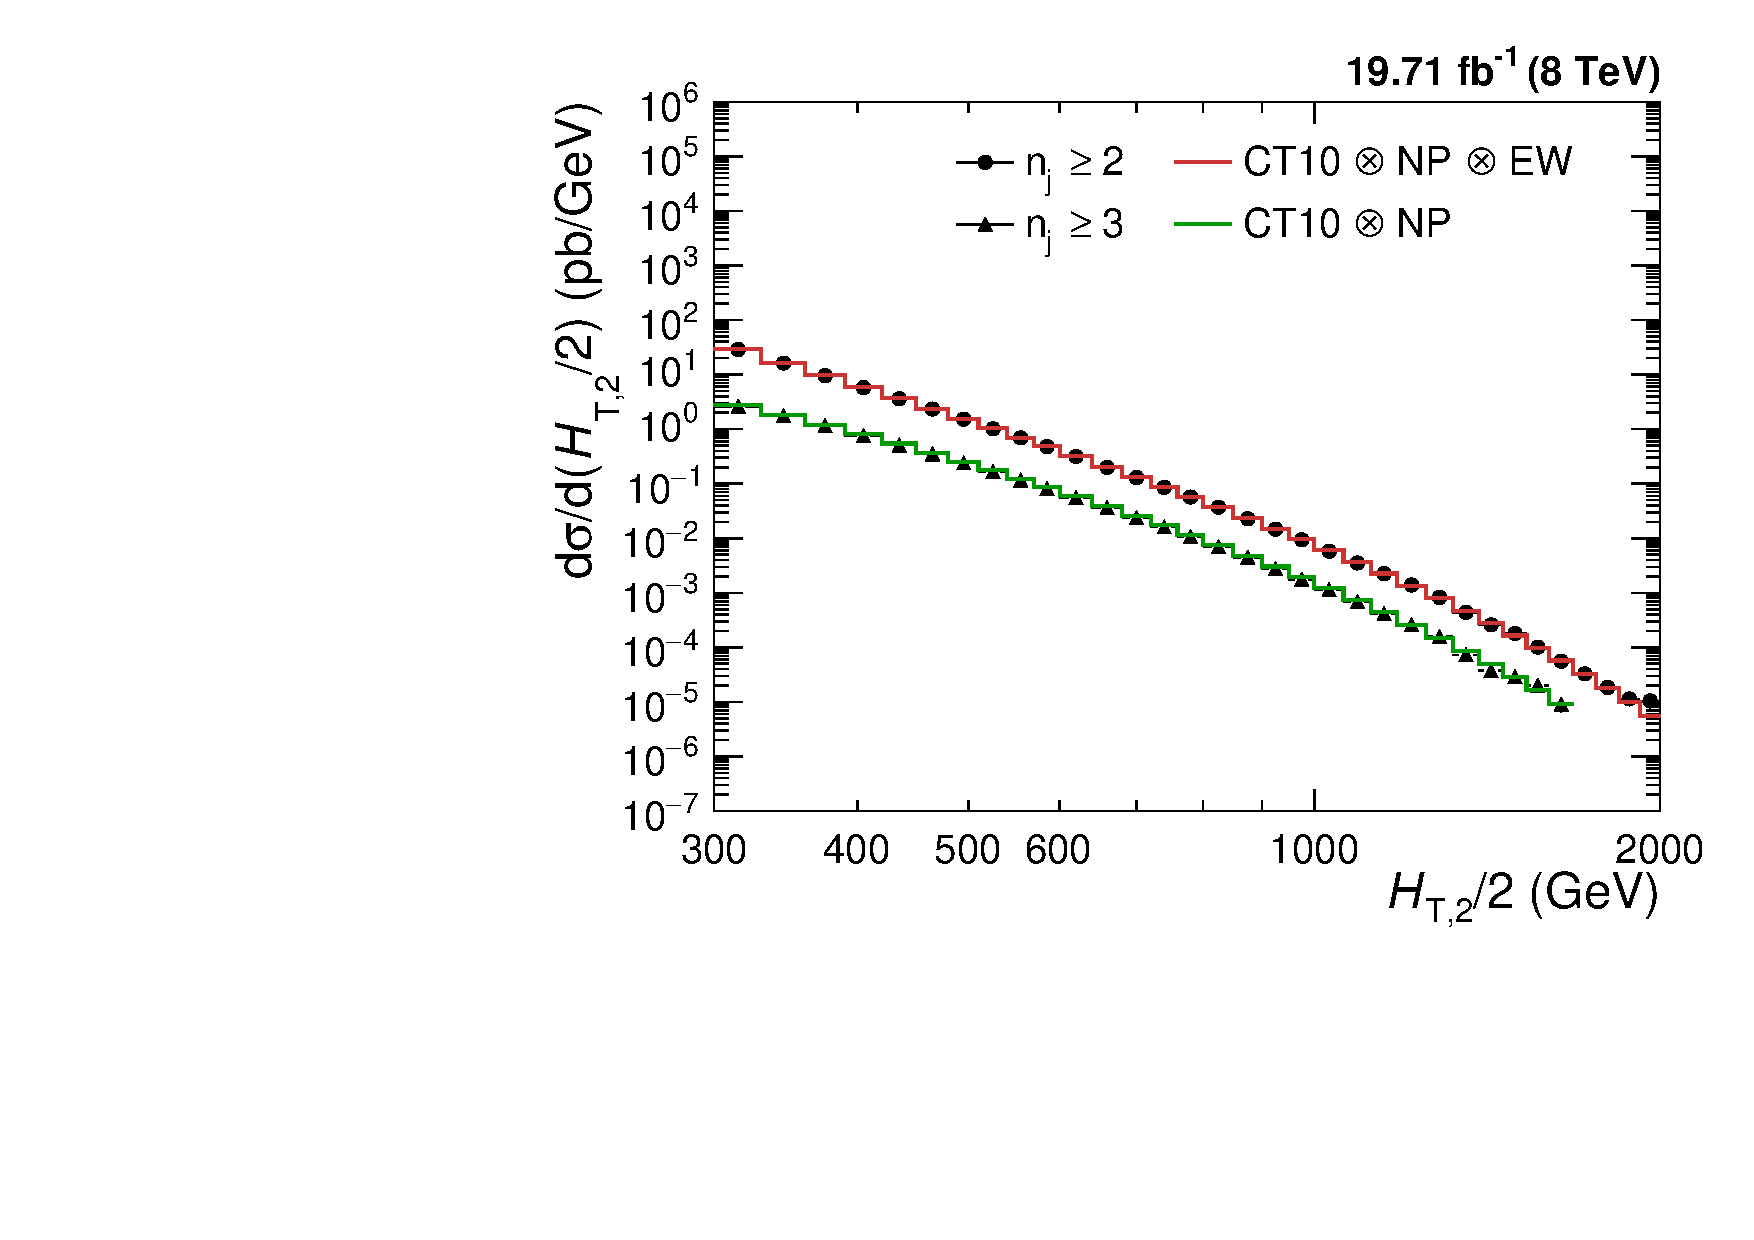
\includegraphics[width=0.51\textwidth]{Plots_HT_2_150/Comparison_data_theory_EW.pdf}%
 ~~\includegraphics[width=0.51\textwidth]{Plots_HT_2_150/Comparison_data_MC_EW.pdf}\\
 \caption{Comparison of the measured differential inclusive 2-jet and 3-jet event cross-sections as a function of \httwo to theoretical predictions. On the left, the data (points) are shown together with \NLOJETPP predictions (line) using the CT10-NLO PDF set, corrected for non-perturbative (NP) and electroweak (EW) effects (2-jet) or only NP effects (3-jet). On the (right), the data (points) are compared to predictions from \MadGraphFn \plusn \PYTHIAS (MG\plusn P6) with tune \Ztwostar (line), corrected for EW effects in the 2-jet case. The error bars give the total experimental uncertainty, given by the quadrature sum of the statistical and systematic uncertainties.}
  \label{fig:data_NL0_MC}
\end{figure}

\begin{figure}[!h]
 \begin{center}
 \includegraphics[width=0.50\textwidth]{Plots_HT_2_150/Sensitivity_ratio_32_CT10_only.pdf}%
 \caption{Cross-section ratio \ratio as a function of \httwo calculated from data (solid circles) in comparison to that from NLO pQCD predictions obtained using the CT10-NLO PDF set corrected with non-perturbative (NP) corrections (line). The error bars correspond to the total experimental uncertainty derived as quadratic sum from all uncertainty sources.}
 \label{fig:ratiosens}
 \end{center}
\end{figure}

Figure~\ref{fig:ratiosens} shows the cross-section ratio \ratio obtained from unfolded data data (solid circles) in comparison to that from NLO pQCD predictions obtained using the CT10-NLO PDF set corrected with NP corrections (line). The error bars here represents the total experimental uncertainty derived as quadratic sum from all uncertainty sources. The deviations of measured \ratio from the theoretical predicted value can be explained by the electroweak effects which are not considered yet because of their unavailability for inclusive 3-jet event cross-sections.

\begin{figure}[!ht]
 \begin{center}
 \hspace*{-5mm}\includegraphics[width=0.51\textwidth]{Plots_HT_2_150/Comparison_data_NLO_Pdfs_2_EW.pdf}%
 ~~\includegraphics[width=0.51\textwidth]{Plots_HT_2_150/Comparison_data_NLO_Pdfs_3.pdf}\\
 \includegraphics[width=0.51\textwidth]{Plots_HT_2_150/Comparison_data_NLO_Pdfs_ratio_32.pdf}\\  
 \caption{Ratio of data over theory using the CT10-NLO PDF set for inclusive 2-jet (top left) and inclusive 3-jet event cross-sections (top right) and their ratio \ratio (bottom). The theory predictions are corrected for non-perturbative effects (NP) and also for electroweak effects (EW) for inclusive 2-jet only. For comparison predictions employing two other PDF sets, MSTW2008 and NNPDF2.3, are also shown. The error bars represents the statistical uncertainty of the data and the shaded rectangles represents the total experimental systematic uncertainty. The shaded band around unity indicate the total uncertainty of the theory.}
 \label{fig:data_NLOPdfs}
 \end{center}  
\end{figure}

For better visibility, the ratios of data over the theory at NLO are also studied in details. In Fig.~\ref{fig:data_NLOPdfs}, the ratios of data over \NLOJETPP predictions using the CT10-NLO PDF set are shown for inclusive 2-jet (top left) and 3-jet event cross-sections (top right) as well as their ratio \ratio (bottom). The data are well described by the predictions within their uncertainty, which is dominated at large \httwo by PDF effects in the upwards and by scale variations in the downwards direction. A trend towards an increasing systematic excess of the 2-jet data with respect to theory, starting at about 1\TeV in \httwo, is remedied by the inclusion of EWK corrections. In the 3-jet case the statistical precision of the data and the reach in \httwo is insufficient to observe any effect. The alternative PDF sets MSTW2008 and NNPDF2.3 exhibit a small underestimation of the cross-sections at high \httwo.

\begin{figure}[!h]
 \begin{center}
 \hspace*{-5mm}\includegraphics[width=0.51\textwidth]{Plots_HT_2_150/Comparison_data_MC_samples_2_Pow_EW.pdf}%
 ~~\includegraphics[width=0.51\textwidth]{Plots_HT_2_150/Comparison_data_MC_samples_3_Pow.pdf}\\
 \includegraphics[width=0.51\textwidth]{Plots_HT_2_150/Comparison_data_MC_samples_ratio_32_Pow.pdf}\\
 \caption{Ratio of data over the prediction from \POWHEGn \plusn \PYTHIAE with tune CUETS1 are presented for inclusive 2-jet (top left) and 3-jet event cross-sections (top right) as well as their ratio \ratio (bottom). For comparison the alternative tune CUETM1 of \POWHEGn \plusn \PYTHIAE, the tree-level multi-leg improved prediction by \MadGraphFn \plusn \PYTHIAS with tune \Ztwostar, and the the LO MC predictions from \PYTHIAS tune \Ztwostar are shown as well. The error bars correspond to the statistical uncertainty of the data and the shaded rectangles to the total experimental systematic uncertainty. EW corrections have been accounted for in this comparison in the 2-jet case only.}
 \label{fig:data_MC}
 \end{center}  
\end{figure}

The \POWHEG~framework providing a NLO dijet calculation matched to the parton showers of \PYTHIAE employed with the CUETS1 and CUETM1 tunes \cite{Khachatryan:2015pea} is also used for a comparison. The ratios of data over theory from \POWHEGn \plusn \PYTHIAE with tune CUETS1 are shown for inclusive 2-jet (top left) and 3-jet event cross-sections (top right) as well as their ratio \ratio (bottom) in Fig.~\ref{fig:data_MC}. For comparison, the LO prediction from \PYTHIAS with tune \Ztwostar, the tree-level multi-leg improved prediction by \MadGraphFn \plusn \PYTHIAS with tune \Ztwostar, and the matched NLO prediction from \POWHEGn \plusn \PYTHIAE with tune CUETM1 are shown as well. EW corrections have been accounted for in this comparison in the 2-jet case only. Significant discrepancies, which are cancelled to a large extent in the ratio \ratio, are visible in the comparison with the LO prediction from \MadGraphFn \plusn \PYTHIAS with tune \Ztwostar, in particular for small \httwo. In contrast, the employed dijet MC \POWHEGn \plusn \PYTHIAE better describe the 2-jet event cross-section, but fail for the 3-jet case.

The jet measurements at hadron colliders can be used to extract the strong coupling constant \alps, which is discussed in the next chapter.

  %Chapter 4	
\chapter{Measurement of the Inclusive Differential Multijet Cross Section}
\label{chap:measurement}
The inclusive differential multijet cross sections are measured as a
function of the average transverse momentum, $\httwo =
\frac{1}{2}(\ptone + \pttwo)$, where \ptone and \pttwo denote the
transverse momenta of the two leading jets. \\

\section{Cross Section Definition}
The inclusive mutijet event yields are transformed into a differential cross section which is defined as :
%
\begin{equation}
  \label{inclusive_formula}
  {\dd{\sigma}{\big(\httwo\big)}} = \frac{1}{\epsilon~\lumi_{\mathrm{int,eff}}}\frac{N_\mathrm{event}}{\Delta\big(\httwo\big)}
\end{equation}
%
where $N_\mathrm{event}$ is the number of 2- or 3-jet events counted in an
\httwo bin, $\epsilon$ is the product of the trigger and jet selection
efficiencies, which are greater than 99\%,
\lumins$_{\mathrm{int,eff}}$ is the effective integrated luminosity,
, and $\Delta\big(\httwo\big)$ are the bin widths. The
measurements are reported in units of (pb/\GeV).

For inclusive 2-jet events
sufficient data are available up to $\httwo = 2\TeV$, while for
inclusive 3-jet events (and the ratio \ratio) the accessible range in
\httwo is limited to $\httwo < 1.68\TeV$. In the following, results
for the inclusive 2-jet and 3-jet event selections will be labelled as
$\mathrm {n_{~j}} \geq 2$ and $\mathrm {n_{~j}} \geq 3$, respectively.

\section{Data Samples}
During 2012, CMS collected data at the center of mass energy $\sqrt{s}$ = 8 TeV in four periods A, B, C, D. The datasets are divided into 
samples according to the run period. For run B-D, the \texttt{JetMon} stream datasets contain prescaled low trigger threshold paths (HLT
PFJet40, 80, 140, 200 and 260) while the \texttt{JetHT} stream datasets contain unprescaled high threshold trigger paths (HLT PFJet320 and 
400). For run A, the \texttt{Jet} stream contains all the above mentioned trigger paths. The datasets used in the current study 
are mentioned in the Table~\ref{tab:dataset} along with the luminosity of each dataset : 

\begin{table}[!htbp]
\centering
\caption{Datasets used along with the corresponding run numbers and luminosity.}
\label{tab:dataset}
\vspace{2mm}
\begin{tabular}{cccc}
\hline\hline
   
Run  & Run Range       &  Dataset                               & Luminosity      \rbthm\\\hline
A    & 190456-193621   & /Jet/Run2012A-22Jan2013-v1/AOD         & 0.88 {\fbinv}   \rbtrr\\
B    & 193834-196531   & /Jet[Mon,HT]/Run2012B-22Jan2013-v1/AOD & 4.49 {\fbinv}   \rbtrr\\
C    & 198022-203742   & /Jet[Mon,HT]/Run2012C-22Jan2013-v1/AOD & 7.06 {\fbinv}   \rbtrr\\
D    & 203777-208686   & /Jet[Mon,HT]/Run2012D-22Jan2013-v1/AOD & 7.37 {\fbinv}   \rbtrr\\
\hline\hline
\end{tabular}
\end{table}

The data sets have the LHC luminosity increasing with period, full data sample of 2012 corresponds to an integrated luminosity of 19.7 {\fbinv}. 

\subsection{Monte Carlo samples}
To have a comparison of data results with the simulated events, the \MadGraphF~\cite{bib:madgraph5} Monte-Carlo event generator has been 
used. The \MadGraphF generates matrix elements for High Energy Physics processes, such as decays and $2 \rightarrow n$ scatterings. The 
underlying event is modeled using the tune \Ztwostar. It has been interfaced to \PYTHIAS~\cite{Sjostrand:2006za} by the LHE event record, 
which generates the rest of the higher-order effects using the Parton Showering (PS) model. Matching algorithms ensure that no double-
counting occurs between the tree-level and the PS-model-generated partons. The MC samples are processed through the complete CMS detector 
simulation to allow studies of the detector response and compare to measured data on detector level.

The cross section measured as a function of the transverse momentum \pt or the scalar sum of the transverse momentum of all jets \HT falls 
steeply with the increasing \pt. So in the reasonable time, it is not possible to generate a large number of high \pt events. Hence, the 
events are generated in the different phase-space region binned in \HT or the leading jet \pt. Later on, the different phase-space regions 
are added together in the data analyses by taking into account the cross section of the different phase-space regions. The official CMS 
\MadGraphF + \PYTHIAS MC samples used in this analysis were generated as slices in the \HT phase-space :
\begin{center}
\begin{itemize}
\item The \MadGraphF + \PYTHIAS MC : /QCD\_HT-xxxtoxxxx\_TuneZ2star\_8TeV-madgraph-pythia6/\\Summer12\_DR53X-PU\_S10\_START53\_V7A-v1/AODSIM
\end{itemize}
\end{center}

 %Chapter 5
%%\chapter{Determination of the Strong Coupling Constant}
\label{chap:Alphas}
The inclusive jet production cross-section at hadron colliders mainly depends on the strong coupling constant \alps for a given centre-of-mass energy. Hence the measurements of the inclusive jet cross-section and jet properties provide a direct probe to measure the strong coupling constant. The measurement of \alps has been already done by various experiments such as CMS~\cite{Chatrchyan:2013txa, Chatrchyan:2013haa, Khachatryan:2014waa, CMS:2014mna, Khachatryan:2016mlc}, ATLAS~\cite{ATLAS:2015yaa}, D0~\cite{Abazov:2009nc, Abazov:2012lua}, H1~\cite{Andreev:2014wwa, Andreev:2016tgi}, and ZEUS~\cite{Abramowicz:2012jz}. In this thesis, the measurements of differential inclusive 2-jet and 3-jet event cross-sections as well as the cross-section ratio \ratio, as a function of \httwo are used to extract the value of the strong coupling constant at  the  scale  of  the  Z boson mass \alpsmz. The differential inclusive jet production cross-section upto at NLO is given by \cite{Affolder:2001hn} :

 \begin{equation}
 \frac{d\sigma}{d(\httwo)} = \alpha_S^2(\mur)\hat{X}^{(0)}(\muf,\httwo)\big[1~\plus \alpha_S(\mur)K1(\mur, \muf,\httwo)\big]
 \label{eqn:SigmaNLO}
 \end{equation}

 where $\frac{d\sigma}{d(\httwo)}$ is the differential inclusive jet production cross-section as a function of \httwo, \mur and \muf are the renormalization and factorization scales set equal to \httwo, $\alpha_S^2(\mur)\hat{X}^{(0)}(\muf,\httwo)$ is the leading order (LO) contribution to the differential inclusive jet production cross-section and $\alpha_S^3(\mur)\hat{X}^{(0)}(\muf,\httwo)K1(\mur, \muf,\httwo)$ is the next-to-leading order (NLO) contribution. Equation~\ref{eqn:SigmaNLO} shows how the inclusive jet production cross-section varies with $\alpha_S(\mur)$. 
 
\section{Sensitivity of Measurements to \texorpdfstring{\alpsmz}{alpha-S(M(Z))}}
\label{sec:sensitivity}
 
For a fixed choice of \mur and \muf, different input values of \alpsmz to a PDF set will lead to different theory predictions of the differential cross-section distribution. This will give an estimate of the sensitivity of the theory predictions to the varying input value of \alpsmz. A comparison of the measured spectrum with the theory predictions obtained using all \alpsmz inputs will give a hint of the input value of \alpsmz for which the theory distribution has the closest matching with data. In this section, the sensitivity of the inclusive differential jet event cross-sections and cross-section ratio, \ratio to varying input values of \alpsmz for different PDF sets is demonstrated by plotting the ratios of data over theory predictions with central value of \alpsmz.

Figures~\ref{fig:sensitivity_2},~\ref{fig:sensitivity_3} and~\ref{fig:sensitivity_double_ratio} present the ratio of data to the theory predictions, corrected for NP effects, for all variations in \alpsmz available for the PDF sets CT10, CT14, MSTW2008, MMHT2014 and NNPDF2.3 at NLO evolution order as specified in Table~\ref{tab:nlopdfsets}, for inclusive 2-jet event cross-sections, inclusive 3-jet events cross-sections and ratio \ratio respectively. The \alpsmz value is varied in the range 0.112-0.127, 0.111-123, 0.110-0.130, 0.108-0.128 and 0.114-0.124 in steps of 0.001 for the CT10, CT14, MSTW2008, MMHT2014 and NNPDF2.3PDF sets, respectively. The error bars correspond to the total experimental uncertainty derived as quadratic sum from all uncertainty sources. The theory predictions are also corrected for EW effects for inclusive 2-jet events cross-section. A small slope increasing with \httwo is visible for most PDFs in both cross-sections. This effect is largely cancelled in the cross-section ratio. \ratio exhibits a flat behaviour with respect to the predictions for all five PDF sets in the whole range of \httwo up to 1680 GeV. Therefore, these data can be used to determine the strong coupling constant, although only up to 1 TeV for the cross-sections as long as electroweak corrections are not taken into account.

Moreover, the different sensitivity to \alpsmz caused by the leading power in \alps in the expansion of the 2-jet inclusive ($\propto\alps^2$) and the 3-jet inclusive cross-section ($\propto\alps^3$), and their ratio ($\propto\alps^1$) is clearly visible from the spread between the calculations for the smallest and largest value of \alpsmz within the same PDF set when passing through Figures~\ref{fig:sensitivity_2}--\ref{fig:sensitivity_double_ratio}.  This also demonstrates the potential of ratios $R_{mn}$ with $m$-$n$ \gr 1.

\begin{figure}[!htbp]
 \begin{center}
 \hspace*{-5mm}\includegraphics[width=0.51\textwidth]{Plots_HT_2_150/Sensitivity_2_ratio_NLO_CT10_EW.pdf}%
 ~~\includegraphics[width=0.51\textwidth]{Plots_HT_2_150/Sensitivity_2_ratio_NLO_CT14_EW.pdf}\\
 \vspace*{3mm}
 \hspace*{-5mm}\includegraphics[width=0.51\textwidth]{Plots_HT_2_150/Sensitivity_2_ratio_NLO_MSTW2008_EW.pdf}%
 ~~\includegraphics[width=0.51\textwidth]{Plots_HT_2_150/Sensitivity_2_ratio_NLO_MMHT2014_EW.pdf}\\
 \vspace*{3mm}
 \includegraphics[width=0.51\textwidth]{Plots_HT_2_150/Sensitivity_2_ratio_NLO_NNPDF23_EW.pdf}
 \caption{Ratio of the inclusive 2-jet differential cross-section to theory predictions using the CT10 (top left), the CT14 (top right), the MSTW2008 (middle left), the MMHT2014 (middle right) and NNPDF2.3 (bottom) NLO PDF sets for a series of values of \alpsmz. The \alpsmz value is varied in the range 0.112-0.127, 0.111-123, 0.110-0.130, 0.108-0.128 and 0.114-0.124 in steps of 0.001 for the CT10, CT14, MSTW2008, MMHT2014 and NNPDF2.3 NLO PDF sets, respectively. The error bars correspond to the total experimental uncertainty. The theory predictions are corrected for non-perturbative (NP) and electroweak (EW) effects.}
 \label{fig:sensitivity_2}
 \end{center}
\end{figure}

\begin{figure}[!htbp]
 \begin{center}
 \hspace*{-5mm}\includegraphics[width=0.51\textwidth]{Plots_HT_2_150/Sensitivity_3_ratio_NLO_CT10.pdf}%
 ~~\includegraphics[width=0.51\textwidth]{Plots_HT_2_150/Sensitivity_3_ratio_NLO_CT14.pdf}\\
 \vspace*{3mm}
 \hspace*{-5mm}\includegraphics[width=0.51\textwidth]{Plots_HT_2_150/Sensitivity_3_ratio_NLO_MSTW2008.pdf}%
 ~~\includegraphics[width=0.51\textwidth]{Plots_HT_2_150/Sensitivity_3_ratio_NLO_MMHT2014.pdf}\\
 \vspace*{3mm}
 \includegraphics[width=0.51\textwidth]{Plots_HT_2_150/Sensitivity_3_ratio_NLO_NNPDF23.pdf}
 \caption{Ratio of the inclusive 3-jet differential cross-section to theory predictions using the CT10 (top left), the CT14 (top right), the MSTW2008 (middle left), the MMHT2014 (middle right) and NNPDF2.3 (bottom) NLO PDF sets for a series of values of \alpsmz. The \alpsmz value is varied in the range 0.112-0.127, 0.111-123, 0.110-0.130, 0.108-0.128 and 0.114-0.124 in steps of 0.001 for the CT10, CT14, MSTW2008, MMHT2014 and NNPDF2.3 NLO PDF sets, respectively. The error bars correspond to the total experimental uncertainty. The theory predictions are corrected for non-perturbative (NP) effects.}
 \label{fig:sensitivity_3}
 \end{center}
\end{figure}

\begin{figure}[!htbp]
 \begin{center}
 \hspace*{-5mm}\includegraphics[width=0.51\textwidth]{Plots_HT_2_150/Sensitivity_double_ratio_32_CT10.pdf}%
 \includegraphics[width=0.51\textwidth]{Plots_HT_2_150/Sensitivity_double_ratio_32_CT14.pdf}\\
 \vspace*{3mm}
 \hspace*{-5mm}\includegraphics[width=0.51\textwidth]{Plots_HT_2_150/Sensitivity_double_ratio_32_MSTW2008.pdf}%
 \includegraphics[width=0.51\textwidth]{Plots_HT_2_150/Sensitivity_double_ratio_32_MMHT2014.pdf}\\
 \vspace*{3mm}
 \includegraphics[width=0.51\textwidth]{Plots_HT_2_150/Sensitivity_double_ratio_32_NNPDF23.pdf}
 \caption{Ratio of the cross-section ratio, \ratio to theory predictions using the CT10 (top left), the CT14 (top right), the MSTW2008 (middle left), the MMHT2014 (middle right) and NNPDF2.3 (bottom) NLO PDF sets for a series of values of \alpsmz. The \alpsmz value is varied in the range 0.112-0.127, 0.111-123, 0.110-0.130, 0.108-0.128 and 0.114-0.124 in steps of 0.001 for the CT10, CT14, MSTW2008, MMHT2014 and NNPDF2.3 NLO PDF sets, respectively. The error bars correspond to the total experimental uncertainty. The theory predictions are corrected for non-perturbative (NP) effects.}
 \label{fig:sensitivity_double_ratio}
 \end{center}
\end{figure}

\section{Determination of \texorpdfstring{\alpsmz}{alpha-S(M(Z))}}

As discussed in the previous section, the measured inclusive 2-jet and 3-jet event cross-sections and their ratio \ratio can be used for a determination of the strong coupling constant \alpsmz. To extract the value of \alpsmz, a general fit procedure \cite{Chatrchyan:2013txa,Khachatryan:2014waa} has been followed and is described in the following section. 

\subsection{Fitting Procedure}
\label{sec:Fits_procedure}
The value of \alpsmz is determined by minimizing the chi-square (\chisq) between the experimental measurement and the theoretical predictions. The \chisq is defined as:

\begin{equation}
  \label{chisq}
  \chisq = M^{T}C^{-1}M
\end{equation}
where $M$ is the vector of the differences between the data ($D^{i}$) and the theoretical values ($T^{i}$) in each bin $i$,

\begin{equation}
 \label{eqn:M_matrix}
 M^{i}=D^{i}-T^{i}
\end{equation}
and $C$ is the covariance matrix including all experimental uncertainties as described in Sec.~\ref{sec:exp_unc} and some theoretical uncertainties discussed in Sec.~\ref{sec:theory_unc}. The covariance matrix $C=C_\mathrm{exp}~\plus C_\mathrm{theo}$ is defined as the sum of covariances of experimental and theoretical sources of uncertainty as follows : 

\begin{eqnarray}
 \label{eqn:c_exp}
 C_\mathrm{exp} &=& \mathrm{Cov}^\mathrm{ExpStat}~\plus \sum\mathrm{Cov}^\mathrm{JEC}~\plus \mathrm{Cov}^\mathrm{Unfolding}~\plus \mathrm{Cov}^\mathrm{Lumi}~\plus \mathrm{Cov}^\mathrm{Residual}\\
 C_\mathrm{theo} &=& \mathrm{Cov}^\mathrm{TheoStat}~\plus \mathrm{Cov}^\mathrm{NP}~\plus \mathrm{Cov}^\mathrm{PDF}
 \label{eqn:c_theo}
\end{eqnarray}
where the labelled covariance matrices account for the following effects:

\begin{itemize}
\item{$\mathrm{Cov}^\mathrm{ExpStat}$: statistical uncertainty of the data including correlations introduced by the unfolding}
\item{$\mathrm{Cov}^\mathrm{JEC}$: the jet energy corrections (JEC) systematic uncertainty}
\item{$\mathrm{Cov}^\mathrm{Unfolding}$: the unfolding systematic uncertainty including the resolution (JER) and model dependence}
\item{$\mathrm{Cov}^\mathrm{Lumi}$: the luminosity uncertainty}
\item{$\mathrm{Cov}^\mathrm{Residual}$: a residual uncorrelated systematic uncertainty summarizing individual causes such as small trigger and identification inefficiencies, time dependence of the jet \pt resolution, and uncertainty on the trigger prescale factors}
\item{$\mathrm{Cov}^\mathrm{TheoStat}$: statistical uncertainty caused by numerical integrations in the cross-section computations}
\item{$\mathrm{Cov}^\mathrm{NP}$: the systematic uncertainty of the non-perturbative (NP) corrections}
\item{$\mathrm{Cov}^\mathrm{PDF}$: the PDF uncertainties}
\end{itemize}

While taking the differences between theory and data, the treatment of experimental and theoretical systematic uncertainties is crucial. The Unfolding, JEC, Lumi and PDF and NP systematic uncertainties are treated as 100$\%$ correlated among \httwo bins. If $\delta_i$ is the total uncertainty on the differential cross-section, for the $i$-th \httwo bin, for any of these fully correlated sources, then the$i,j$-th element of the corresponding covariance matrix is given by COV$_{ij} = \delta_i \times \delta_j$. The JEC, unfolding, and luminosity uncertainties are treated as multiplicative to avoid the statistical bias that arises when estimating uncertainties from data. In fits of the ratio \ratio, the luminosity and residual uncorrelated uncertainties cancel completely. Partial cancellations between the other sources of uncertainty are taken into account in the fit. 

The evaluation of PDF uncertainty depends on the individual PDF set as already discussed in Sec.~\ref{sec:pdf_unc}. The PDF covariance matrix construction varies among different PDF sets. The CT10, CT14, MMHT2014 and MSTW2008 NLO PDF sets employ the eigenvector method to evaluate the PDF uncertainties as explained in Sec.~\ref{sec:pdf_unc}. The number of eigenvectors ($N_\mathrm{ev}$) with two PDF members per eigenvector for CT10, CT14, MMHT2014 and MSTW2008 NLO PDF sets are 26, 28, 25 and 20, respectively. The NNPDF2.3 PDF set comes with hundred different replicas ($N_{rep}$) instead of different eigenvectors, as for CT10 or CT14 PDF sets. The mean uncertainty is calculated as average uncertainty from 100 different replicas. Following the prescription given in~\cite{Ball:2010de}, the PDF uncertainty is calculated as :

\begin{equation}
(\Delta X)^2 = \frac{1}{N_{rep}-1} \sum_{k=1}^{N_{rep}} [X_k - \langle X_k \rangle]^2
\end{equation}

where $\Delta X$ is the uncertainty on predicted differential cross-section, $X_k$ is the differential cross-section for $k$-th replica and $\langle X_k \rangle$ is the average differential cross-section from all the replicas. 

Scale uncertainties of the pQCD predictions are taken into account by employing the offset method, \ie by performing separate fits with varying scale factors as described in the Sec.~\ref{sec:scale_unc}. The largest upwards and downwards deviations from the default factors are defined as the uncertainty. At NLO such scale variations predominantly lead to smaller cross-sections and also a smaller ratio \ratio as visible in Fig.~\ref{fig:theory_unc}. As a consequence the scale uncertainty in fits is equally asymmetric, where smaller cross-sections or ratios are compensated by an increase in the fitted value for \alpsmz.

\subsection{Fit Results}
To determine the value of the strong coupling constant at the scale of the Z boson mass \alpsmz, fits to the differential inclusive 2-jet and 3-jet events cross-sections are performed using five different NLO PDF sets : CT10, CT14, MSTW2008, MMHT2014 and NNPDF2.3. The range in \httwo is restricted to be between 300 GeV and 1 TeV to avoid the region close to the minimal \pt threshold of 150 GeV for each jet at low \pt and the onset of electroweak effects at high \httwo, which are available for the dijet case only. The \alpsmz results obtained from a simultaneous fit to all 19 \httwo bins in the above mentioned range are reported in Table~\ref{tab:xsep300-1000}. For comparison, a simultaneous fit to both cross-sections ignoring any correlations, and a fit to the cross-section ratio \ratio, fully accounting for correlations is also performed and the results are tabulated in Table~\ref{tab:xcomb300-1000}. The electroweak effects are assumed to cancel in the ratio as do the luminosity and the uncorrelated uncertainty.

All cross-section fits give compatible values for \alpsmz in the range of 0.115-0.118 whereas for the ratio \ratio somewhat smaller values are obtained. But for individual cross-sections, \chisqndof values are small as compared to the cross-section ratio \ratio. A possible explanation is an overestimation of the residual uncorrelated uncertainty of 1\% that is cancelled for \ratio. If the fits are repeated with an assumed uncertainty of 0.25\% instead, the \chisqndof values lie around unity while the \alpsmz values are still compatible with the previous results but with slightly reduced uncertainties. 
%
% 300 - 1000 GeV
%
\begin{table}[htbp]
  \caption{Determination of \alpsmz from the inclusive 2-jet and 3-jet event cross-sections using five PDF sets at NLO\@. Only total uncertainties without scale variations are quoted. The results are obtained from a simultaneous fit to all 19 \httwo bins in the restricted range of $0.3 < \httwo < 1.0$ TeV.}
  \label{tab:xsep300-1000}
  \centering
  \vspace{2mm} 
  \begin{tabular}{l|ccc|ccc}
    \hline\hline
    \multirow{2}{*}{PDF set} & \multicolumn{3}{c|}{Inclusive 2-jets} & \multicolumn{3}{c}{Inclusive 3-jets} \\
    & \alpsmz & $\pm\Delta\alpsmz$ & \chisqndof &\alpsmz & $\pm\Delta\alpsmz$ & \chisqndof \\\hline
    CT10           & 0.1174 & 0.0032 & 3.0/18 & 0.1169 & 0.0027 & 5.4/18 \rbtrr\\
    CT14           & 0.1160 & 0.0035 & 3.5/18 & 0.1159 & 0.0031 & 6.1/18 \rbtrr\\
    MSTW2008       & 0.1159 & 0.0025 & 5.3/18 & 0.1161 & 0.0021 & 6.7/18 \rbtrr\\
    MMHT2014       & 0.1165 & 0.0034 & 5.9/18 & 0.1166 & 0.0025 & 7.1/18 \rbtrr\\
    NNPDF2.3       & 0.1183 & 0.0025 & 9.7/18 & 0.1179 & 0.0021 & 9.1/18 \rbtrr\\
    \hline\hline
  \end{tabular}
\end{table}

\begin{table}[htbp]
  \caption{Determination of \alpsmz from the inclusive 2-jet and 3-jet event cross-sections simultaneously and from their ratio \ratio using five PDF sets at NLO\@. Only total uncertainties without scale variations are quoted. The results are obtained from a simultaneous fit to all 38 (left) and 19 (right) \httwo bins in the restricted range of $0.3 < \httwo < 1.0$ TeV. For comparison, correlations between the two cross-sections are neglected in the simultaneous fit on the left, but fully taken into account in the ratio fit on the right.}
  \label{tab:xcomb300-1000}
  \centering
  \vspace{2mm}  
  \begin{tabular}{l|ccc|ccc}
    \hline\hline
    \multirow{2}{*}{PDF set} & \multicolumn{3}{c|}{Inclusive 2- and 3-jets} & \multicolumn{3}{c}{\ratio} \\
    & \alpsmz & $\pm\Delta\alpsmz$ & \chisqndof &\alpsmz & $\pm\Delta\alpsmz$ & \chisqndof \\\hline
    CT10           & 0.1170 & 0.0026 & 8.2/37 & 0.1141 & 0.0028 & 19./18 \rbtrr\\
    CT14           & 0.1161 & 0.0029 & 9.1/37 & 0.1139 & 0.0032 & 15./18 \rbtrr\\
    MSTW2008       & 0.1161 & 0.0021 & 11./37 & 0.1150 & 0.0023 & 21./18 \rbtrr\\
    MMHT2014       & 0.1168 & 0.0025 & 11./37 & 0.1142 & 0.0022 & 19./18 \rbtrr\\
    NNPDF2.3       & 0.1188 & 0.0019 & 15./37 & 0.1184 & 0.0021 & 12./18 \rbtrr\\
    \hline\hline
  \end{tabular}
\end{table}

To investigate how the electroweak (EW) corrections affect the fit results for \alpsmz, the range in \httwo is extended to $0.3 < \httwo < 1.68$ TeV. \alpsmz values are obtained from fits to the inclusive 2-jet event cross-section in this range with or without EW correction factors and the results are presented in Table~\ref{tab:xsep300-1680}. The largest impact is a reduction in \chisqndof, which indicates a better agreement when EW effects are included. In addition, a tendency to slightly smaller \alpsmz values is observed without the EW corrections. For the ratio \ratio, it is expected that these effects are much reduced. 
%
% 300 - 1680 GeV, 2j only, w/o ew
%
\begin{table}[htbp]
  \caption{Determination of \alpsmz from the inclusive 2-jet event cross-section using five PDF sets at NLO without (left) and with (right) electroweak (EW) corrections. Only total uncertainties without scale variations are quoted. The results are obtained from a simultaneous fit to all 29 \httwo bins in the range of $0.3 < \httwo < 1.68$ TeV.}
 \label{tab:xsep300-1680}
 \centering
 \vspace{2mm}
 \begin{tabular}{l|ccc|ccc}
 \hline\hline
 \multirow{2}{*}{PDF set} & \multicolumn{3}{c|}{without EW} &
 \multicolumn{3}{c}{with EW} \\
 & \alpsmz & $\pm\Delta\alpsmz$ & \chisqndof &\alpsmz & $\pm\Delta\alpsmz$ & \chisqndof \\\hline
 CT10           & 0.1163 & 0.0034 & 15./28 & 0.1165 & 0.0032 & 14./28 \rbtrr\\
 CT14           & 0.1137 & 0.0033 & 24./28 & 0.1144 & 0.0033 & 17./28 \rbtrr\\
 MSTW2008       & 0.1093 & 0.0028 & 27./28 & 0.1133 & 0.0023 & 19./28 \rbtrr\\
 MMHT2014       & 0.1127 & 0.0032 & 32./28 & 0.1141 & 0.0032 & 21./28 \rbtrr\\
 NNPDF2.3       & 0.1162 & 0.0024 & 31./28 & 0.1168 & 0.0024 & 23./28 \rbtrr\\
 \hline\hline
 \end{tabular}
\end{table}

From Fig.~\ref{fig:sensitivity_double_ratio} follows that only the PDF sets MSTW2008 and MMHT2014 provide a large enough range in \alpsmz values to ensure fits without extrapolation. The other three PDF sets are at the limit such that reliable fits cannot be performed for all scale settings and/or bins in scale $Q=\httwo$. Since many systematic uncertainties cancel completely or partially in the cross-section ratio \ratio as compared to the individual cross-sections, \ratio is used mainly to determine the value of \alpsmz. Table~\ref{tab:xcomb300-1680} give the complete results for MSTW2008 and MMHT2014 for the full range in \httwo of 300 GeV up to 1.68 TeV along with the corresponding components of PDF, scale, NP and total experimental except scale uncertainties are shown. In contrast to fits at NLO using cross-sections where the scale uncertainty recipe usually leads to a very asymmetric behaviour with larger downward uncertainties in the case, this is inverted for the fits to the cross-section ratio \ratio. The scale uncertainty is the most dominant source of total uncertainty on \alpsmz. These values are determined with the central renormalization and factorization scales i.e. \mur = \muf = \httwo. The values are also determined for the six scale factor combinations for the two PDF sets MSTW2008 and MMHT2014 ans results are shown in Table~\ref{tab:as_values_scalevar}. The uncertainty decomposition for \alpsmz determined from cross-section ratio \ratio is performed in four sub-ranges of \httwo and the results are shown in Table~\ref{tab:as_values_qbins}. The statistical uncertainty of the NLO computation is negligible in comparison to any of the other sources of uncertainty. Electroweak corrections, significant only at high \httwo, are assumed to cancel between the numerator and denominator. 
%
% 300 - 1680 GeV, R_32 only, only MSTW/MMHT, pol2, asredrange
%
% Base fit
%
\begin{table}[p]
 \caption{Determination of \alpsmz from the ratio \ratio using the two most compatible PDF sets MSTW2008 and MMHT2014 at NLO along with the corresponding components of PDF, scale, NP and total (except scale) experimental uncertainties. The results are obtained from a simultaneous fit to all 29 \httwo bins in the full range of $0.3 < \httwo < 1.68$ TeV.} 
 \label{tab:xcomb300-1680}
 \centering
 \vspace{2mm}
 %\begin{tabular}{lc|ccccc|c}
 \begin{tabular}{lccccccc}
 \hline\hline
 %&  & \multicolumn{5}{c|}{$\Delta\alpsmz$} & \\
 PDF set & \alpsmz & exp & PDF & NP & all exc.\ scale & scale & \chisqndof \rbthm\\\hline
 %MSTW2008       & 0.1150 & $\pm10$ & $\pm13$ & $\pm15$ & $\pm23$ & $^{+50}_{-0}$ & 26./28 \rbtrr\\
 %MMHT2014       & 0.1142 & $\pm10$ & $\pm13$ & $\pm14$ & $\pm22$ & $^{+49}_{-6}$ & 24./28 \rbtrr\\
 MSTW2008       & 0.1150 & $\pm$0.0010 & $\pm$0.0013 & $\pm$0.0015 & $\pm$0.0023 & $^{+0.0050}_{-0.0000}$ & 26./28 \rbtrr\\
 MMHT2014       & 0.1142 & $\pm$0.0010 & $\pm$0.0013 & $\pm$0.0014 & $\pm$0.0022 & $^{+0.0049}_{-0.0006}$ & 24./28 \rbtrr\\
 \hline\hline
 \end{tabular}
\end{table}
%
% Scale variations
%
\begin{table}[htbp]
 \caption{Determination of \alpsmz from the ratio \ratio in the \httwo range from 0.3 up to 1.68 TeV at the central scale and for the six scale factor combinations for the two PDF sets MSTW2008 and MMHT2014.}
 \label{tab:as_values_scalevar}
 \centering
 \vspace{2mm}
 \begin{tabular}{cccccc}
 \hline\hline
 \multirow{2}{*}{$\mur/\httwo$} & \multirow{2}{*}{$\muf/\httwo$} &
 \multicolumn{2}{c}{MSTW2008} & \multicolumn{2}{c}{MMHT2014}\rbtrr\\
 & & \alpsmz & \chisqndof & \alpsmz & \chisqndof\rbthm\\\hline
 $1$    & $1$    & $0.1150$ & $26./28$ & $0.1142$ & $24./28$\rbtrr\\
 $1/2$  & $1/2$  & $0.1165$ & $77./28$ & $0.1160$ & $73./28$\rbtrr\\
 $2$    & $2$    & $0.1200$ & $18./28$ & $0.1191$ & $18./28$\rbtrr\\
 $1/2$  & $1$    & $0.1150$ & $53./28$ & $0.1136$ & $48./28$\rbtrr\\
 $1$    & $1/2$  & $0.1150$ & $30./28$ & $0.1142$ & $28./28$\rbtrr\\
 $1$    & $2$    & $0.1155$ & $23./28$ & $0.1147$ & $22./28$\rbtrr\\
 $2$    & $1$    & $0.1180$ & $19./28$ & $0.1175$ & $19./28$\rbtrr\\
 \hline\hline
 \end{tabular}
\end{table}
%
% Q bins
%
\begin{table}[htbp]
 \caption{Uncertainty decomposition for \alpsmz from the determination of \alps from the jet event rate \ratio in bins of \httwo. The statistical uncertainty of the NLO computation is negligible in comparison to any of the other sources of uncertainty. Electroweak corrections, significant only at high \httwo, are assumed to cancel between the numerator and denominator.} 
 \label{tab:as_values_qbins}
 \centering
  \vspace{2mm}
 %\begin{tabular}{c|ccccc|ccccc}
 \hspace*{-8mm}
 \begin{tabular}{>{\centering\arraybackslash}m{0.71in}|>{\centering\arraybackslash}m{0.4in}>{\centering\arraybackslash}m{0.47in} >{\centering\arraybackslash}m{0.47in} >{\centering\arraybackslash}m{0.45in} >{\centering\arraybackslash}m{0.45in}| >{\centering\arraybackslash}m{0.4in}>{\centering\arraybackslash}m{0.47in} >{\centering\arraybackslash}m{0.47in}>{\centering\arraybackslash}m{0.45in}>{\centering\arraybackslash}m{0.45in}}
 \hline\hline
 \httwo & % $\langle{}Q\rangle$ &
    \multicolumn{5}{c|}{MSTW2008} &
    \multicolumn{5}{c}{MMHT2014} \\
    (GeV) & % (\GeV) &
    \alpsmz & exp & PDF & NP & scale &
    \alpsmz & exp & PDF & NP & scale \rbthm\\\hline
    300-420 \rbtrr  & %474 &
    0.1157 & $\pm{0.0015}$ & $\pm{0.0014}$    & $\pm{0.0019}$     & $^{+0.0053}_{-0.0000}$ &
    0.1158 & $\pm{0.0014}$ & $\pm{0.0010}$    & $\pm{0.0019}$     & $^{+0.0052}_{-0.0000}$\\
    420-600 \rbtrr  & %664 &
    0.1153 & $\pm{0.0011}$ & $\pm{0.0014}$    & $\pm{0.0018}$     & $^{+0.0057}_{-0.0000}$ &
    0.1154 & $\pm{0.0011}$ & $\pm{0.0012}$    & $\pm{0.0017}$     & $^{+0.0056}_{-0.0000}$\\
    600-1000\rbtrr  & %896 &
    0.1134 & $\pm{0.0013}$ & $\pm{0.0016}$    & $\pm{0.0019}$     & $^{+0.0052}_{-0.0000}$ &
    0.1140 & $\pm{0.0012}$ & $\pm{0.0012}$    & $\pm{0.0018}$     & $^{+0.0045}_{-0.0000}$\\
    1000-1680\rbtrr & %896 &
    0.1147 & $\pm{0.0029}$ & $\pm{0.0017}$    & $\pm{0.0018}$     & $^{+0.0063}_{-0.0011}$ &
    0.1154 & $\pm{0.0025}$ & $\pm{0.0014}$    & $\pm{0.0015}$     & $^{+0.0056}_{-0.0011}$\\\hline
    300-1680\rbtrr  & %896 &
    0.1150 & $\pm{0.0010}$ & $\pm{0.0013}$    & $\pm{0.0015}$     & $^{+0.0050}_{-0.0000}$ &
    0.1142 & $\pm{0.0010}$ & $\pm{0.0013}$    & $\pm{0.0014}$     & $^{+0.0049}_{-0.0006}$\\
    \hline\hline
 \end{tabular}
\end{table}

Using the MSTW2008 PDF set, which dates from before the LHC start, the strong coupling constant finally is determined to

\begin{equation}
\begin{gathered}
  \alpsmz = 0.1150\,\pm0.0010\,\textrm{(exp)}\,\pm0.0013\,\textrm{(PDF)}\,\pm0.0015\,\textrm{(NP)}\,^{+0.0050}_{-0.0000}\,\textrm{(scale)}\\
  \hspace*{-20mm} = 0.1150\,\pm0.0023\,\textrm{(all except scale)}\,^{+0.0050}_{-0.0000}\,\textrm{(scale)}\,
\end{gathered}
\end{equation}

The MMHT2014 PDF set, although using LHC jet data to determine the PDF parameters, leads to a very similar result of
\begin{equation}
\begin{gathered}
  \alpsmz = 0.1142\,\pm0.0010\,\textrm{(exp)}\,\pm0.0013\,\textrm{(PDF)}\,\pm0.0014\,\textrm{(NP)}\,^{+0.0049}_{-0.0006}\,\textrm{(scale)}\\
  \hspace*{-20mm} = 0.1142\,\pm0.0022\,\textrm{(all except scale)}\,^{+0.0049}_{-0.0006}\,\textrm{(scale)}\,
\end{gathered}
\end{equation}

\section{Running of the Strong Coupling Constant}
The value of the strong coupling constant \alps depends on the energy scale Q and it decreases with the increase of scale Q. To study this dependence, the determination of \alps is carried out at different energies. The procedure to extract \alpsq is same as the one followed for the \alpsmz. To have different energy scales, the fitted \httwo range 300 - 1680 GeV is divided into four different sub-ranges as shown by the first column in Table~\ref{tab:asq_values}. Each of the \httwo range is associated with a scale Q, which is the differential cross-section weighted average \httwo scale from the inclusive 2-jet calculations and integrated over all the measured \httwo bins contributing to that given \httwo range. Let $N^{j}_{bin}$ be the total number of measured \httwo bins contributing to the $j$-th \httwo range, then the corresponding scale Q$_{j}$, shown in second column of Table~\ref{tab:asq_values}, is calculated as :
%\frac[10pt]
\begin{equation}
Q_{j} = \frac[10pt]{\sum\limits_{i=1}^{N^{j}_{bin}} H^{i}_{\rm T,2} \bigg[{\dd{\sigma}{(\httwo)}}\bigg]^{i}}{\sum\limits_{i=1}^{N^{j}_{bin}} \bigg[{\dd{\sigma}{(\httwo)}}\bigg]^{i}}
\end{equation}

The value of \alpsmz is extracted in each \httwo range. These extracted \alpsmz values are evolved to the corresponding values \alpsq and are quoted in Table~\ref{tab:asq_values} along with the extracted \alpsmz values and the total uncertainty. The evolution is performed for five flavours at 2-loop order with the \RunDec program~\cite{Chetyrkin:2000yt, Schmidt:2012az}. The obtained \alpsq points (black solid circles) are shown as a function of scale Q in Fig.~\ref{fig:running_alphas}. The black solid line and the yellow uncertainty band are evolved using \alpsmz = $0.1150\,\pm0.0023\,\textrm{(all except scale)}\,^{+0.0050}_{-0.0000}\,\textrm{(scale)}$ obtained using MSTW2008 NLO PDF set. The world average~\cite{Patrignani:2016xqp} (dashed line) and results from other measurements of the CMS~\cite{Chatrchyan:2013txa, Chatrchyan:2013haa, Khachatryan:2014waa, CMS:2014mna, Khachatryan:2016mlc}, ATLAS~\cite{ATLAS:2015yaa}, D0~\cite{Abazov:2009nc, Abazov:2012lua}, H1~\cite{Andreev:2014wwa, Andreev:2016tgi}, and ZEUS~\cite{Abramowicz:2012jz} experiments are also imposed. The current measurement is in very good agreement within the uncertainty with other results obtained by previous experiments as well as with the world average value of $\alpsmz = 0.1181 \,\pm\, 0.0011$ derived in Ref.~\cite{Patrignani:2016xqp}.
%
% alpha_s(Q) bins
%
\begin{table}[htbp]
 \caption{Evolution of the strong coupling constant between the scale of the Z boson mass and the cross-section averaged \httwo scale $\langle{}Q\rangle$ for the separate determinations in each respective fit range. The evolution is performed for five flavours at 2-loop order with the \RunDec program~\cite{Chetyrkin:2000yt, Schmidt:2012az}.}
 \label{tab:asq_values}
 \centering
 \vspace{2mm}
 \begin{tabular}{cccccc}
    \hline\hline
    \httwo & $\langle{}Q\rangle$ & \alpsmz & \alpsq & No.\ of data & \chisqndof\\
    (GeV) & (GeV) & & & points & \rbthm\\\hline
    % v4
    300-420 \rbtrr  &  340 &
    $0.1157\,^{+0.0060}_{-0.0030}$ & $0.0969\,^{+0.0041}_{-0.0021}$ &  4 & 2.8/3 \\
    420-600 \rbtrr  &  476 &
    $0.1153\,^{+0.0062}_{-0.0025}$ & $0.0928\,^{+0.0039}_{-0.0016}$ &  6 & 6.1/5 \\
    600-1000\rbtrr  &  685 &
    $0.1134\,^{+0.0059}_{-0.0028}$ & $0.0879\,^{+0.0035}_{-0.0017}$ &  9 & 7.1/8 \\
    1000-1680\rbtrr & 1114 &
    $0.1147\,^{+0.0074}_{-0.0040}$ & $0.0841\,^{+0.0039}_{-0.0021}$ & 10 & 5.4/9 \\
    \hline\hline
  \end{tabular}
\end{table}

% Superseded H1 alpha_s points:
% Aaron:2009vs superseded by Andreev:2014wwa
% Aaron:2010ac superseded by Andreev:2016tgi
%
% ATLAS point
% <Q> = 305; asmz = 0.1173 + 0.0066 - 0.0028~\cite{ATLAS:2015yaa}

\begin{figure}[tbp]
 \hspace*{-4mm}\includegraphics[width=1.05\textwidth]{Plots_HT_2_150/Running_alphas_8TeV_R32.pdf}
 \caption{The running \alpsq as a function of the scale Q is shown as obtained by using the MSTW2008 NLO PDF set. The solid line and the uncertainty band are drawn by evolving the extracted \alpsmz values using the 2-loop 5-flavour renormalization group equations as implemented in \RunDec~\cite{Chetyrkin:2000yt,Schmidt:2012az}. The dashed line represents the evolution of the world average~\cite{Patrignani:2016xqp} and the black circles correspond to the \alpsq determinations presented in Table~\ref{tab:asq_values}. Results from other measurements of CMS~\cite{Chatrchyan:2013txa, Chatrchyan:2013haa, Khachatryan:2014waa, CMS:2014mna, Khachatryan:2016mlc}, ATLAS~\cite{ATLAS:2015yaa}, D0~\cite{Abazov:2009nc, Abazov:2012lua}, H1~\cite{Andreev:2014wwa, Andreev:2016tgi}, and ZEUS~\cite{Abramowicz:2012jz} are superimposed.}
 \label{fig:running_alphas}
\end{figure}
  %Chapter 6	
%%\chapter{Summary}
\label{chap:Summary}
Inclusive jet production cross-section measured precisely as a function of jet transverse momentum is one of the important observables in understanding physics at hadron colliders. It provides the essential information about the structure of proton through parton distribution functions (PDFs) and the precise measurement of the strong coupling constant \alps. The value of the strong coupling constant at the scale of the Z boson mass \alpsmz can be determined using cross-section ratio instead of individual cross-sections because many theoretical and experimental uncertainties (i.e. uncertainties due to luminosity, scale dependence, PDF dependence etc.) may cancel between numerator and denominator.

In this thesis, a measurement of the inclusive 2-jet and 3-jet event cross-sections as well as the cross-section ratio \ratio has been presented. The data sample has been collected from proton-proton collisions recorded with the CMS detector at a centre-of-mass energy of 8 TeV corresponding to an integrated luminosity of 19.7\fbinv. The jets are reconstructed with the anti-\kt clustering algorithm for a jet size parameter R = 0.7. The inclusive 2-jet and 3-jet event cross-sections are measured differentially as a function of the average transverse momentum of the two leading jets, referred as \httwo. The ratio \ratio is obtained by dividing the differential cross-sections of inclusive 3-jet events to that of inclusive 2-jet one in each bin of \httwo. An appropriate selection criteria has been designed for choosing the best
events for analysis. The measurements are performed at a central rapidity of $|y|<2.5$ in a range of $0.3 < \httwo < 2.0\TeV$ for inclusive 2-jet event cross-sections and $0.3 < \httwo < 1.68\TeV$ for inclusive 3-jet event cross-sections and ratio \ratio. 

The measured cross-sections after correcting for detector effects by using an iterative unfolding procedure are compared to the perturbative QCD predictions computed, using \NLOJETPP program, at next-to-leading order (NLO) accuracy and complemented with non-perturbative (NP) corrections that are important at low \httwo. The data are found to be well described by NLO calculations. The upwards trend observed in the inclusive 2-jet and 3-jet data at high \httwo in comparison to the prediction at NLO QCD, is explained by the onset of electroweak (EW) corrections in the 2-jet case. For the 3-jet event cross-sections these corrections have not yet been computed yet. In the 3-jet to 2-jet cross-section ratio \ratio, the EW corrections are assumed to cancel. In fact, NLO QCD provides an adequate description of \ratio in the accessible range of \httwo. In contrast, leading order (LO) tree-level Monte Carlo (MC) predictions obtained using \MadGraphF event generator interfaced to \PYTHIAS exhibit significant deviations. The sources of experimental and theoretical uncertainties are studied in details. The experimental uncertainty ranges from 4 to 32\% for inclusive 2-jet event cross-sections, from 4 to 28\% for 3-jet event cross-sections and from 1 to 28\% for cross-section ratio \ratio. It is dominated by the uncertainty due to the jet energy corrections (JEC) at lower \httwo values and by statistical uncertainty at higher \httwo values. The theoretical uncertainty ranges from 3 to 30\% and 5 to 34\% for inclusive 2-jet and 3-jet event cross-sections respectively and from 3 to 11\% for ratio \ratio. The PDF uncertainty derived using the CT10-NLO PDF set is the dominant source of theoretical uncertainty.

The inclusive multijet cross-sections being proportional to the powers of the strong coupling constant \alps ($\sigma_{\rm n\hy jet} \propto\alps^{\rm n}$) are used to determine the strong coupling constant at the scale of the Z boson mass \alpsmz. In cross-section ratio \ratio which proportional to \alps, many uncertainties and PDF dependencies largely cancel and hence becomes the better tool to extract the value of \alpsmz. In this thesis, a fit of the ratio of the 3-jet over 2-jet event cross-section \ratio in the range $0.3 < \httwo < 1.68\TeV$ using the MSTW2008 PDF set gives : 

$\alpsmz = 0.1150\,\pm0.0010\,\textrm{(exp)}\,\pm0.0013\,\textrm{(PDF)}\,\pm0.0015\,\textrm{(NP)}\,^{+0.0050}_{-0.0000}\,\textrm{(scale)}$ \\ \hspace*{24mm} = $0.1150\,\pm0.0023\,\textrm{(all except scale)}\,^{+0.0050}_{-0.0000}\,\textrm{(scale)}$ \\
Very similar results are obtained using the MMHT2014 PDF set which gives : 

$\alpsmz = 0.1142\,\pm0.0010\,\textrm{(exp)}\,\pm0.0013\,\textrm{(PDF)}\,\pm0.0014\,\textrm{(NP)}\,^{+0.0049}_{-0.0006}\,\textrm{(scale)}$ \\ \hspace*{24mm} = $0.1142\,\pm0.0022\,\textrm{(all except scale)}\,^{+0.0049}_{-0.0006}\,\textrm{(scale)}$\\ 
The equally compatible values of \alpsmz are determined with separate fits to the inclusive 2-jet and 3-jet event cross-sections provided the range in \httwo is restricted to $0.3 < \httwo < 1.0\TeV$. The extracted \alpsmz values in sub-ranges of \httwo are evolved to corresponding \alpsq along with the error bars at different scales Q. The current measurement of \alpsmz and the running of \alpsq as a function of Q is in agreement with the world average value of $\alpsmz = 0.1181 \,\pm\, 0.0011$~\cite{Patrignani:2016xqp} and already existing determinations performed by the CMS and other experiments.

The inclusion of the EW corrections in inclusive 2-jet event cross-sections become relevant at \httwo beyond 1 TeV. Their availability for 3-jet one and hence cross-section ratio \ratio can improve the precision of the measurement of \alpsmz. Also as the theoretical calculations will be available for inclusive 4-jet event cross-sections, the various cross-section ratios such as $R_{\rm 43} \propto \alps^1$ and $R_{\rm 42} \propto \alps^2$ can be measured to extract the value of the strong coupling constant more precisely. Currently LHC is running at high center-of-mass energy of 13 TeV delivering a higher instantaneous luminosity and this makes possible to extend the accessible phase space and perform the measurements with more accuracy.
%~\cite{Chatrchyan:2013txa, Chatrchyan:2013haa, Khachatryan:2014waa, CMS:2014mna, ATLAS:2015yaa, Khachatryan:2016mlc} 
 %Chapter 7

%\chapter{Summary}
\label{chap:Summary}
Inclusive jet production cross-section measured precisely as a function of jet transverse momentum is one of the important observables in understanding physics at hadron colliders. It provides the essential information about the structure of proton through parton distribution functions (PDFs) and the precise measurement of the strong coupling constant \alps. The value of the strong coupling constant at the scale of the Z boson mass \alpsmz can be determined using cross-section ratio instead of individual cross-sections because many theoretical and experimental uncertainties (i.e. uncertainties due to luminosity, scale dependence, PDF dependence etc.) may cancel between numerator and denominator.

In this thesis, a measurement of the inclusive 2-jet and 3-jet event cross-sections as well as the cross-section ratio \ratio has been presented. The data sample has been collected from proton-proton collisions recorded with the CMS detector at a centre-of-mass energy of 8 TeV corresponding to an integrated luminosity of 19.7\fbinv. The jets are reconstructed with the anti-\kt clustering algorithm for a jet size parameter R = 0.7. The inclusive 2-jet and 3-jet event cross-sections are measured differentially as a function of the average transverse momentum of the two leading jets, referred as \httwo. The ratio \ratio is obtained by dividing the differential cross-sections of inclusive 3-jet events to that of inclusive 2-jet one in each bin of \httwo. An appropriate selection criteria has been designed for choosing the best
events for analysis. The measurements are performed at a central rapidity of $|y|<2.5$ in a range of $0.3 < \httwo < 2.0\TeV$ for inclusive 2-jet event cross-sections and $0.3 < \httwo < 1.68\TeV$ for inclusive 3-jet event cross-sections and ratio \ratio. 

The measured cross-sections after correcting for detector effects by using an iterative unfolding procedure are compared to the perturbative QCD predictions computed, using \NLOJETPP program, at next-to-leading order (NLO) accuracy and complemented with non-perturbative (NP) corrections that are important at low \httwo. The data are found to be well described by NLO calculations. The upwards trend observed in the inclusive 2-jet and 3-jet data at high \httwo in comparison to the prediction at NLO QCD, is explained by the onset of electroweak (EW) corrections in the 2-jet case. For the 3-jet event cross-sections these corrections have not yet been computed yet. In the 3-jet to 2-jet cross-section ratio \ratio, the EW corrections are assumed to cancel. In fact, NLO QCD provides an adequate description of \ratio in the accessible range of \httwo. In contrast, leading order (LO) tree-level Monte Carlo (MC) predictions obtained using \MadGraphF event generator interfaced to \PYTHIAS exhibit significant deviations. The sources of experimental and theoretical uncertainties are studied in details. The experimental uncertainty ranges from 4 to 32\% for inclusive 2-jet event cross-sections, from 4 to 28\% for 3-jet event cross-sections and from 1 to 28\% for cross-section ratio \ratio. It is dominated by the uncertainty due to the jet energy corrections (JEC) at lower \httwo values and by statistical uncertainty at higher \httwo values. The theoretical uncertainty ranges from 3 to 30\% and 5 to 34\% for inclusive 2-jet and 3-jet event cross-sections respectively and from 3 to 11\% for ratio \ratio. The PDF uncertainty derived using the CT10-NLO PDF set is the dominant source of theoretical uncertainty.

The inclusive multijet cross-sections being proportional to the powers of the strong coupling constant \alps ($\sigma_{\rm n\hy jet} \propto\alps^{\rm n}$) are used to determine the strong coupling constant at the scale of the Z boson mass \alpsmz. In cross-section ratio \ratio which proportional to \alps, many uncertainties and PDF dependencies largely cancel and hence becomes the better tool to extract the value of \alpsmz. In this thesis, a fit of the ratio of the 3-jet over 2-jet event cross-section \ratio in the range $0.3 < \httwo < 1.68\TeV$ using the MSTW2008 PDF set gives : 

$\alpsmz = 0.1150\,\pm0.0010\,\textrm{(exp)}\,\pm0.0013\,\textrm{(PDF)}\,\pm0.0015\,\textrm{(NP)}\,^{+0.0050}_{-0.0000}\,\textrm{(scale)}$ \\ \hspace*{24mm} = $0.1150\,\pm0.0023\,\textrm{(all except scale)}\,^{+0.0050}_{-0.0000}\,\textrm{(scale)}$ \\
Very similar results are obtained using the MMHT2014 PDF set which gives : 

$\alpsmz = 0.1142\,\pm0.0010\,\textrm{(exp)}\,\pm0.0013\,\textrm{(PDF)}\,\pm0.0014\,\textrm{(NP)}\,^{+0.0049}_{-0.0006}\,\textrm{(scale)}$ \\ \hspace*{24mm} = $0.1142\,\pm0.0022\,\textrm{(all except scale)}\,^{+0.0049}_{-0.0006}\,\textrm{(scale)}$\\ 
The equally compatible values of \alpsmz are determined with separate fits to the inclusive 2-jet and 3-jet event cross-sections provided the range in \httwo is restricted to $0.3 < \httwo < 1.0\TeV$. The extracted \alpsmz values in sub-ranges of \httwo are evolved to corresponding \alpsq along with the error bars at different scales Q. The current measurement of \alpsmz and the running of \alpsq as a function of Q is in agreement with the world average value of $\alpsmz = 0.1181 \,\pm\, 0.0011$~\cite{Patrignani:2016xqp} and already existing determinations performed by the CMS and other experiments.

The inclusion of the EW corrections in inclusive 2-jet event cross-sections become relevant at \httwo beyond 1 TeV. Their availability for 3-jet one and hence cross-section ratio \ratio can improve the precision of the measurement of \alpsmz. Also as the theoretical calculations will be available for inclusive 4-jet event cross-sections, the various cross-section ratios such as $R_{\rm 43} \propto \alps^1$ and $R_{\rm 42} \propto \alps^2$ can be measured to extract the value of the strong coupling constant more precisely. Currently LHC is running at high center-of-mass energy of 13 TeV delivering a higher instantaneous luminosity and this makes possible to extend the accessible phase space and perform the measurements with more accuracy.
%~\cite{Chatrchyan:2013txa, Chatrchyan:2013haa, Khachatryan:2014waa, CMS:2014mna, ATLAS:2015yaa, Khachatryan:2016mlc} 

\fontsize{10pt}{12pt}\selectfont

\cleardoublepage
\phantomsection
\addcontentsline{toc}{chapter}{List of publications}
%\include{publications1}

\fontsize{12pt}{12pt} \selectfont
\bibliographystyle{ieeetr}
\bibliography{thesis}

\cleardoublepage
\phantomsection
\chapter*{\vspace*{2in}\begin{center}\Huge \emph{Selected\\Reprints}\end{center}}
%\addcontentsline{toc}{chapter}{List of Figures}
\addcontentsline{toc}{chapter}{Reprints}
\cleardoublepage
\phantomsection

\end{document}
